% Chapter 9: Machine learning for time series
% Time Series Analysis -- Bachelor's programmes Economic Informatics and Economic Cybernetics, Bucharest University of Economic Studies
% GENERATED by latex/build_chapter9.py -- edit the generator, not this file.

\newcommand{\coursename}{Time Series Analysis}
% Preambul comun TSA -- Serii de timp / Time Series Analysis (Beamer, 16:9)
% Același design ca MFM și SFM (preluat din SFM, 5 octombrie 2026). Înainte de % Preambul comun TSA -- Serii de timp / Time Series Analysis (Beamer, 16:9)
% Același design ca MFM și SFM (preluat din SFM, 5 octombrie 2026). Înainte de % Preambul comun TSA -- Serii de timp / Time Series Analysis (Beamer, 16:9)
% Același design ca MFM și SFM (preluat din SFM, 5 octombrie 2026). Înainte de \input{../../latex/preamble} se definește
%   \newcommand{\coursename}{Time Series Analysis}      (EN)
%   \newcommand{\coursename}{Serii de timp}       (RO)  și  \def\tsalang{ro}
% Fișierele .tex se află în EN/Courses, EN/Seminars, RO/Cursuri, RO/Seminarii (două niveluri sub rădăcină).
% Deck-urile sînt generate de latex/build_chapterN.py / build_seminarN.py (vezi latex/tsa_build.py).

\documentclass[9pt, aspectratio=169, t]{beamer}
\providecommand{\coursename}{Time Series Analysis}

% Ensure content fits on slides
\setbeamersize{text margin left=8mm, text margin right=8mm}
% Smaller institute font (title page)
\setbeamerfont{institute}{size=\footnotesize}

%=============================================================================
% THEME AND STYLE CONFIGURATION
%=============================================================================
\usetheme{default}
% Using default theme for clean header/footer control

% Color Palette (matching Redispatch PDF)
\definecolor{MainBlue}{RGB}{26, 58, 110}
\definecolor{AccentBlue}{RGB}{26, 58, 110}
\definecolor{IDAred}{RGB}{205, 0, 0}
\definecolor{DarkGray}{RGB}{51, 51, 51}
\definecolor{MediumGray}{RGB}{128, 128, 128}
\definecolor{LightGray}{RGB}{248, 248, 248}
\definecolor{VeryLightGray}{RGB}{235, 235, 235}
\definecolor{KeynoteGray}{RGB}{218, 218, 218}
\definecolor{SectionGray}{RGB}{120, 120, 120}
\definecolor{FooterGray}{RGB}{100, 100, 100}
\definecolor{Crimson}{RGB}{220, 53, 69}
\definecolor{Forest}{RGB}{46, 125, 50}
\definecolor{Amber}{RGB}{181, 133, 63}
\definecolor{Orange}{RGB}{230, 126, 34}
\definecolor{Purple}{RGB}{142, 68, 173}

% Gradient background (exact Keynote 315° gradient: white to RGB 218,218,218)
\setbeamertemplate{background}{%
    \begin{tikzpicture}[remember picture, overlay]
        \shade[shading=axis, shading angle=315,
        top color=white, bottom color=KeynoteGray]
        (current page.south west) rectangle (current page.north east);
    \end{tikzpicture}%
}
% Fallback solid color for compatibility
\setbeamercolor{background canvas}{bg=}

\setbeamercolor{palette primary}{bg=MainBlue, fg=white}
\setbeamercolor{palette secondary}{bg=MainBlue!85, fg=white}
\setbeamercolor{palette tertiary}{bg=MainBlue!70, fg=white}
\setbeamercolor{structure}{fg=MainBlue}
\setbeamercolor{title}{fg=IDAred}
\setbeamercolor{frametitle}{fg=IDAred, bg=}
\setbeamercolor{block title}{bg=MainBlue, fg=white}
\setbeamercolor{block body}{bg=VeryLightGray, fg=DarkGray}
\setbeamercolor{block title alerted}{bg=Crimson, fg=white}
\setbeamercolor{block body alerted}{bg=Crimson!8, fg=DarkGray}
\setbeamercolor{block title example}{bg=Forest, fg=white}
\setbeamercolor{block body example}{bg=Forest!8, fg=DarkGray}
\setbeamercolor{item}{fg=MainBlue}

% Footer colors (override Madrid theme blue)
\setbeamercolor{author in head/foot}{fg=FooterGray, bg=}
\setbeamercolor{title in head/foot}{fg=FooterGray, bg=}
\setbeamercolor{date in head/foot}{fg=FooterGray, bg=}
\setbeamercolor{section in head/foot}{fg=FooterGray, bg=}
\setbeamercolor{subsection in head/foot}{fg=FooterGray, bg=}

% Bullet styles (apply everywhere including blocks)
\setbeamertemplate{itemize item}{\color{MainBlue}$\boxdot$}
\setbeamertemplate{itemize subitem}{\color{MainBlue}$\blacktriangleright$}
\setbeamertemplate{itemize subsubitem}{\color{MainBlue}\tiny$\bullet$}
\setbeamertemplate{itemize/enumerate body begin}{\normalsize}
\setbeamertemplate{itemize/enumerate subbody begin}{\normalsize}

% Item spacing - compact style
\setlength{\leftmargini}{10pt}       % Level 1: minimal indent
\setlength{\leftmarginii}{10pt}      % Level 2: minimal additional indent
% Compact list spacing (zero extra space before/after lists in blocks)
\makeatletter
\def\@listi{\leftmargin\leftmargini \topsep 0pt \parsep 0pt \itemsep 0pt}
\def\@listii{\leftmargin\leftmarginii \topsep 0pt \parsep 0pt \itemsep 0pt}
\makeatother

\setbeamertemplate{navigation symbols}{}

%=============================================================================
% CUSTOM HEADLINE
%=============================================================================
\setbeamertemplate{headline}{%
    \vskip10pt%
    \hbox to \paperwidth{%
        \hskip0.5cm%
        {\small\color{FooterGray}\renewcommand{\hyperlink}[2]{##2}\insertsectionhead}%
        \hfill%
        \textcolor{FooterGray}{\small\insertframenumber}%
        \hskip0.5cm%
    }%
    \vskip4pt%
    {\color{FooterGray}\hrule height 0.4pt}%
}

%=============================================================================
% CUSTOM FOOTER
%=============================================================================
\usepackage{fontawesome5}

\setbeamertemplate{footline}{%
    {\color{FooterGray}\hrule height 0.4pt}%
    \vskip4pt%
    \hbox to \paperwidth{%
        \hskip0.5cm%
        \textcolor{FooterGray}{\small\coursename}%
        \hfill%
        \raisebox{-0.1em}{%
            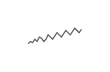
\begin{tikzpicture}[x=0.08em, y=0.08em, line width=0.4pt]
                \draw[FooterGray] (0,3) -- (1,4) -- (2,3.5) -- (3,5) -- (4,4) -- (5,6) -- (6,5.5) -- (7,4) -- (8,5) -- (9,7) -- (10,6) -- (11,5) -- (12,6.5) -- (13,8) -- (14,7) -- (15,6) -- (16,7.5) -- (17,9) -- (18,8) -- (19,7) -- (20,8.5) -- (21,10) -- (22,9) -- (23,8) -- (24,9.5);
            \end{tikzpicture}%
        }%
        \hskip0.5cm%
    }%
    \vskip6pt%
}

%=============================================================================
% PACKAGES
%=============================================================================
\usepackage[utf8]{inputenc}
\DeclareUnicodeCharacter{03B1}{\ensuremath{\alpha}}
\usepackage[T1]{fontenc}
\usepackage{amsmath, amssymb, amsthm}
\usepackage{mathtools}
\usepackage{bm}
\usepackage{tikz}
\usetikzlibrary{arrows.meta, positioning, shapes, calc, decorations.pathreplacing, shadings}
\usepackage{booktabs}
\usepackage{multirow}
\usepackage{array}
\usepackage{graphicx}
\usepackage{animate}
\usepackage{hyperref}
\usepackage{colortbl}
\usepackage{listings}
\lstset{language=Python, basicstyle=\ttfamily\scriptsize, keywordstyle=\color{MainBlue}\bfseries,
  commentstyle=\color{Forest}, stringstyle=\color{Crimson}, breaklines=true,
  frame=none, backgroundcolor=\color{VeryLightGray}, xleftmargin=2mm}
\hypersetup{colorlinks=true, linkcolor=MainBlue, urlcolor=MainBlue}
\graphicspath{{../../logos/}{../../charts/}{../../photos/}}
\usepackage{xcolor}
\hfuzz=2pt  % Suppress tiny overfull warnings (<2pt)
\vfuzz=2pt  % Suppress tiny vertical overfull warnings (<2pt)
% \mathrm in the sans-serif family of the slides (beamer resets \mathrm to the serif family at \begin{document};
% this hook runs after beamer's, so WN, Var, RMSE, ... in formulas match the surrounding text)
% Bold vectors and matrices in the same sans-serif family: \mathbf{A} in sans bold (beamer's own \mathbf came out in
% medium weight), and the bold upright Greek capitals of \boldsymbol / \bm (\bSigma, \bPhi, \boldsymbol{\Theta}) in
% cmss bold: bm.sty fixes its "boldoperators" font when it is loaded (serif cmbx), before beamer switches the
% operators to cmss, so it is reset here.
\AtBeginDocument{%
  \SetMathAlphabet{\mathrm}{normal}{\encodingdefault}{\sfdefault}{\mddefault}{n}%
  \SetMathAlphabet{\mathrm}{bold}{\encodingdefault}{\sfdefault}{bx}{n}%
  \SetMathAlphabet{\mathbf}{normal}{\encodingdefault}{\sfdefault}{bx}{n}%
  \SetMathAlphabet{\mathbf}{bold}{\encodingdefault}{\sfdefault}{bx}{n}%
  \SetSymbolFont{boldoperators}{normal}{OT1}{cmss}{bx}{n}%
  \SetSymbolFont{boldoperators}{bold}{OT1}{cmss}{bx}{n}}

%=============================================================================
% QUANTLET COMMANDS
%   \quantlet{<displayed name>}{<url>}       (generic, compatible with the older TSA decks)
%   \tsaquantlet{Ch_05}{TSA_ch5_garch}       -> https://github.com/danpele/Time-Series-Analysis/tree/main/Quantlets/Ch_05/TSA_ch5_garch
%   \qlurl{<folder>} is defined per chapter by the generator (Quantlets/Ch_NN/<folder>)
%=============================================================================
\newcommand{\tsarepo}{https://github.com/danpele/Time-Series-Analysis}
\newcommand{\tsaqlbase}{https://github.com/danpele/Time-Series-Analysis/tree/main/Quantlets}
\newcommand{\quantlet}[2]{%
    \hfill\href{#2}{%
        \raisebox{-0.15em}{
\includegraphics[height=0.7em]{ql_logo.png}}%
        \textcolor{MainBlue}{\tiny\ #1}%
    }%
}
\newcommand{\tsaquantlet}[2]{\quantlet{\detokenize{#2}}{\tsaqlbase/#1/#2}}

%=============================================================================
% NOTEBOOKS (Google Colab)
%   \colaburl{notebooks/EN/chapter5_seminar_notebook.ipynb} -> the Colab link of a file in the TSA repo
%   \nb: the chapter notebook (each seminar deck redefines it with \renewcommand)
%=============================================================================
\newcommand{\colaburl}[1]{https://colab.research.google.com/github/danpele/Time-Series-Analysis/blob/main/#1}
\newcommand{\nb}{https://colab.research.google.com/github/danpele/Time-Series-Analysis/tree/main/notebooks/EN}
\newcommand{\nbname}{notebooks/EN}

%=============================================================================
% SLIDE HELPERS (used by the generators; the same as in MFM)
%=============================================================================
% local font size for list bodies (the preamble forces \normalsize)
\newcommand{\itemsize}[1]{\setbeamertemplate{itemize/enumerate body begin}{#1}\setbeamertemplate{itemize/enumerate subbody begin}{#1}}
\newcommand{\intitle}[1]{{\hypersetup{urlcolor=white}#1}}   % white links inside coloured title bars
\newcommand{\imgcap}[1]{{\scriptsize #1}\\[0.5mm]}          % caption under a photo
\newcommand{\imgcredit}[2]{{\tiny\color{FooterGray}\href{#1}{#2}}}   % image credit: source URL, author/licence
\newcommand{\aiprompt}[1]{{\ttfamily\color{MainBlue}#1}}     % a prompt to an AI assistant

%=============================================================================
% SEMINARS: student version by default; the instructor wrapper *_solutions.tex sets \solutionstrue
%=============================================================================
\makeatletter\@ifundefined{ifsolutions}{\expandafter\newif\csname ifsolutions\endcsname}{}\makeatother
\newcommand{\solonly}[1]{\ifsolutions #1\fi}
\newcommand{\propsub}{\ifsolutions\else\framesubtitle{\ifdefined\tsalang Rezolvarea se discută la seminar\else Solution discussed in class\fi}\fi}

%=============================================================================
% APPENDIX AND CHAPTER LINKS (latex/appendix_links.py writes the calls; it also re-declares these
% macros before \begin{document}, so the decks compile with or without this preamble block)
%=============================================================================
\providecommand{\tsaapplink}[3]{\hypertarget{#2}{}\hyperlink{#1}{\beamergotobutton{#3}}}
\providecommand{\tsaappback}[2]{\begin{tikzpicture}[remember picture,overlay]\node[anchor=south east] at ([xshift=-3mm,yshift=7mm]current page.south east){\hyperlink{#1}{\beamerreturnbutton{#2}}};\end{tikzpicture}}
\providecommand{\tsachlink}[2]{\href{#1}{#2}}
\providecommand{\tsachlinkt}[2]{\href{#1}{\usebeamercolor[fg]{frametitle}#2}}

%=============================================================================
% QUANTINAR COMMAND: link către un curs Quantinar (subiecte avansate)
%=============================================================================
\newcommand{\quantinar}[2]{%
    \href{#2}{%
        \raisebox{-0.15em}{
\includegraphics[height=0.8em]{qr_logo.png}}%
        \textcolor{MainBlue}{\scriptsize\ #1}%
    }%
}

%=============================================================================
% CUSTOM TITLE PAGE
%=============================================================================
\defbeamertemplate*{title page}{hybrid}[1][]
{
    \vspace{0.2cm}
    % Logos row - top header (with clickable links)
    \begin{center}
        \href{https://www.ase.ro}{
\includegraphics[height=1.0cm]{ase_logo.png}}\hspace{0.3cm}%
        \href{https://theida.net}{
\includegraphics[height=1.0cm]{ida_logo.png}}\hspace{0.3cm}%
        \href{https://blockchain-research-center.com}{
\includegraphics[height=1.0cm]{brc_logo.png}}\hspace{0.3cm}%
        \href{https://www.ai4efin.ase.ro}{
\includegraphics[height=1.0cm]{ai4efin_logo.png}}\hspace{0.3cm}%
        \href{https://ipe.ro/new}{
\includegraphics[height=1.0cm]{acad_logo.png}}\hspace{0.3cm}%
        \href{https://www.digital-finance-msca.com}{
\includegraphics[height=1.0cm]{msca_logo.png}}%
    \end{center}

    \vspace{0.6cm}

    % Main title with Q logos on sides (with clickable links)
    \begin{center}
        \begin{minipage}{0.1\textwidth}
            \centering
            \href{https://quantlet.com}{
\includegraphics[height=1.1cm]{ql_logo.png}}
        \end{minipage}%
        \begin{minipage}{0.78\textwidth}
            \centering
            {\LARGE\bfseries\usebeamercolor[fg]{title}\inserttitle}

            \vspace{0.3cm}

            {\usebeamerfont{subtitle}\usebeamercolor[fg]{title}\insertsubtitle}
        \end{minipage}%
        \begin{minipage}{0.1\textwidth}
            \centering
            \href{https://quantinar.com}{
\includegraphics[height=1.1cm]{qr_logo.png}}
        \end{minipage}
    \end{center}

    \vspace{0.6cm}

    % Authors (left aligned)
    \hspace{0.5cm}{\usebeamerfont{author}\insertauthor}

    \vspace{0.3cm}

    % Institute/Affiliations (left aligned)
    \hspace{0.5cm}\begin{minipage}[t]{0.9\textwidth}
        \raggedright\small\insertinstitute
    \end{minipage}
}

%=============================================================================
% THEOREM ENVIRONMENTS
%=============================================================================
\theoremstyle{definition}
\setbeamertemplate{theorems}[numbered]
\ifdefined\tsalang
\newtheorem{defn}{Definiție}
\newtheorem{thm}{Teoremă}
\newtheorem{prop}{Propoziție}
\newtheorem{rmk}{Observație}
\else
\newtheorem{defn}{Definition}
\newtheorem{thm}{Theorem}
\newtheorem{prop}{Proposition}
\newtheorem{rmk}{Remark}
\fi

%=============================================================================
% CENTRED MINIPAGE (no extra vertical space)
%=============================================================================
\newenvironment{cminipage}[1]{%
    \par\noindent\hfill\begin{minipage}{#1}\ignorespaces
}{%
    \end{minipage}\hfill\null\par
}

%=============================================================================
% CUSTOM COMMANDS
%=============================================================================
\newcommand{\E}{\mathbb{E}}
\newcommand{\Var}{\text{Var}}
\newcommand{\Cov}{\text{Cov}}
\newcommand{\Corr}{\text{Corr}}
\newcommand{\R}{\mathbb{R}}
\newcommand{\N}{\mathbb{N}}
\newcommand{\Z}{\mathbb{Z}}
\newcommand{\B}{\mathbf{B}}
\newcommand{\imark}{\textcolor{MainBlue}{\textbullet}}
\newcommand{\RMSE}{\text{RMSE}}
\newcommand{\MAE}{\text{MAE}}
\newcommand{\MAPE}{\text{MAPE}}

% Boldface vector/matrix commands (VAR, VECM, state space; also used by the older TSA decks)
\newcommand{\bY}{\mathbf{Y}}
\newcommand{\bX}{\mathbf{X}}
\newcommand{\bA}{\mathbf{A}}
\newcommand{\bB}{\mathbf{B}}
\newcommand{\bepsilon}{\boldsymbol{\varepsilon}}
\newcommand{\bSigma}{\boldsymbol{\Sigma}}
\newcommand{\bPhi}{\boldsymbol{\Phi}}
\newcommand{\bGamma}{\boldsymbol{\Gamma}}
\newcommand{\bPi}{\boldsymbol{\Pi}}
\newcommand{\bc}{\mathbf{c}}
\newcommand{\balpha}{\boldsymbol{\alpha}}
\newcommand{\bbeta}{\boldsymbol{\beta}}
\newcommand{\bvarepsilon}{\boldsymbol{\varepsilon}}

% Legacy seminar marks (older TSA seminar decks)
\newcommand{\correct}{\textcolor{Forest}{\checkmark}}
\newcommand{\incorrect}{\textcolor{Crimson}{\texttimes}}
 se definește
%   \newcommand{\coursename}{Time Series Analysis}      (EN)
%   \newcommand{\coursename}{Serii de timp}       (RO)  și  \def\tsalang{ro}
% Fișierele .tex se află în EN/Courses, EN/Seminars, RO/Cursuri, RO/Seminarii (două niveluri sub rădăcină).
% Deck-urile sînt generate de latex/build_chapterN.py / build_seminarN.py (vezi latex/tsa_build.py).

\documentclass[9pt, aspectratio=169, t]{beamer}
\providecommand{\coursename}{Time Series Analysis}

% Ensure content fits on slides
\setbeamersize{text margin left=8mm, text margin right=8mm}
% Smaller institute font (title page)
\setbeamerfont{institute}{size=\footnotesize}

%=============================================================================
% THEME AND STYLE CONFIGURATION
%=============================================================================
\usetheme{default}
% Using default theme for clean header/footer control

% Color Palette (matching Redispatch PDF)
\definecolor{MainBlue}{RGB}{26, 58, 110}
\definecolor{AccentBlue}{RGB}{26, 58, 110}
\definecolor{IDAred}{RGB}{205, 0, 0}
\definecolor{DarkGray}{RGB}{51, 51, 51}
\definecolor{MediumGray}{RGB}{128, 128, 128}
\definecolor{LightGray}{RGB}{248, 248, 248}
\definecolor{VeryLightGray}{RGB}{235, 235, 235}
\definecolor{KeynoteGray}{RGB}{218, 218, 218}
\definecolor{SectionGray}{RGB}{120, 120, 120}
\definecolor{FooterGray}{RGB}{100, 100, 100}
\definecolor{Crimson}{RGB}{220, 53, 69}
\definecolor{Forest}{RGB}{46, 125, 50}
\definecolor{Amber}{RGB}{181, 133, 63}
\definecolor{Orange}{RGB}{230, 126, 34}
\definecolor{Purple}{RGB}{142, 68, 173}

% Gradient background (exact Keynote 315° gradient: white to RGB 218,218,218)
\setbeamertemplate{background}{%
    \begin{tikzpicture}[remember picture, overlay]
        \shade[shading=axis, shading angle=315,
        top color=white, bottom color=KeynoteGray]
        (current page.south west) rectangle (current page.north east);
    \end{tikzpicture}%
}
% Fallback solid color for compatibility
\setbeamercolor{background canvas}{bg=}

\setbeamercolor{palette primary}{bg=MainBlue, fg=white}
\setbeamercolor{palette secondary}{bg=MainBlue!85, fg=white}
\setbeamercolor{palette tertiary}{bg=MainBlue!70, fg=white}
\setbeamercolor{structure}{fg=MainBlue}
\setbeamercolor{title}{fg=IDAred}
\setbeamercolor{frametitle}{fg=IDAred, bg=}
\setbeamercolor{block title}{bg=MainBlue, fg=white}
\setbeamercolor{block body}{bg=VeryLightGray, fg=DarkGray}
\setbeamercolor{block title alerted}{bg=Crimson, fg=white}
\setbeamercolor{block body alerted}{bg=Crimson!8, fg=DarkGray}
\setbeamercolor{block title example}{bg=Forest, fg=white}
\setbeamercolor{block body example}{bg=Forest!8, fg=DarkGray}
\setbeamercolor{item}{fg=MainBlue}

% Footer colors (override Madrid theme blue)
\setbeamercolor{author in head/foot}{fg=FooterGray, bg=}
\setbeamercolor{title in head/foot}{fg=FooterGray, bg=}
\setbeamercolor{date in head/foot}{fg=FooterGray, bg=}
\setbeamercolor{section in head/foot}{fg=FooterGray, bg=}
\setbeamercolor{subsection in head/foot}{fg=FooterGray, bg=}

% Bullet styles (apply everywhere including blocks)
\setbeamertemplate{itemize item}{\color{MainBlue}$\boxdot$}
\setbeamertemplate{itemize subitem}{\color{MainBlue}$\blacktriangleright$}
\setbeamertemplate{itemize subsubitem}{\color{MainBlue}\tiny$\bullet$}
\setbeamertemplate{itemize/enumerate body begin}{\normalsize}
\setbeamertemplate{itemize/enumerate subbody begin}{\normalsize}

% Item spacing - compact style
\setlength{\leftmargini}{10pt}       % Level 1: minimal indent
\setlength{\leftmarginii}{10pt}      % Level 2: minimal additional indent
% Compact list spacing (zero extra space before/after lists in blocks)
\makeatletter
\def\@listi{\leftmargin\leftmargini \topsep 0pt \parsep 0pt \itemsep 0pt}
\def\@listii{\leftmargin\leftmarginii \topsep 0pt \parsep 0pt \itemsep 0pt}
\makeatother

\setbeamertemplate{navigation symbols}{}

%=============================================================================
% CUSTOM HEADLINE
%=============================================================================
\setbeamertemplate{headline}{%
    \vskip10pt%
    \hbox to \paperwidth{%
        \hskip0.5cm%
        {\small\color{FooterGray}\renewcommand{\hyperlink}[2]{##2}\insertsectionhead}%
        \hfill%
        \textcolor{FooterGray}{\small\insertframenumber}%
        \hskip0.5cm%
    }%
    \vskip4pt%
    {\color{FooterGray}\hrule height 0.4pt}%
}

%=============================================================================
% CUSTOM FOOTER
%=============================================================================
\usepackage{fontawesome5}

\setbeamertemplate{footline}{%
    {\color{FooterGray}\hrule height 0.4pt}%
    \vskip4pt%
    \hbox to \paperwidth{%
        \hskip0.5cm%
        \textcolor{FooterGray}{\small\coursename}%
        \hfill%
        \raisebox{-0.1em}{%
            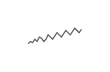
\begin{tikzpicture}[x=0.08em, y=0.08em, line width=0.4pt]
                \draw[FooterGray] (0,3) -- (1,4) -- (2,3.5) -- (3,5) -- (4,4) -- (5,6) -- (6,5.5) -- (7,4) -- (8,5) -- (9,7) -- (10,6) -- (11,5) -- (12,6.5) -- (13,8) -- (14,7) -- (15,6) -- (16,7.5) -- (17,9) -- (18,8) -- (19,7) -- (20,8.5) -- (21,10) -- (22,9) -- (23,8) -- (24,9.5);
            \end{tikzpicture}%
        }%
        \hskip0.5cm%
    }%
    \vskip6pt%
}

%=============================================================================
% PACKAGES
%=============================================================================
\usepackage[utf8]{inputenc}
\DeclareUnicodeCharacter{03B1}{\ensuremath{\alpha}}
\usepackage[T1]{fontenc}
\usepackage{amsmath, amssymb, amsthm}
\usepackage{mathtools}
\usepackage{bm}
\usepackage{tikz}
\usetikzlibrary{arrows.meta, positioning, shapes, calc, decorations.pathreplacing, shadings}
\usepackage{booktabs}
\usepackage{multirow}
\usepackage{array}
\usepackage{graphicx}
\usepackage{animate}
\usepackage{hyperref}
\usepackage{colortbl}
\usepackage{listings}
\lstset{language=Python, basicstyle=\ttfamily\scriptsize, keywordstyle=\color{MainBlue}\bfseries,
  commentstyle=\color{Forest}, stringstyle=\color{Crimson}, breaklines=true,
  frame=none, backgroundcolor=\color{VeryLightGray}, xleftmargin=2mm}
\hypersetup{colorlinks=true, linkcolor=MainBlue, urlcolor=MainBlue}
\graphicspath{{../../logos/}{../../charts/}{../../photos/}}
\usepackage{xcolor}
\hfuzz=2pt  % Suppress tiny overfull warnings (<2pt)
\vfuzz=2pt  % Suppress tiny vertical overfull warnings (<2pt)
% \mathrm in the sans-serif family of the slides (beamer resets \mathrm to the serif family at \begin{document};
% this hook runs after beamer's, so WN, Var, RMSE, ... in formulas match the surrounding text)
% Bold vectors and matrices in the same sans-serif family: \mathbf{A} in sans bold (beamer's own \mathbf came out in
% medium weight), and the bold upright Greek capitals of \boldsymbol / \bm (\bSigma, \bPhi, \boldsymbol{\Theta}) in
% cmss bold: bm.sty fixes its "boldoperators" font when it is loaded (serif cmbx), before beamer switches the
% operators to cmss, so it is reset here.
\AtBeginDocument{%
  \SetMathAlphabet{\mathrm}{normal}{\encodingdefault}{\sfdefault}{\mddefault}{n}%
  \SetMathAlphabet{\mathrm}{bold}{\encodingdefault}{\sfdefault}{bx}{n}%
  \SetMathAlphabet{\mathbf}{normal}{\encodingdefault}{\sfdefault}{bx}{n}%
  \SetMathAlphabet{\mathbf}{bold}{\encodingdefault}{\sfdefault}{bx}{n}%
  \SetSymbolFont{boldoperators}{normal}{OT1}{cmss}{bx}{n}%
  \SetSymbolFont{boldoperators}{bold}{OT1}{cmss}{bx}{n}}

%=============================================================================
% QUANTLET COMMANDS
%   \quantlet{<displayed name>}{<url>}       (generic, compatible with the older TSA decks)
%   \tsaquantlet{Ch_05}{TSA_ch5_garch}       -> https://github.com/danpele/Time-Series-Analysis/tree/main/Quantlets/Ch_05/TSA_ch5_garch
%   \qlurl{<folder>} is defined per chapter by the generator (Quantlets/Ch_NN/<folder>)
%=============================================================================
\newcommand{\tsarepo}{https://github.com/danpele/Time-Series-Analysis}
\newcommand{\tsaqlbase}{https://github.com/danpele/Time-Series-Analysis/tree/main/Quantlets}
\newcommand{\quantlet}[2]{%
    \hfill\href{#2}{%
        \raisebox{-0.15em}{
\includegraphics[height=0.7em]{ql_logo.png}}%
        \textcolor{MainBlue}{\tiny\ #1}%
    }%
}
\newcommand{\tsaquantlet}[2]{\quantlet{\detokenize{#2}}{\tsaqlbase/#1/#2}}

%=============================================================================
% NOTEBOOKS (Google Colab)
%   \colaburl{notebooks/EN/chapter5_seminar_notebook.ipynb} -> the Colab link of a file in the TSA repo
%   \nb: the chapter notebook (each seminar deck redefines it with \renewcommand)
%=============================================================================
\newcommand{\colaburl}[1]{https://colab.research.google.com/github/danpele/Time-Series-Analysis/blob/main/#1}
\newcommand{\nb}{https://colab.research.google.com/github/danpele/Time-Series-Analysis/tree/main/notebooks/EN}
\newcommand{\nbname}{notebooks/EN}

%=============================================================================
% SLIDE HELPERS (used by the generators; the same as in MFM)
%=============================================================================
% local font size for list bodies (the preamble forces \normalsize)
\newcommand{\itemsize}[1]{\setbeamertemplate{itemize/enumerate body begin}{#1}\setbeamertemplate{itemize/enumerate subbody begin}{#1}}
\newcommand{\intitle}[1]{{\hypersetup{urlcolor=white}#1}}   % white links inside coloured title bars
\newcommand{\imgcap}[1]{{\scriptsize #1}\\[0.5mm]}          % caption under a photo
\newcommand{\imgcredit}[2]{{\tiny\color{FooterGray}\href{#1}{#2}}}   % image credit: source URL, author/licence
\newcommand{\aiprompt}[1]{{\ttfamily\color{MainBlue}#1}}     % a prompt to an AI assistant

%=============================================================================
% SEMINARS: student version by default; the instructor wrapper *_solutions.tex sets \solutionstrue
%=============================================================================
\makeatletter\@ifundefined{ifsolutions}{\expandafter\newif\csname ifsolutions\endcsname}{}\makeatother
\newcommand{\solonly}[1]{\ifsolutions #1\fi}
\newcommand{\propsub}{\ifsolutions\else\framesubtitle{\ifdefined\tsalang Rezolvarea se discută la seminar\else Solution discussed in class\fi}\fi}

%=============================================================================
% APPENDIX AND CHAPTER LINKS (latex/appendix_links.py writes the calls; it also re-declares these
% macros before \begin{document}, so the decks compile with or without this preamble block)
%=============================================================================
\providecommand{\tsaapplink}[3]{\hypertarget{#2}{}\hyperlink{#1}{\beamergotobutton{#3}}}
\providecommand{\tsaappback}[2]{\begin{tikzpicture}[remember picture,overlay]\node[anchor=south east] at ([xshift=-3mm,yshift=7mm]current page.south east){\hyperlink{#1}{\beamerreturnbutton{#2}}};\end{tikzpicture}}
\providecommand{\tsachlink}[2]{\href{#1}{#2}}
\providecommand{\tsachlinkt}[2]{\href{#1}{\usebeamercolor[fg]{frametitle}#2}}

%=============================================================================
% QUANTINAR COMMAND: link către un curs Quantinar (subiecte avansate)
%=============================================================================
\newcommand{\quantinar}[2]{%
    \href{#2}{%
        \raisebox{-0.15em}{
\includegraphics[height=0.8em]{qr_logo.png}}%
        \textcolor{MainBlue}{\scriptsize\ #1}%
    }%
}

%=============================================================================
% CUSTOM TITLE PAGE
%=============================================================================
\defbeamertemplate*{title page}{hybrid}[1][]
{
    \vspace{0.2cm}
    % Logos row - top header (with clickable links)
    \begin{center}
        \href{https://www.ase.ro}{
\includegraphics[height=1.0cm]{ase_logo.png}}\hspace{0.3cm}%
        \href{https://theida.net}{
\includegraphics[height=1.0cm]{ida_logo.png}}\hspace{0.3cm}%
        \href{https://blockchain-research-center.com}{
\includegraphics[height=1.0cm]{brc_logo.png}}\hspace{0.3cm}%
        \href{https://www.ai4efin.ase.ro}{
\includegraphics[height=1.0cm]{ai4efin_logo.png}}\hspace{0.3cm}%
        \href{https://ipe.ro/new}{
\includegraphics[height=1.0cm]{acad_logo.png}}\hspace{0.3cm}%
        \href{https://www.digital-finance-msca.com}{
\includegraphics[height=1.0cm]{msca_logo.png}}%
    \end{center}

    \vspace{0.6cm}

    % Main title with Q logos on sides (with clickable links)
    \begin{center}
        \begin{minipage}{0.1\textwidth}
            \centering
            \href{https://quantlet.com}{
\includegraphics[height=1.1cm]{ql_logo.png}}
        \end{minipage}%
        \begin{minipage}{0.78\textwidth}
            \centering
            {\LARGE\bfseries\usebeamercolor[fg]{title}\inserttitle}

            \vspace{0.3cm}

            {\usebeamerfont{subtitle}\usebeamercolor[fg]{title}\insertsubtitle}
        \end{minipage}%
        \begin{minipage}{0.1\textwidth}
            \centering
            \href{https://quantinar.com}{
\includegraphics[height=1.1cm]{qr_logo.png}}
        \end{minipage}
    \end{center}

    \vspace{0.6cm}

    % Authors (left aligned)
    \hspace{0.5cm}{\usebeamerfont{author}\insertauthor}

    \vspace{0.3cm}

    % Institute/Affiliations (left aligned)
    \hspace{0.5cm}\begin{minipage}[t]{0.9\textwidth}
        \raggedright\small\insertinstitute
    \end{minipage}
}

%=============================================================================
% THEOREM ENVIRONMENTS
%=============================================================================
\theoremstyle{definition}
\setbeamertemplate{theorems}[numbered]
\ifdefined\tsalang
\newtheorem{defn}{Definiție}
\newtheorem{thm}{Teoremă}
\newtheorem{prop}{Propoziție}
\newtheorem{rmk}{Observație}
\else
\newtheorem{defn}{Definition}
\newtheorem{thm}{Theorem}
\newtheorem{prop}{Proposition}
\newtheorem{rmk}{Remark}
\fi

%=============================================================================
% CENTRED MINIPAGE (no extra vertical space)
%=============================================================================
\newenvironment{cminipage}[1]{%
    \par\noindent\hfill\begin{minipage}{#1}\ignorespaces
}{%
    \end{minipage}\hfill\null\par
}

%=============================================================================
% CUSTOM COMMANDS
%=============================================================================
\newcommand{\E}{\mathbb{E}}
\newcommand{\Var}{\text{Var}}
\newcommand{\Cov}{\text{Cov}}
\newcommand{\Corr}{\text{Corr}}
\newcommand{\R}{\mathbb{R}}
\newcommand{\N}{\mathbb{N}}
\newcommand{\Z}{\mathbb{Z}}
\newcommand{\B}{\mathbf{B}}
\newcommand{\imark}{\textcolor{MainBlue}{\textbullet}}
\newcommand{\RMSE}{\text{RMSE}}
\newcommand{\MAE}{\text{MAE}}
\newcommand{\MAPE}{\text{MAPE}}

% Boldface vector/matrix commands (VAR, VECM, state space; also used by the older TSA decks)
\newcommand{\bY}{\mathbf{Y}}
\newcommand{\bX}{\mathbf{X}}
\newcommand{\bA}{\mathbf{A}}
\newcommand{\bB}{\mathbf{B}}
\newcommand{\bepsilon}{\boldsymbol{\varepsilon}}
\newcommand{\bSigma}{\boldsymbol{\Sigma}}
\newcommand{\bPhi}{\boldsymbol{\Phi}}
\newcommand{\bGamma}{\boldsymbol{\Gamma}}
\newcommand{\bPi}{\boldsymbol{\Pi}}
\newcommand{\bc}{\mathbf{c}}
\newcommand{\balpha}{\boldsymbol{\alpha}}
\newcommand{\bbeta}{\boldsymbol{\beta}}
\newcommand{\bvarepsilon}{\boldsymbol{\varepsilon}}

% Legacy seminar marks (older TSA seminar decks)
\newcommand{\correct}{\textcolor{Forest}{\checkmark}}
\newcommand{\incorrect}{\textcolor{Crimson}{\texttimes}}
 se definește
%   \newcommand{\coursename}{Time Series Analysis}      (EN)
%   \newcommand{\coursename}{Serii de timp}       (RO)  și  \def\tsalang{ro}
% Fișierele .tex se află în EN/Courses, EN/Seminars, RO/Cursuri, RO/Seminarii (două niveluri sub rădăcină).
% Deck-urile sînt generate de latex/build_chapterN.py / build_seminarN.py (vezi latex/tsa_build.py).

\documentclass[9pt, aspectratio=169, t]{beamer}
\providecommand{\coursename}{Time Series Analysis}

% Ensure content fits on slides
\setbeamersize{text margin left=8mm, text margin right=8mm}
% Smaller institute font (title page)
\setbeamerfont{institute}{size=\footnotesize}

%=============================================================================
% THEME AND STYLE CONFIGURATION
%=============================================================================
\usetheme{default}
% Using default theme for clean header/footer control

% Color Palette (matching Redispatch PDF)
\definecolor{MainBlue}{RGB}{26, 58, 110}
\definecolor{AccentBlue}{RGB}{26, 58, 110}
\definecolor{IDAred}{RGB}{205, 0, 0}
\definecolor{DarkGray}{RGB}{51, 51, 51}
\definecolor{MediumGray}{RGB}{128, 128, 128}
\definecolor{LightGray}{RGB}{248, 248, 248}
\definecolor{VeryLightGray}{RGB}{235, 235, 235}
\definecolor{KeynoteGray}{RGB}{218, 218, 218}
\definecolor{SectionGray}{RGB}{120, 120, 120}
\definecolor{FooterGray}{RGB}{100, 100, 100}
\definecolor{Crimson}{RGB}{220, 53, 69}
\definecolor{Forest}{RGB}{46, 125, 50}
\definecolor{Amber}{RGB}{181, 133, 63}
\definecolor{Orange}{RGB}{230, 126, 34}
\definecolor{Purple}{RGB}{142, 68, 173}

% Gradient background (exact Keynote 315° gradient: white to RGB 218,218,218)
\setbeamertemplate{background}{%
    \begin{tikzpicture}[remember picture, overlay]
        \shade[shading=axis, shading angle=315,
        top color=white, bottom color=KeynoteGray]
        (current page.south west) rectangle (current page.north east);
    \end{tikzpicture}%
}
% Fallback solid color for compatibility
\setbeamercolor{background canvas}{bg=}

\setbeamercolor{palette primary}{bg=MainBlue, fg=white}
\setbeamercolor{palette secondary}{bg=MainBlue!85, fg=white}
\setbeamercolor{palette tertiary}{bg=MainBlue!70, fg=white}
\setbeamercolor{structure}{fg=MainBlue}
\setbeamercolor{title}{fg=IDAred}
\setbeamercolor{frametitle}{fg=IDAred, bg=}
\setbeamercolor{block title}{bg=MainBlue, fg=white}
\setbeamercolor{block body}{bg=VeryLightGray, fg=DarkGray}
\setbeamercolor{block title alerted}{bg=Crimson, fg=white}
\setbeamercolor{block body alerted}{bg=Crimson!8, fg=DarkGray}
\setbeamercolor{block title example}{bg=Forest, fg=white}
\setbeamercolor{block body example}{bg=Forest!8, fg=DarkGray}
\setbeamercolor{item}{fg=MainBlue}

% Footer colors (override Madrid theme blue)
\setbeamercolor{author in head/foot}{fg=FooterGray, bg=}
\setbeamercolor{title in head/foot}{fg=FooterGray, bg=}
\setbeamercolor{date in head/foot}{fg=FooterGray, bg=}
\setbeamercolor{section in head/foot}{fg=FooterGray, bg=}
\setbeamercolor{subsection in head/foot}{fg=FooterGray, bg=}

% Bullet styles (apply everywhere including blocks)
\setbeamertemplate{itemize item}{\color{MainBlue}$\boxdot$}
\setbeamertemplate{itemize subitem}{\color{MainBlue}$\blacktriangleright$}
\setbeamertemplate{itemize subsubitem}{\color{MainBlue}\tiny$\bullet$}
\setbeamertemplate{itemize/enumerate body begin}{\normalsize}
\setbeamertemplate{itemize/enumerate subbody begin}{\normalsize}

% Item spacing - compact style
\setlength{\leftmargini}{10pt}       % Level 1: minimal indent
\setlength{\leftmarginii}{10pt}      % Level 2: minimal additional indent
% Compact list spacing (zero extra space before/after lists in blocks)
\makeatletter
\def\@listi{\leftmargin\leftmargini \topsep 0pt \parsep 0pt \itemsep 0pt}
\def\@listii{\leftmargin\leftmarginii \topsep 0pt \parsep 0pt \itemsep 0pt}
\makeatother

\setbeamertemplate{navigation symbols}{}

%=============================================================================
% CUSTOM HEADLINE
%=============================================================================
\setbeamertemplate{headline}{%
    \vskip10pt%
    \hbox to \paperwidth{%
        \hskip0.5cm%
        {\small\color{FooterGray}\renewcommand{\hyperlink}[2]{##2}\insertsectionhead}%
        \hfill%
        \textcolor{FooterGray}{\small\insertframenumber}%
        \hskip0.5cm%
    }%
    \vskip4pt%
    {\color{FooterGray}\hrule height 0.4pt}%
}

%=============================================================================
% CUSTOM FOOTER
%=============================================================================
\usepackage{fontawesome5}

\setbeamertemplate{footline}{%
    {\color{FooterGray}\hrule height 0.4pt}%
    \vskip4pt%
    \hbox to \paperwidth{%
        \hskip0.5cm%
        \textcolor{FooterGray}{\small\coursename}%
        \hfill%
        \raisebox{-0.1em}{%
            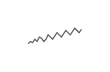
\begin{tikzpicture}[x=0.08em, y=0.08em, line width=0.4pt]
                \draw[FooterGray] (0,3) -- (1,4) -- (2,3.5) -- (3,5) -- (4,4) -- (5,6) -- (6,5.5) -- (7,4) -- (8,5) -- (9,7) -- (10,6) -- (11,5) -- (12,6.5) -- (13,8) -- (14,7) -- (15,6) -- (16,7.5) -- (17,9) -- (18,8) -- (19,7) -- (20,8.5) -- (21,10) -- (22,9) -- (23,8) -- (24,9.5);
            \end{tikzpicture}%
        }%
        \hskip0.5cm%
    }%
    \vskip6pt%
}

%=============================================================================
% PACKAGES
%=============================================================================
\usepackage[utf8]{inputenc}
\DeclareUnicodeCharacter{03B1}{\ensuremath{\alpha}}
\usepackage[T1]{fontenc}
\usepackage{amsmath, amssymb, amsthm}
\usepackage{mathtools}
\usepackage{bm}
\usepackage{tikz}
\usetikzlibrary{arrows.meta, positioning, shapes, calc, decorations.pathreplacing, shadings}
\usepackage{booktabs}
\usepackage{multirow}
\usepackage{array}
\usepackage{graphicx}
\usepackage{animate}
\usepackage{hyperref}
\usepackage{colortbl}
\usepackage{listings}
\lstset{language=Python, basicstyle=\ttfamily\scriptsize, keywordstyle=\color{MainBlue}\bfseries,
  commentstyle=\color{Forest}, stringstyle=\color{Crimson}, breaklines=true,
  frame=none, backgroundcolor=\color{VeryLightGray}, xleftmargin=2mm}
\hypersetup{colorlinks=true, linkcolor=MainBlue, urlcolor=MainBlue}
\graphicspath{{../../logos/}{../../charts/}{../../photos/}}
\usepackage{xcolor}
\hfuzz=2pt  % Suppress tiny overfull warnings (<2pt)
\vfuzz=2pt  % Suppress tiny vertical overfull warnings (<2pt)
% \mathrm in the sans-serif family of the slides (beamer resets \mathrm to the serif family at \begin{document};
% this hook runs after beamer's, so WN, Var, RMSE, ... in formulas match the surrounding text)
% Bold vectors and matrices in the same sans-serif family: \mathbf{A} in sans bold (beamer's own \mathbf came out in
% medium weight), and the bold upright Greek capitals of \boldsymbol / \bm (\bSigma, \bPhi, \boldsymbol{\Theta}) in
% cmss bold: bm.sty fixes its "boldoperators" font when it is loaded (serif cmbx), before beamer switches the
% operators to cmss, so it is reset here.
\AtBeginDocument{%
  \SetMathAlphabet{\mathrm}{normal}{\encodingdefault}{\sfdefault}{\mddefault}{n}%
  \SetMathAlphabet{\mathrm}{bold}{\encodingdefault}{\sfdefault}{bx}{n}%
  \SetMathAlphabet{\mathbf}{normal}{\encodingdefault}{\sfdefault}{bx}{n}%
  \SetMathAlphabet{\mathbf}{bold}{\encodingdefault}{\sfdefault}{bx}{n}%
  \SetSymbolFont{boldoperators}{normal}{OT1}{cmss}{bx}{n}%
  \SetSymbolFont{boldoperators}{bold}{OT1}{cmss}{bx}{n}}

%=============================================================================
% QUANTLET COMMANDS
%   \quantlet{<displayed name>}{<url>}       (generic, compatible with the older TSA decks)
%   \tsaquantlet{Ch_05}{TSA_ch5_garch}       -> https://github.com/danpele/Time-Series-Analysis/tree/main/Quantlets/Ch_05/TSA_ch5_garch
%   \qlurl{<folder>} is defined per chapter by the generator (Quantlets/Ch_NN/<folder>)
%=============================================================================
\newcommand{\tsarepo}{https://github.com/danpele/Time-Series-Analysis}
\newcommand{\tsaqlbase}{https://github.com/danpele/Time-Series-Analysis/tree/main/Quantlets}
\newcommand{\quantlet}[2]{%
    \hfill\href{#2}{%
        \raisebox{-0.15em}{
\includegraphics[height=0.7em]{ql_logo.png}}%
        \textcolor{MainBlue}{\tiny\ #1}%
    }%
}
\newcommand{\tsaquantlet}[2]{\quantlet{\detokenize{#2}}{\tsaqlbase/#1/#2}}

%=============================================================================
% NOTEBOOKS (Google Colab)
%   \colaburl{notebooks/EN/chapter5_seminar_notebook.ipynb} -> the Colab link of a file in the TSA repo
%   \nb: the chapter notebook (each seminar deck redefines it with \renewcommand)
%=============================================================================
\newcommand{\colaburl}[1]{https://colab.research.google.com/github/danpele/Time-Series-Analysis/blob/main/#1}
\newcommand{\nb}{https://colab.research.google.com/github/danpele/Time-Series-Analysis/tree/main/notebooks/EN}
\newcommand{\nbname}{notebooks/EN}

%=============================================================================
% SLIDE HELPERS (used by the generators; the same as in MFM)
%=============================================================================
% local font size for list bodies (the preamble forces \normalsize)
\newcommand{\itemsize}[1]{\setbeamertemplate{itemize/enumerate body begin}{#1}\setbeamertemplate{itemize/enumerate subbody begin}{#1}}
\newcommand{\intitle}[1]{{\hypersetup{urlcolor=white}#1}}   % white links inside coloured title bars
\newcommand{\imgcap}[1]{{\scriptsize #1}\\[0.5mm]}          % caption under a photo
\newcommand{\imgcredit}[2]{{\tiny\color{FooterGray}\href{#1}{#2}}}   % image credit: source URL, author/licence
\newcommand{\aiprompt}[1]{{\ttfamily\color{MainBlue}#1}}     % a prompt to an AI assistant

%=============================================================================
% SEMINARS: student version by default; the instructor wrapper *_solutions.tex sets \solutionstrue
%=============================================================================
\makeatletter\@ifundefined{ifsolutions}{\expandafter\newif\csname ifsolutions\endcsname}{}\makeatother
\newcommand{\solonly}[1]{\ifsolutions #1\fi}
\newcommand{\propsub}{\ifsolutions\else\framesubtitle{\ifdefined\tsalang Rezolvarea se discută la seminar\else Solution discussed in class\fi}\fi}

%=============================================================================
% APPENDIX AND CHAPTER LINKS (latex/appendix_links.py writes the calls; it also re-declares these
% macros before \begin{document}, so the decks compile with or without this preamble block)
%=============================================================================
\providecommand{\tsaapplink}[3]{\hypertarget{#2}{}\hyperlink{#1}{\beamergotobutton{#3}}}
\providecommand{\tsaappback}[2]{\begin{tikzpicture}[remember picture,overlay]\node[anchor=south east] at ([xshift=-3mm,yshift=7mm]current page.south east){\hyperlink{#1}{\beamerreturnbutton{#2}}};\end{tikzpicture}}
\providecommand{\tsachlink}[2]{\href{#1}{#2}}
\providecommand{\tsachlinkt}[2]{\href{#1}{\usebeamercolor[fg]{frametitle}#2}}

%=============================================================================
% QUANTINAR COMMAND: link către un curs Quantinar (subiecte avansate)
%=============================================================================
\newcommand{\quantinar}[2]{%
    \href{#2}{%
        \raisebox{-0.15em}{
\includegraphics[height=0.8em]{qr_logo.png}}%
        \textcolor{MainBlue}{\scriptsize\ #1}%
    }%
}

%=============================================================================
% CUSTOM TITLE PAGE
%=============================================================================
\defbeamertemplate*{title page}{hybrid}[1][]
{
    \vspace{0.2cm}
    % Logos row - top header (with clickable links)
    \begin{center}
        \href{https://www.ase.ro}{
\includegraphics[height=1.0cm]{ase_logo.png}}\hspace{0.3cm}%
        \href{https://theida.net}{
\includegraphics[height=1.0cm]{ida_logo.png}}\hspace{0.3cm}%
        \href{https://blockchain-research-center.com}{
\includegraphics[height=1.0cm]{brc_logo.png}}\hspace{0.3cm}%
        \href{https://www.ai4efin.ase.ro}{
\includegraphics[height=1.0cm]{ai4efin_logo.png}}\hspace{0.3cm}%
        \href{https://ipe.ro/new}{
\includegraphics[height=1.0cm]{acad_logo.png}}\hspace{0.3cm}%
        \href{https://www.digital-finance-msca.com}{
\includegraphics[height=1.0cm]{msca_logo.png}}%
    \end{center}

    \vspace{0.6cm}

    % Main title with Q logos on sides (with clickable links)
    \begin{center}
        \begin{minipage}{0.1\textwidth}
            \centering
            \href{https://quantlet.com}{
\includegraphics[height=1.1cm]{ql_logo.png}}
        \end{minipage}%
        \begin{minipage}{0.78\textwidth}
            \centering
            {\LARGE\bfseries\usebeamercolor[fg]{title}\inserttitle}

            \vspace{0.3cm}

            {\usebeamerfont{subtitle}\usebeamercolor[fg]{title}\insertsubtitle}
        \end{minipage}%
        \begin{minipage}{0.1\textwidth}
            \centering
            \href{https://quantinar.com}{
\includegraphics[height=1.1cm]{qr_logo.png}}
        \end{minipage}
    \end{center}

    \vspace{0.6cm}

    % Authors (left aligned)
    \hspace{0.5cm}{\usebeamerfont{author}\insertauthor}

    \vspace{0.3cm}

    % Institute/Affiliations (left aligned)
    \hspace{0.5cm}\begin{minipage}[t]{0.9\textwidth}
        \raggedright\small\insertinstitute
    \end{minipage}
}

%=============================================================================
% THEOREM ENVIRONMENTS
%=============================================================================
\theoremstyle{definition}
\setbeamertemplate{theorems}[numbered]
\ifdefined\tsalang
\newtheorem{defn}{Definiție}
\newtheorem{thm}{Teoremă}
\newtheorem{prop}{Propoziție}
\newtheorem{rmk}{Observație}
\else
\newtheorem{defn}{Definition}
\newtheorem{thm}{Theorem}
\newtheorem{prop}{Proposition}
\newtheorem{rmk}{Remark}
\fi

%=============================================================================
% CENTRED MINIPAGE (no extra vertical space)
%=============================================================================
\newenvironment{cminipage}[1]{%
    \par\noindent\hfill\begin{minipage}{#1}\ignorespaces
}{%
    \end{minipage}\hfill\null\par
}

%=============================================================================
% CUSTOM COMMANDS
%=============================================================================
\newcommand{\E}{\mathbb{E}}
\newcommand{\Var}{\text{Var}}
\newcommand{\Cov}{\text{Cov}}
\newcommand{\Corr}{\text{Corr}}
\newcommand{\R}{\mathbb{R}}
\newcommand{\N}{\mathbb{N}}
\newcommand{\Z}{\mathbb{Z}}
\newcommand{\B}{\mathbf{B}}
\newcommand{\imark}{\textcolor{MainBlue}{\textbullet}}
\newcommand{\RMSE}{\text{RMSE}}
\newcommand{\MAE}{\text{MAE}}
\newcommand{\MAPE}{\text{MAPE}}

% Boldface vector/matrix commands (VAR, VECM, state space; also used by the older TSA decks)
\newcommand{\bY}{\mathbf{Y}}
\newcommand{\bX}{\mathbf{X}}
\newcommand{\bA}{\mathbf{A}}
\newcommand{\bB}{\mathbf{B}}
\newcommand{\bepsilon}{\boldsymbol{\varepsilon}}
\newcommand{\bSigma}{\boldsymbol{\Sigma}}
\newcommand{\bPhi}{\boldsymbol{\Phi}}
\newcommand{\bGamma}{\boldsymbol{\Gamma}}
\newcommand{\bPi}{\boldsymbol{\Pi}}
\newcommand{\bc}{\mathbf{c}}
\newcommand{\balpha}{\boldsymbol{\alpha}}
\newcommand{\bbeta}{\boldsymbol{\beta}}
\newcommand{\bvarepsilon}{\boldsymbol{\varepsilon}}

% Legacy seminar marks (older TSA seminar decks)
\newcommand{\correct}{\textcolor{Forest}{\checkmark}}
\newcommand{\incorrect}{\textcolor{Crimson}{\texttimes}}


\newcommand{\qlurl}[1]{https://github.com/danpele/Time-Series-Analysis/tree/main/Quantlets/Ch_09/#1}

% Clickable citations (DOIs verified via Crossref)
\newcommand{\refHP}{\href{https://doi.org/10.1007/978-3-031-13584-2}{Huang and Petukhina (2022)}}
\newcommand{\refFPP}{\href{https://otexts.com/fpp3/nnetar.html}{Hyndman and Athanasopoulos (2021)}}
\newcommand{\refESL}{\href{https://doi.org/10.1007/978-0-387-84858-7}{Hastie, Tibshirani and Friedman (2009)}}
\newcommand{\refHK}{\href{https://doi.org/10.1016/j.ijforecast.2006.03.001}{Hyndman and Koehler (2006)}}
\newcommand{\refDM}{\href{https://doi.org/10.1080/07350015.1995.10524599}{Diebold and Mariano (1995)}}
\newcommand{\refHLN}{\href{https://doi.org/10.1016/S0169-2070(96)00719-4}{Harvey, Leybourne and Newbold (1997)}}
\newcommand{\refBHK}{\href{https://doi.org/10.1016/j.csda.2017.11.003}{Bergmeir, Hyndman and Koo (2018)}}
\newcommand{\refKaufman}{\href{https://doi.org/10.1145/2382577.2382579}{Kaufman et al. (2012)}}
\newcommand{\refHoerlK}{\href{https://doi.org/10.1080/00401706.1970.10488634}{Hoerl and Kennard (1970)}}
\newcommand{\refTib}{\href{https://doi.org/10.1111/j.2517-6161.1996.tb02080.x}{Tibshirani (1996)}}
\newcommand{\refBreiman}{\href{https://doi.org/10.1023/A:1010933404324}{Breiman (2001)}}
\newcommand{\refFriedman}{\href{https://doi.org/10.1214/aos/1013203451}{Friedman (2001)}}
\newcommand{\refXGB}{\href{https://doi.org/10.1145/2939672.2939785}{Chen and Guestrin (2016)}}
\newcommand{\refLGBM}{\href{https://proceedings.neurips.cc/paper/2017/hash/6449f44a102fde848669bdd9eb6b76fa-Abstract.html}{Ke et al. (2017)}}
\newcommand{\refRumelhart}{\href{https://doi.org/10.1038/323533a0}{Rumelhart, Hinton and Williams (1986)}}
\newcommand{\refHornik}{\href{https://doi.org/10.1016/0893-6080(89)90020-8}{Hornik, Stinchcombe and White (1989)}}
\newcommand{\refLSTM}{\href{https://doi.org/10.1162/neco.1997.9.8.1735}{Hochreiter and Schmidhuber (1997)}}
\newcommand{\refHBB}{\href{https://doi.org/10.1016/j.ijforecast.2020.06.008}{Hewamalage, Bergmeir and Bandara (2021)}}
\newcommand{\refLZ}{\href{https://doi.org/10.1098/rsta.2020.0209}{Lim and Zohren (2021)}}
\newcommand{\refDeepAR}{\href{https://doi.org/10.1016/j.ijforecast.2019.07.001}{Salinas et al. (2020)}}
\newcommand{\refBenTaieb}{\href{https://doi.org/10.1016/j.eswa.2012.01.039}{Ben Taieb et al. (2012)}}
\newcommand{\refMMH}{\href{https://doi.org/10.1016/j.ijforecast.2021.03.004}{Montero-Manso and Hyndman (2021)}}
\newcommand{\refJanus}{\href{https://doi.org/10.1016/j.ijforecast.2019.05.008}{Januschowski et al. (2020)}}
\newcommand{\refKB}{\href{https://doi.org/10.2307/1913643}{Koenker and Bassett (1978)}}
\newcommand{\refLei}{\href{https://doi.org/10.1080/01621459.2017.1307116}{Lei et al. (2018)}}
\newcommand{\refMSAplos}{\href{https://doi.org/10.1371/journal.pone.0194889}{Makridakis, Spiliotis and Assimakopoulos (2018a)}}
\newcommand{\refMfourA}{\href{https://doi.org/10.1016/j.ijforecast.2018.06.001}{Makridakis, Spiliotis and Assimakopoulos (2018b)}}
\newcommand{\refMfour}{\href{https://doi.org/10.1016/j.ijforecast.2019.04.014}{Makridakis, Spiliotis and Assimakopoulos (2020)}}
\newcommand{\refMfive}{\href{https://doi.org/10.1016/j.ijforecast.2021.11.013}{Makridakis, Spiliotis and Assimakopoulos (2022)}}
\newcommand{\refSmyl}{\href{https://doi.org/10.1016/j.ijforecast.2019.03.017}{Smyl (2020)}}
\newcommand{\refMedeiros}{\href{https://doi.org/10.1080/07350015.2019.1637745}{Medeiros et al. (2021)}}
\newcommand{\refCorsi}{\href{https://doi.org/10.1093/jjfinec/nbp001}{Corsi (2009)}}
\newcommand{\refPatton}{\href{https://doi.org/10.1016/j.jeconom.2010.03.034}{Patton (2011)}}
\newcommand{\refGK}{\href{https://doi.org/10.1086/296072}{Garman and Klass (1980)}}
\newcommand{\refGKX}{\href{https://doi.org/10.1093/rfs/hhaa009}{Gu, Kelly and Xiu (2020)}}

\title[Time Series Analysis]{Time Series Analysis}
\subtitle{Chapter 9: Machine learning for time series}
\author[D.T. Pele]{Daniel Traian PELE}
\institute{Bucharest University of Economic Studies\\
IDA Institute Digital Assets\\
Blockchain Research Center\\
AI4EFin Artificial Intelligence for Energy Finance\\
Romanian Academy, Institute for Economic Forecasting\\
MSCA Digital Finance}
\date{}

%=============================================================================
\providecommand{\tsaapplink}[3]{\hypertarget{#2}{}\hyperlink{#1}{\beamergotobutton{#3}}}  % APPLINKS-MACROS
\providecommand{\tsaappback}[2]{\begin{tikzpicture}[remember picture,overlay]\node[anchor=south east] at ([xshift=-3mm,yshift=7mm]current page.south east){\hyperlink{#1}{\beamerreturnbutton{#2}}};\end{tikzpicture}}  % APPLINKS-MACROS
\providecommand{\tsachlink}[2]{\href{#1}{#2}}  % APPLINKS-MACROS
\providecommand{\tsachlinkt}[2]{\href{#1}{\usebeamercolor[fg]{frametitle}#2}}  % APPLINKS-MACROS
\begin{document}
%=============================================================================

{
\setbeamertemplate{headline}{}
\setbeamertemplate{footline}{}
\begin{frame}[noframenumbering]
    \titlepage
\end{frame}
}
% BEGIN-ACRONYMS (generat de latex/acronyms.py; nu editati manual)
\begin{frame}{Acronyms used in this material (1/2)}
\setbeamertemplate{itemize/enumerate body begin}{\tiny}
\begin{columns}[T]
\begin{column}{0.49\textwidth}
\begin{itemize}\setlength{\itemsep}{0pt}
    \item \textbf{AI}: Artificial Intelligence
    \item \textbf{AR}: AutoRegressive (model)
    \item \textbf{ARIMA}: AutoRegressive Integrated Moving Average (model)
    \item \textbf{AUC}: Area Under the (ROC) Curve
    \item \textbf{BET}: Bucharest Exchange Trading (index)
    \item \textbf{CPU}: Central Processing Unit
    \item \textbf{DHR}: Dynamic Harmonic Regression
    \item \textbf{DM}: Diebold–Mariano (test)
    \item \textbf{ENTSO-E}: European Network of Transmission System Operators for Electricity
    \item \textbf{ES-RNN}: Exponential Smoothing – Recurrent Neural Network (hybrid model)
    \item \textbf{ETS}: Error, Trend, Seasonality (exponential smoothing state space models)
    \item \textbf{EU}: European Union
    \item \textbf{GB}: Gradient Boosting (ensemble of regression trees)
\end{itemize}
\end{column}
\begin{column}{0.49\textwidth}
\begin{itemize}\setlength{\itemsep}{0pt}
    \item \textbf{GBRT}: Gradient Boosted Regression Trees
    \item \textbf{GDP}: Gross Domestic Product
    \item \textbf{GLM}: Generalised Linear Model
    \item \textbf{GW}: Gigawatt
    \item \textbf{HAR}: Heterogeneous AutoRegressive (model)
    \item \textbf{HICP}: Harmonised Index of Consumer Prices
    \item \textbf{LSTM}: Long Short-Term Memory (network)
    \item \textbf{MAE}: Mean Absolute Error
    \item \textbf{MASE}: Mean Absolute Scaled Error
    \item \textbf{MDI}: Mean Decrease Impurity
    \item \textbf{MIMO}: Multiple-Input Multiple-Output (forecasting strategy)
    \item \textbf{ML}: Machine Learning
    \item \textbf{MLP}: MultiLayer Perceptron
\end{itemize}
\end{column}
\end{columns}
\end{frame}
\begin{frame}{Acronyms used in this material (2/2)}
\setbeamertemplate{itemize/enumerate body begin}{\tiny}
\begin{columns}[T]
\begin{column}{0.49\textwidth}
\begin{itemize}\setlength{\itemsep}{0pt}
    \item \textbf{MSE}: Mean Squared Error
    \item \textbf{MW}: Megawatt
    \item \textbf{OLS}: Ordinary Least Squares
    \item \textbf{OLS-3}: OLS with three predictors: size, book-to-market and momentum (Gu, Kelly and Xiu, 2020)
    \item \textbf{OWA}: Overall Weighted Average (of the relative sMAPE and MASE, M4 competition)
    \item \textbf{PCR}: Principal Component Regression
    \item \textbf{PLS}: Partial Least Squares
    \item \textbf{QLIKE}: Quasi-LIKElihood (loss function)
    \item \textbf{RF}: Random Forest
    \item \textbf{RMSE}: Root Mean Squared Error
    \item \textbf{RNN}: Recurrent Neural Network
    \item \textbf{ROC}: Receiver Operating Characteristic (curve)
    \item \textbf{RW}: Random Walk (forecast)
\end{itemize}
\end{column}
\begin{column}{0.49\textwidth}
\begin{itemize}\setlength{\itemsep}{0pt}
    \item \textbf{SARIMA}: Seasonal ARIMA (model)
    \item \textbf{SES}: Simple Exponential Smoothing
    \item \textbf{SGD}: Stochastic Gradient Descent
    \item \textbf{US}: United States
    \item \textbf{WRMSSE}: Weighted Root Mean Squared Scaled Error (M5 competition)
\end{itemize}
\end{column}
\end{columns}
\end{frame}
% END-ACRONYMS

\begin{frame}{Today's question and route}
\itemsize{\small}
\begin{itemize}
    \item \textbf{Question}: can random forests, gradient boosting and neural networks forecast a time series better than ARIMA, ETS and the naive forecast, and how do we check it honestly?
    \begin{itemize}
        \item machine learning (ML): algorithms that learn a prediction rule from examples; for time series, the examples are built from the past of the series
    \end{itemize}
    \item \textbf{Route} of the chapter
    \begin{itemize}
        \item forecasting as supervised learning: lags, rolling windows, calendar features; recursive, direct and multi-output strategies
        \item walk-forward validation and leakage; ridge and lasso; trees, random forest, gradient boosting; small neural networks and the LSTM
        \item prediction intervals; local and global models; four applications and the M4, M5 competitions
    \end{itemize}
    \item We build on \tsachlink{https://danpele.github.io/Time-Series-Analysis/EN/Courses/chapter0_introduction.pdf}{Chapter 0} (accuracy measures, benchmarks) and \tsachlink{https://danpele.github.io/Time-Series-Analysis/EN/Courses/chapter4_seasonality_forecasting.pdf}{Chapter 4} (time-series cross-validation, Diebold--Mariano); Seminar 9 comes before this lecture
\end{itemize}
\end{frame}

\begin{frame}{Learning outcomes}
\itemsize{\small}
\begin{itemize}
    \item Turn a time series into a supervised-learning table without using future information
    \item Produce multi-step forecasts with the recursive, direct and multi-output strategies
    \item Validate a model walk-forward and recognise leakage and look-ahead bias
    \item Explain ridge, lasso, regression trees, random forest, gradient boosting, the MLP and the LSTM, with their main tuning parameters
    \item Build prediction intervals by quantile regression and conformal prediction
    \item Compare ML forecasts with statistical benchmarks on the same test period, with MASE and the Diebold--Mariano test
\end{itemize}
\end{frame}

\begin{frame}{Reading and tools}
\itemsize{\small}
\begin{itemize}
    \item Textbook: \refHP, Ch.~10 (machine learning for time series)
    \begin{itemize}
        \item companion, free online: \refFPP, Sec.~12.4 (neural network models); theory: \refESL, Ch.~3, 9, 10, 11, 15
    \end{itemize}
    \item Reviews: \refHBB\ (recurrent networks), \refLZ\ (deep learning), \refMMH\ (global models)
    \item Python Quantlets of this chapter: \href{https://github.com/danpele/Time-Series-Analysis/tree/main/Quantlets/Ch_09}{Quantlets/Ch\_09}
    \begin{itemize}
        \item \texttt{scikit-learn}: \texttt{RidgeCV}, \texttt{LassoCV}, \texttt{RandomForestRegressor}, \texttt{HistGradientBoostingRegressor}, \texttt{MLPRegressor}, \texttt{TimeSeriesSplit}; a tiny LSTM in \texttt{PyTorch}
        \item small models, fixed seeds, CPU only: every notebook runs in Google Colab in a few minutes
    \end{itemize}
    \item Lecture notebook: \href{\colaburl{notebooks/EN/chapter9_lecture_notebook.ipynb}}{open in Google Colab}
    \item Video course: \quantinar{Applied Time Series Analysis with Python}{https://quantinar.com/course/137/applied-time-series-analysis-with-python}
\end{itemize}
\end{frame}


%=============================================================================
\section{Forecasting as supervised learning}
%=============================================================================

\begin{frame}{Supervised learning in one slide}
\itemsize{\small}
\begin{itemize}
    \item \textbf{Data}: pairs $(\mathbf{x}_i, y_i)$, $i = 1, \dots, n$; $\mathbf{x}_i$: the \textbf{features} (inputs), $y_i$: the \textbf{target}
    \begin{itemize}
        \item goal: a function $\hat f$ with small expected loss $E[L(y, \hat f(\mathbf{x}))]$ on \textbf{new} data
        \item loss: squared error $L = (y - \hat y)^2$ (forecasts the mean), absolute error $|y - \hat y|$ (the median)
    \end{itemize}
    \item \textbf{Training}: choose $\hat f$ in a class of functions (linear, trees, networks) by minimising the average loss on the training data
    \begin{itemize}
        \item \textbf{hyperparameters}: settings fixed before training (tree depth, number of trees, penalty); chosen by validation
    \end{itemize}
    \item Standard ML assumes the pairs are independent; in a time series they are ordered and dependent, so the table and the validation must respect time
\end{itemize}
\end{frame}

\begin{frame}{From a series to a table}
\itemsize{\small}
\begin{itemize}
    \item \textbf{Lag features}: $y_{t}, y_{t-1}, \dots, y_{t-p+1}$, known at the forecast origin $t$; target $y_{t+h}$
    \begin{itemize}
        \item an AR$(p)$ (\tsachlink{https://danpele.github.io/Time-Series-Analysis/EN/Courses/chapter2_arma_models.pdf}{Chapter 2}) is exactly a linear regression on this table; ML replaces the linear function by a flexible one
    \end{itemize}
    \item \textbf{Rolling-window features}: means, standard deviations, minima over the last $w$ values
    \begin{itemize}
        \item for example the 7-day mean $\bar y_t^{(7)} = \frac{1}{7}\sum_{j=0}^{6} y_{t-j}$
        \item the window must end at $t$, the origin: a window that contains $y_{t+1}$ leaks the target
    \end{itemize}
    \item \textbf{Calendar features} of the target day: day of week, month, Fourier terms $\sin(2\pi k\,d/365.25)$, holidays
    \begin{itemize}
        \item $d$: the day of the year; $k = 1, 2, \dots$: the harmonic (one annual cycle for $k = 1$)
        \item known in advance, so allowed (\tsachlink{https://danpele.github.io/Time-Series-Analysis/EN/Courses/chapter4_seasonality_forecasting.pdf}{Chapter 4}: Fourier terms and Orthodox Easter); exogenous variables (temperature) only if their values are known or forecast at $t$
    \end{itemize}
\end{itemize}
\end{frame}

\begin{frame}{Worked example: a lag table for the electricity load}
\itemsize{\footnotesize}
\begin{columns}[T]
\begin{column}{0.5\textwidth}
\begin{center}
\footnotesize
\begin{tabular}{lcccc}
\toprule
\textbf{Origin $t$} & $y_t$ & $y_{t-1}$ & $y_{t-2}$ & \textbf{target} $y_{t+1}$ \\
\midrule
Mon & 5.80 & 4.73 & 5.21 & 6.03 \\
Tue & 6.03 & 5.80 & 4.73 & 6.38 \\
Wed & 6.38 & 6.03 & 5.80 & 6.61 \\
Thu & 6.61 & 6.38 & 6.03 & 6.59 \\
Fri & 6.59 & 6.61 & 6.38 & 5.78 \\
Sat & 5.78 & 6.59 & 6.61 & 5.09 \\
\bottomrule
\end{tabular}
\end{center}

\end{column}
\begin{column}{0.48\textwidth}
\begin{itemize}
    \item Daily mean load of Romania (GW), the last days before 30 June 2025
    \begin{itemize}
        \item each row: what we knew at $t$, and the value we want for $t+1$
    \end{itemize}
    \item With $p$ lags, the first $p - 1$ days have no complete row
    \begin{itemize}
        \item a series of length $n$ gives $n - p - h + 1$ rows for horizon $h$
    \end{itemize}
    \item Weekday column: the Sunday dips are visible; a model needs the weekday of the \textbf{target} day
\end{itemize}
\end{column}
\end{columns}
\end{frame}

\begin{frame}{Electricity load: the series and three features}
\itemsize{\footnotesize}
\begin{center}
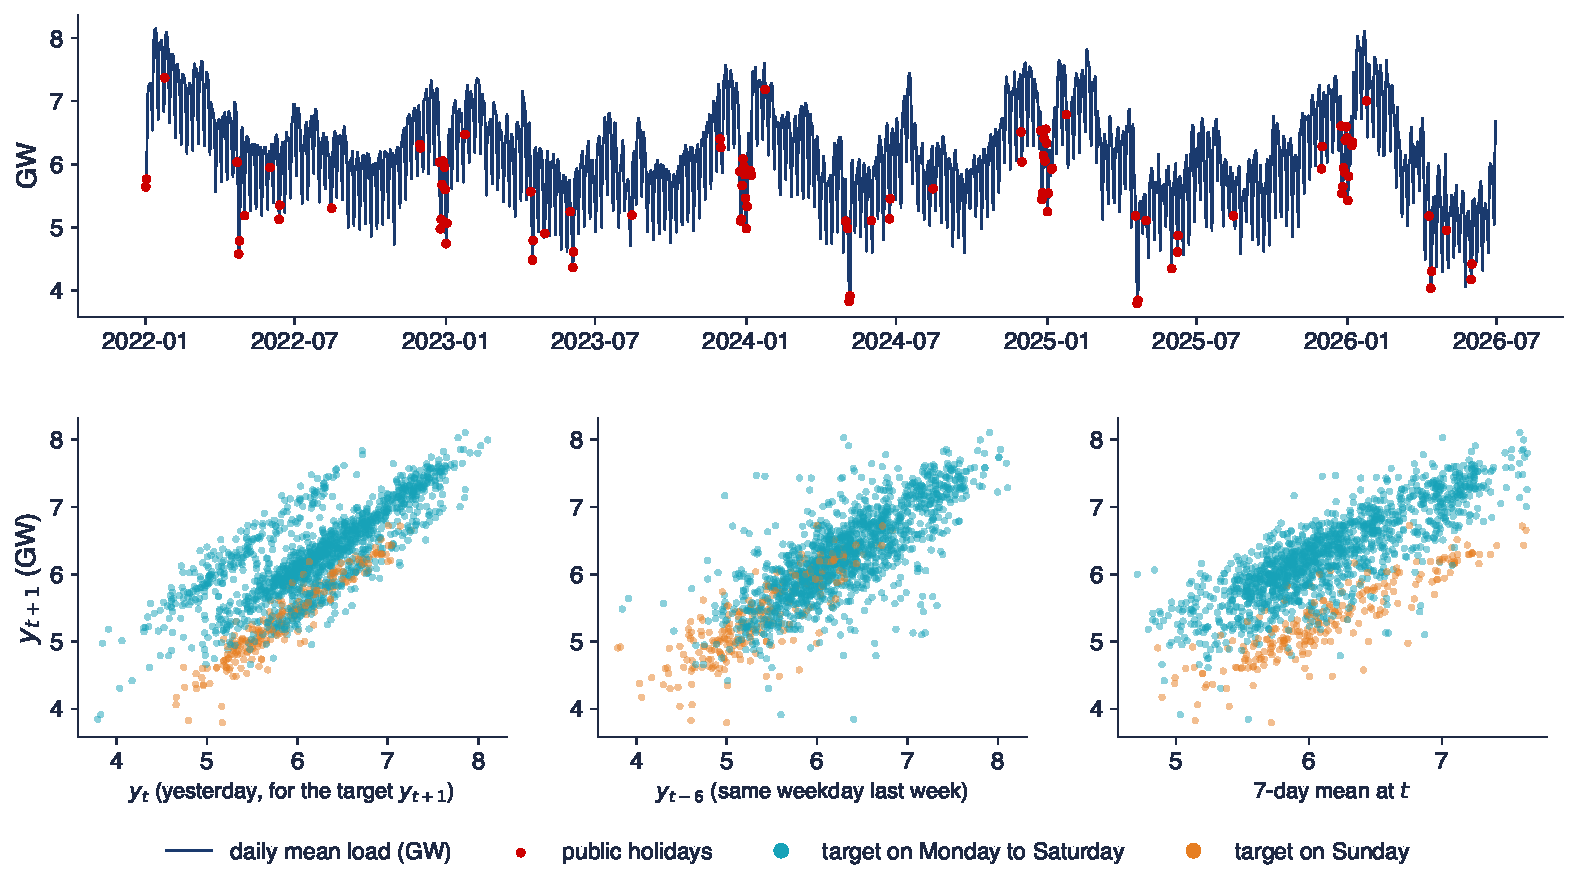
\includegraphics[width=0.97\textwidth,height=0.56\textheight,keepaspectratio]{tsa_ch9_features.pdf}
\end{center}
\vspace{-0.25cm}
\begin{itemize}
    \item Daily mean load of Romania, ENTSO-E (the European Network of Transmission System Operators for Electricity), 1 January 2022--30 June 2026, 1\,642 days; bottom: tomorrow's load against three features
\end{itemize}
\quantlet{TSA\_ch9\_supervised\_learning}{\qlurl{TSA_ch9_supervised_learning}}
\end{frame}

\begin{frame}{Interpreting the load features}
\itemsize{\small}
\begin{itemize}
    \item Mean 6.18 GW; minimum 3.79 GW on 20 April 2025 (Orthodox Easter), maximum 8.15 GW on 13 January 2022 (a winter week)
    \begin{itemize}
        \item weekly cycle, annual cycle (winter heating, summer cooling) and deep holiday dips: the multiple seasonality of \tsachlink{https://danpele.github.io/Time-Series-Analysis/EN/Courses/chapter4_seasonality_forecasting.pdf}{Chapter 4}
    \end{itemize}
    \item Correlation with tomorrow's load: $y_t$ 0.77; the same weekday last week 0.82; the 7-day mean 0.74
    \begin{itemize}
        \item with $y_t$ alone the Sundays form a separate cloud: a single linear lag cannot represent the weekly pattern
        \item the table used below has 1\,614 rows and 30 features (14 lags, two means, the same weekday, calendar)
    \end{itemize}
\end{itemize}
\end{frame}

\begin{frame}{Multi-step forecasts: three strategies}
\itemsize{\small}
\begin{itemize}
    \item \textbf{Recursive} (iterated): one model for $h = 1$; its forecast replaces the unknown $y_{T+1}$ and the model is applied again
    \begin{itemize}
        \item this is how ARIMA forecasts (\tsachlink{https://danpele.github.io/Time-Series-Analysis/EN/Courses/chapter3_unit_roots_arima_models.pdf}{Chapter 3}); errors accumulate when the one-step model is wrong
    \end{itemize}
    \item \textbf{Direct}: a separate model $\hat f_h$ for each horizon $h = 1, \dots, H$, trained on the target $y_{t+h}$
    \begin{itemize}
        \item no error accumulation, but $H$ models and fewer rows for long horizons; the forecasts of different $h$ need not be coherent
    \end{itemize}
    \item \textbf{Multi-output} (MIMO, multiple-input multiple-output): one model returns the vector $(\hat y_{T+1}, \dots, \hat y_{T+H})$
    \begin{itemize}
        \item natural for neural networks; review and comparison: \refBenTaieb
    \end{itemize}
\end{itemize}
\end{frame}

\begin{frame}{Recursive, direct and multi-output forecasts}
\itemsize{\footnotesize}
\begin{center}
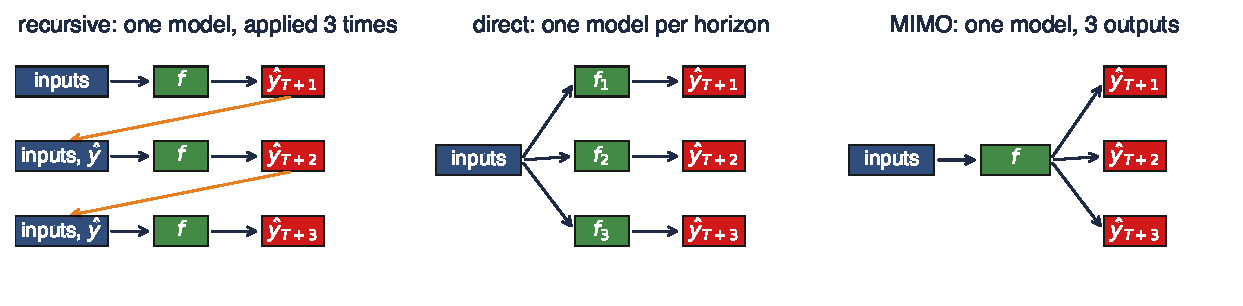
\includegraphics[width=0.97\textwidth,height=0.45\textheight,keepaspectratio]{tsa_ch9_strategies.pdf}
\end{center}
\vspace{-0.25cm}
\begin{itemize}
    \item Blue: the inputs known at the origin $T$; green: the fitted models; red: the forecasts; orange: a forecast fed back as an input
\end{itemize}
\quantlet{TSA\_ch9\_supervised\_learning}{\qlurl{TSA_ch9_supervised_learning}}
\end{frame}

\begin{frame}{Worked example: recursive and direct two-step forecasts}
\itemsize{\small}
\begin{itemize}
    \item One-step model estimated on the table: $\hat y_{t+1} = 1.2 + 0.8\,y_t$; last value $y_T = 5$
    \begin{itemize}
        \item recursive: $\hat y_{T+1} = 1.2 + 0.8 \cdot 5 = 5.20$; \quad $\hat y_{T+2} = 1.2 + 0.8 \cdot 5.20 = 5.36$
        \item implied two-step rule: $\hat y_{T+2} = 2.16 + 0.64\,y_T$
    \end{itemize}
    \item Direct model estimated on the target $y_{t+2}$: $\hat y_{t+2} = 2.3 + 0.6\,y_t$; \quad $\hat y_{T+2} = 5.30$
    \begin{itemize}
        \item if the AR(1) were the true model, the direct coefficients would estimate the same $2.16$ and $0.64$
        \item they differ: the one-step model is misspecified at two steps (for example, a weekly pattern), and the direct model adapts to the horizon
    \end{itemize}
    \item Neither strategy wins always: try both on the validation data
\end{itemize}
\end{frame}

\begin{frame}{Recap: Forecasting as supervised learning}
\itemsize{\small}
\begin{itemize}
    \item A forecast is a prediction of $y_{t+h}$ from features known at $t$: lags, rolling statistics, calendar
    \item An AR$(p)$ is linear regression on lags; ML changes the function, not the table
    \item Multi-step: recursive (one model, iterated), direct (one model per $h$), MIMO (one model, $H$ outputs)
\end{itemize}
\end{frame}


%=============================================================================
\section{Validation without leakage}
%=============================================================================

\begin{frame}{Training, validation and test samples}
\itemsize{\small}
\begin{itemize}
    \item \textbf{Training} sample: estimates the parameters; \textbf{validation}: chooses the hyperparameters; \textbf{test}: measures the final accuracy, used once
    \begin{itemize}
        \item for time series the three samples are consecutive blocks, in this order
    \end{itemize}
    \item \textbf{Walk-forward} validation (time-series cross-validation, \tsachlink{https://danpele.github.io/Time-Series-Analysis/EN/Courses/chapter4_seasonality_forecasting.pdf}{Chapter 4}): train on data up to an origin, forecast the next block, move the origin forward
    \begin{itemize}
        \item \textbf{expanding} window: all past data; \textbf{rolling} window: the last $W$ observations (adapts to change, uses less data)
        \item the errors of all origins are pooled into MAE, RMSE, MASE (\tsachlink{https://danpele.github.io/Time-Series-Analysis/EN/Courses/chapter0_introduction.pdf}{Chapter 0}) and compared with the Diebold--Mariano test
    \end{itemize}
    \item Random $K$-fold cross-validation (random folds) is valid only for pure autoregressions with white-noise errors \refBHK
\end{itemize}
\end{frame}

\begin{frame}{Four validation schemes}
\itemsize{\footnotesize}
\begin{center}
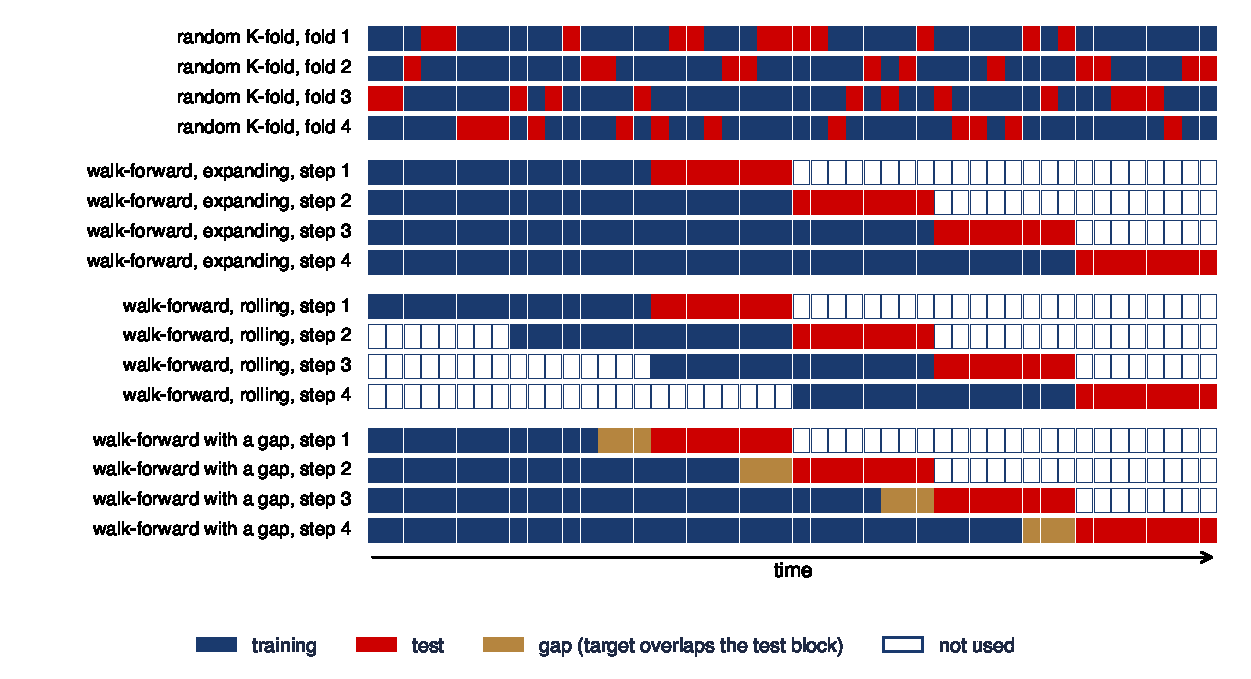
\includegraphics[width=0.97\textwidth,height=0.56\textheight,keepaspectratio]{tsa_ch9_cv_schemes.pdf}
\end{center}
\vspace{-0.25cm}
\begin{itemize}
    \item Random $K$-fold mixes past and future; walk-forward keeps the order; a gap removes the training rows whose targets overlap the test block
\end{itemize}
\quantlet{TSA\_ch9\_validation}{\qlurl{TSA_ch9_validation}}
\end{frame}

\begin{frame}{Look-ahead bias and leakage}
\itemsize{\small}
\begin{itemize}
    \item \textbf{Leakage}: information that would not be available at the forecast origin enters training or the features \refKaufman
    \begin{itemize}
        \item result: excellent validation scores that disappear in real use; \textbf{look-ahead bias} is its name in finance
    \end{itemize}
    \item Typical sources
    \begin{itemize}
        \item a rolling mean or a difference that includes $y_{t+1}$; centred moving averages and two-sided filters (\tsachlink{https://danpele.github.io/Time-Series-Analysis/EN/Courses/chapter0_introduction.pdf}{Chapter 0})
        \item scaling, imputation or feature selection fitted on the whole sample before the split
        \item overlapping targets (sums over the next $h$ days) with random folds or without a gap
        \item revised macro data: today's GDP vintage was not known at the origin; actual weather instead of the weather forecast
    \end{itemize}
    \item Rule: write the feature code as a function of the data up to $t$ only, and refit every preprocessing step inside each training window
\end{itemize}
\end{frame}

\begin{frame}{Leakage in practice: random folds on overlapping targets}
\itemsize{\footnotesize}
\begin{center}
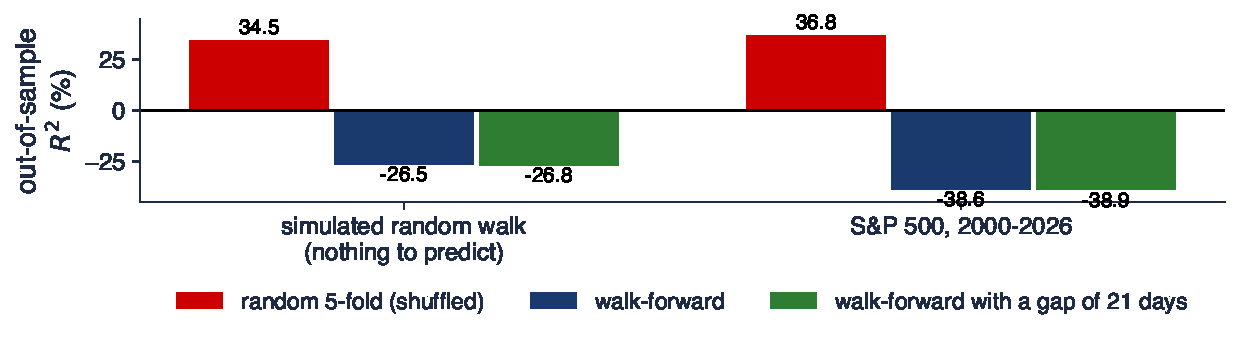
\includegraphics[width=0.97\textwidth,height=0.5\textheight,keepaspectratio]{tsa_ch9_leakage.pdf}
\end{center}
\vspace{-0.25cm}
\begin{itemize}
    \item Random forest for the sum of the next 21 daily returns; features: past sums over 5, 21, 63 days and volatilities; left: a simulated random walk; right: the S\&P 500, 6\,631 days
\end{itemize}
\quantlet{TSA\_ch9\_validation}{\qlurl{TSA_ch9_validation}}
\end{frame}

\begin{frame}{Interpreting the leakage experiment}
\itemsize{\small}
\begin{itemize}
    \item Random 5-fold reports $R^2$ = 34.5\% for a random walk, where nothing is predictable, and 36.8\% for the S\&P 500
    \begin{itemize}
        \item neighbouring targets share 20 of 21 returns: a test row has its near-copies in the training folds
    \end{itemize}
    \item Walk-forward: $-$26.5\% and $-$38.6\%; with a 21-day gap: $-$26.8\% and $-$38.9\%
    \begin{itemize}
        \item negative out-of-sample $R^2$: the forest is worse than the historical mean, as expected for returns (\tsachlink{https://danpele.github.io/Time-Series-Analysis/EN/Courses/chapter1_stochastic_processes_stationarity.pdf}{Chapter 1})
    \end{itemize}
    \item A model is only as good as its validation; a spectacular score is a reason to look for a leak
\end{itemize}
\end{frame}

\begin{frame}{Overfitting and the bias--variance trade-off}
\itemsize{\small}
\begin{itemize}
    \item Model $y = f(x) + \varepsilon$, $\Var(\varepsilon) = \sigma^2$; $\hat f$ estimated on a random training sample
    \begin{itemize}
        \item the expected test error at a point $x_0$:
        \item $E[(y_0 - \hat f(x_0))^2] = \underbrace{(E[\hat f(x_0)] - f(x_0))^2}_{\text{bias}^2} + \underbrace{\Var(\hat f(x_0))}_{\text{variance}} + \sigma^2$
        \item $f$: the true function; $y_0$: a new observation at $x_0$; the expectation is over training samples and noise; $\sigma^2$: the noise that no model can remove
    \end{itemize}
    \item \textbf{Overfitting}: a flexible model learns the noise; small training error, large test error
    \begin{itemize}
        \item \textbf{underfitting}: a rigid model misses the signal (large bias)
    \end{itemize}
    \item Every ML method has a complexity knob (depth, number of trees, penalty, hidden units); validation sets it
\end{itemize}
\end{frame}

\begin{frame}{Bias and variance of regression trees}
\itemsize{\footnotesize}
\begin{center}
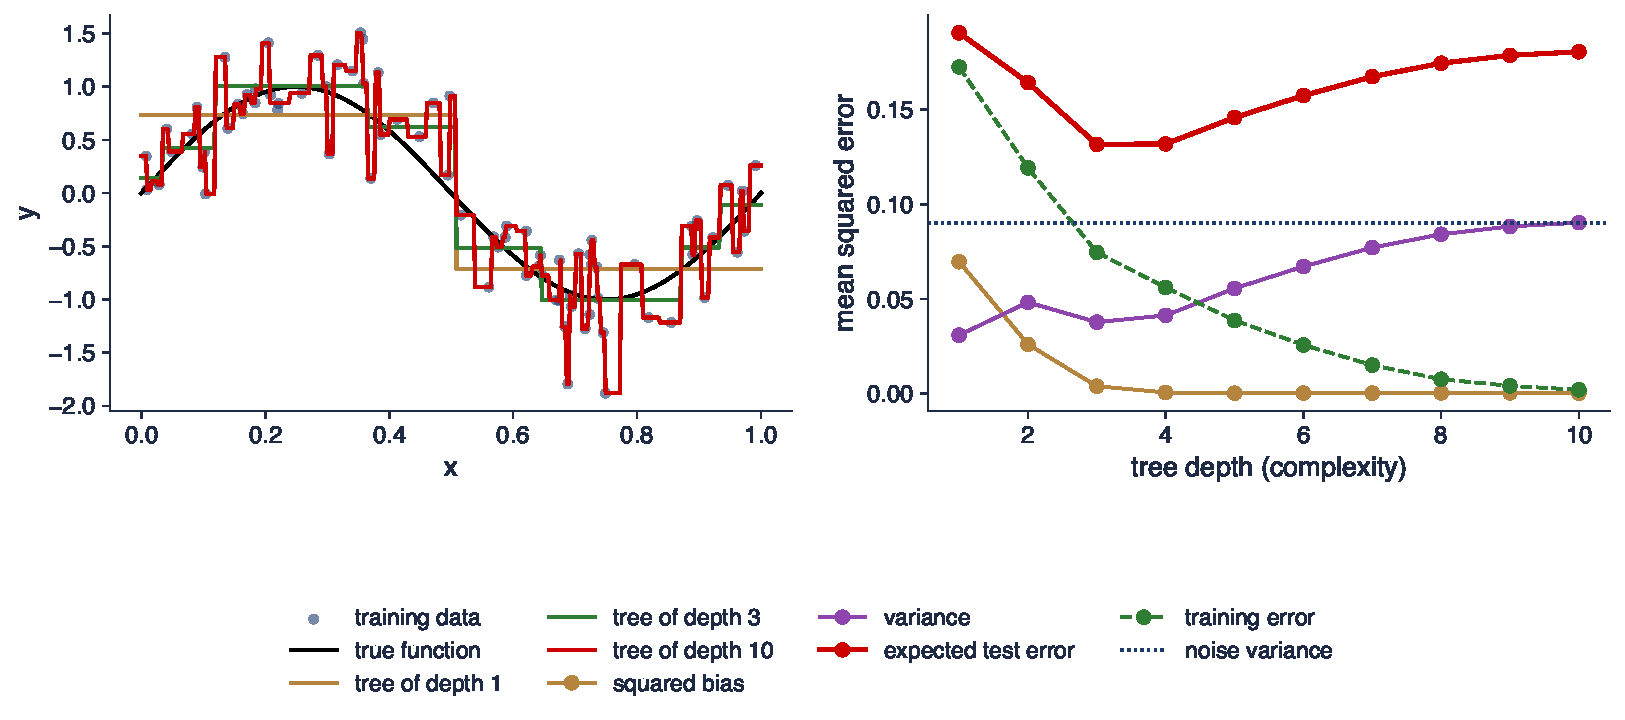
\includegraphics[width=0.97\textwidth,height=0.52\textheight,keepaspectratio]{tsa_ch9_bias_variance.pdf}
\end{center}
\vspace{-0.25cm}
\begin{itemize}
    \item Simulation: $y = \sin(2\pi x) + \varepsilon$, $\sigma = 0.3$, 80 points, 300 training samples; trees of depth 1 to 10
\end{itemize}
\quantlet{TSA\_ch9\_validation}{\qlurl{TSA_ch9_validation}}
\end{frame}

\begin{frame}{Interpreting the U-shaped test error}
\itemsize{\small}
\begin{itemize}
    \item Depth 1: bias$^2$ 0.070, variance 0.031; depth 10: bias$^2$ 0.000, variance 0.090
    \begin{itemize}
        \item the expected test error is smallest at depth 3 (0.132), above the noise variance 0.09
    \end{itemize}
    \item The training error falls to 0.002 at depth 10: it cannot choose the complexity
    \item Ensembles (random forest, boosting) and penalties (ridge, lasso) reduce the variance without losing much bias
\end{itemize}
\end{frame}

\begin{frame}{Recap: Validation without leakage}
\itemsize{\small}
\begin{itemize}
    \item Walk-forward: train on the past, test on the next block, move on; random folds only for pure autoregressions
    \item Leakage: future values in features, preprocessing on the full sample, overlapping targets, revised data
    \item Test error = bias$^2$ + variance + noise; validation sets the complexity
\end{itemize}
\end{frame}


%=============================================================================
\section{Regularised linear models: ridge and lasso}
%=============================================================================

\begin{frame}{Many lags, unstable least squares}
\itemsize{\small}
\begin{itemize}
    \item Linear model on $p$ standardised features: $\hat y = \beta_0 + \sum_j \beta_j x_j$; OLS (ordinary least squares) minimises $\sum_t (y_t - \hat y_t)^2$
    \begin{itemize}
        \item neighbouring lags are highly correlated: OLS coefficients become large, of opposite signs and unstable from one window to the next
    \end{itemize}
    \item \textbf{Standardise} first: $x_j \to (x_j - \bar x_j)/s_j$, with $\bar x_j$, $s_j$ from the training window only
    \begin{itemize}
        \item otherwise the penalty treats features measured in GW and in dummies unequally
    \end{itemize}
    \item Idea of regularisation: accept a little bias in exchange for a large fall in variance
\end{itemize}
\end{frame}

\begin{frame}{Ridge and lasso}
\itemsize{\footnotesize}
\begin{itemize}
    \item \textbf{Ridge} \refHoerlK: $\min_{\beta} \sum_t (y_t - \beta_0 - \mathbf{x}_t'\beta)^2 + \lambda\sum_j \beta_j^2$
    \begin{itemize}
        \item $\lambda \ge 0$: the penalty ($\lambda = 0$: OLS); $\mathbf{X}$: the matrix of standardised features; $\mathbf{y}$: the targets; $\mathbf{I}$: the identity matrix
        \item closed form $\hat\beta = (\mathbf{X}'\mathbf{X} + \lambda\mathbf{I})^{-1}\mathbf{X}'\mathbf{y}$; all coefficients shrink towards 0, none becomes exactly 0
    \end{itemize}
    \item \textbf{Lasso} \refTib\ (least absolute shrinkage and selection operator): penalty $\lambda\sum_j |\beta_j|$
    \begin{itemize}
        \item sets some coefficients exactly to 0: it selects lags
    \end{itemize}
    \item \textbf{Worked example}, one standardised feature, $S_{xy} = \sum x_ty_t = 90$, $S_{xx} = \sum x_t^2 = 100$
    \begin{itemize}
        \item OLS $90/100 = 0.90$; ridge, $\lambda = 50$: $90/150 = 0.60$; lasso, $\lambda = 40$: $(90 - 20)/100 = 0.70$; lasso, $\lambda \ge 180$: exactly 0
        \item lasso in one dimension: $\hat\beta = \mathrm{sign}(S_{xy})\max(|S_{xy}| - \lambda/2, 0)/S_{xx}$ (soft thresholding)
    \end{itemize}
    \item $\lambda$ is chosen by walk-forward validation (\texttt{TimeSeriesSplit}), never by random folds
\end{itemize}
\end{frame}

\begin{frame}{Ridge and lasso paths on the load features}
\itemsize{\footnotesize}
\begin{center}
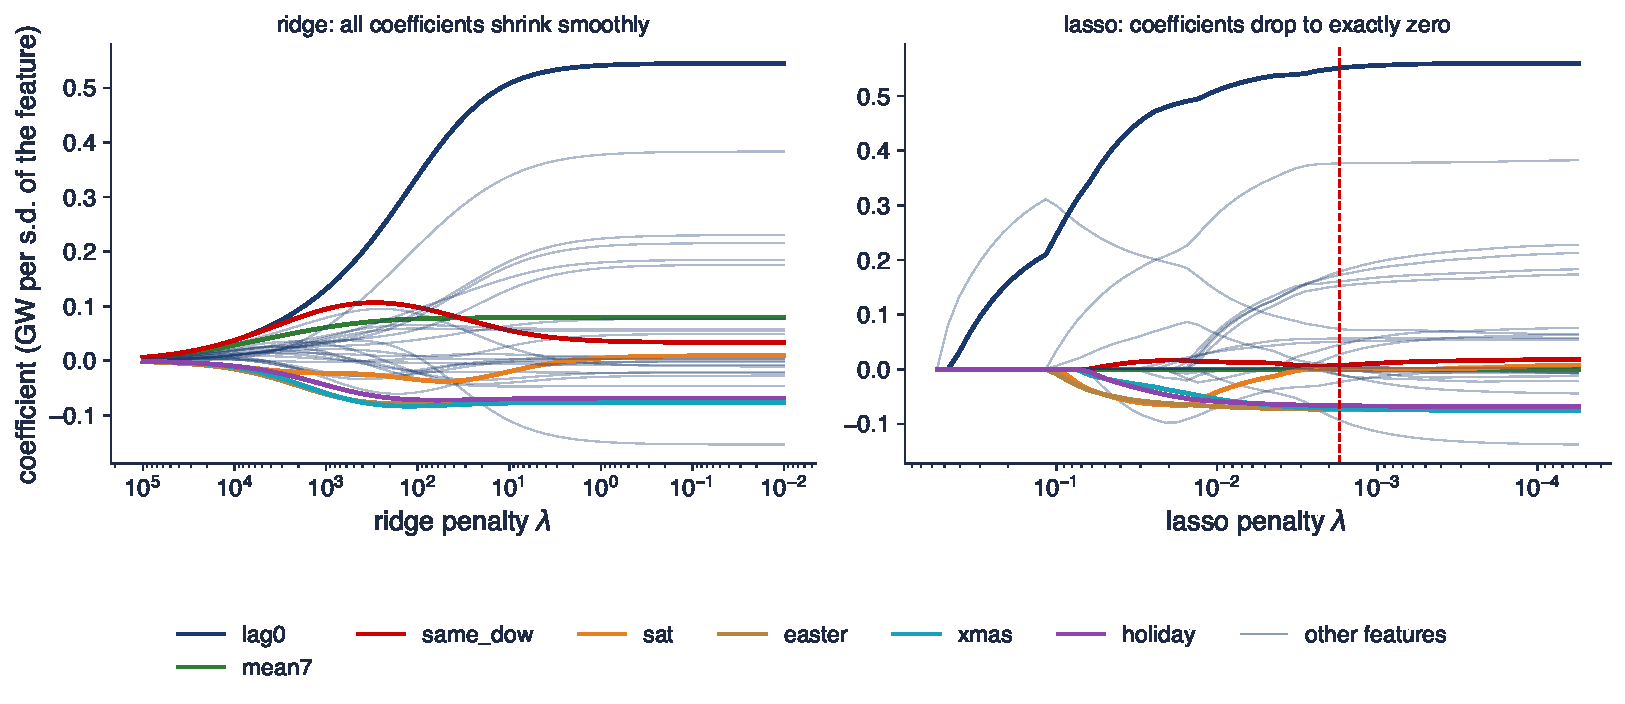
\includegraphics[width=0.97\textwidth,height=0.54\textheight,keepaspectratio]{tsa_ch9_shrinkage.pdf}
\end{center}
\vspace{-0.25cm}
\begin{itemize}
    \item Target: tomorrow's load; 30 standardised features; data up to 30 June 2025 (1\,249 rows); dashed: the lasso penalty chosen by walk-forward cross-validation
\end{itemize}
\quantlet{TSA\_ch9\_regularisation\_trees}{\qlurl{TSA_ch9_regularisation_trees}}
\end{frame}

\begin{frame}{Interpreting the coefficient paths}
\itemsize{\small}
\begin{itemize}
    \item With a large penalty all coefficients are near 0; as $\lambda$ falls, $y_t$ (lag0) enters first and dominates, with coefficient 0.55 GW per standard deviation
    \begin{itemize}
        \item then the weekday dummies and the holiday flags: the calendar carries most of the remaining signal
    \end{itemize}
    \item At the chosen penalty the lasso keeps 22 of 30 features: many lags are redundant once $y_t$, the weekday and the holidays are in
    \item Ridge keeps everything but shrinks it smoothly; on the test origins of Section 6 ridge is the best ML model
\end{itemize}
\end{frame}

\begin{frame}{Recap: Ridge and lasso}
\itemsize{\small}
\begin{itemize}
    \item Penalised least squares: ridge $\lambda\sum\beta_j^2$ shrinks; lasso $\lambda\sum|\beta_j|$ shrinks and selects
    \item Standardise inside each training window; choose $\lambda$ walk-forward
    \item A regularised AR with calendar dummies is a strong ML baseline
\end{itemize}
\end{frame}


%=============================================================================
\section{Trees, random forest and gradient boosting}
%=============================================================================

\begin{frame}{Regression trees}
\itemsize{\small}
\begin{itemize}
    \item A \textbf{regression tree} splits the feature space with questions ``$x_j \le c$?'' and predicts, in each final region (leaf), the mean target of its training rows
    \begin{itemize}
        \item the split is chosen greedily: the $(j, c)$ with the smallest sum of squared errors of the two children
    \end{itemize}
    \item Strengths: nonlinearity and interactions (weekday $\times$ season) without specifying them; no scaling needed
    \begin{itemize}
        \item weaknesses: a single tree is unstable (high variance) and piecewise constant
    \end{itemize}
    \item \textbf{A tree cannot extrapolate}: its forecast is always a mean of training targets
    \begin{itemize}
        \item for trending series: model differences, growth rates or the deviation from a trend, not levels
    \end{itemize}
\end{itemize}
\end{frame}

\begin{frame}{A depth-2 tree for tomorrow's load}
\itemsize{\footnotesize}
\begin{center}
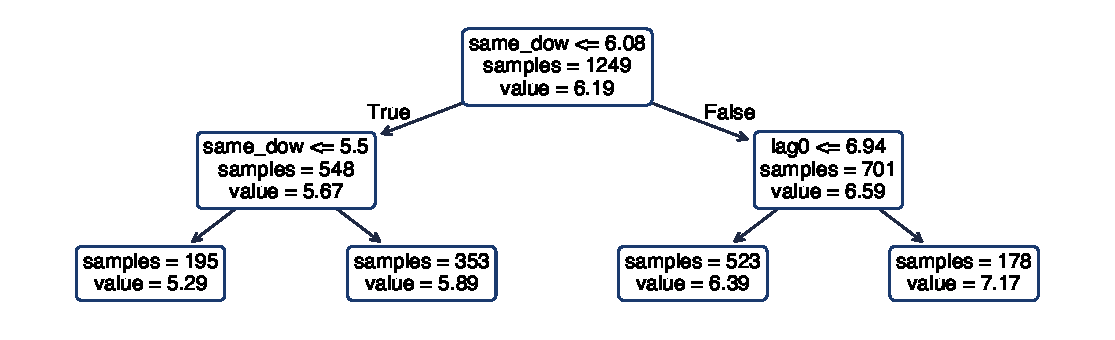
\includegraphics[width=0.97\textwidth,height=0.5\textheight,keepaspectratio]{tsa_ch9_tree.pdf}
\end{center}
\vspace{-0.25cm}
\begin{itemize}
    \item Features: $y_t$ (lag0), the same weekday last week (same\_dow), weekend and holiday flags; data up to 30 June 2025; at least 20 days per leaf
\end{itemize}
\quantlet{TSA\_ch9\_regularisation\_trees}{\qlurl{TSA_ch9_regularisation_trees}}
\end{frame}

\begin{frame}{Interpreting the tree}
\itemsize{\small}
\begin{itemize}
    \item First question: was the same weekday last week below 6.08 GW? It separates weekends and holidays from working days
    \begin{itemize}
        \item four leaves: 5.29, 5.89, 6.39 and 7.17 GW, with 195, 353, 523 and 178 days
    \end{itemize}
    \item Four numbers already explain $R^2$ = 0.64 of the variance in training; deeper trees add detail and variance
    \item The forecast for any day is one of these four means: a tree never forecasts outside the range of the training targets
\end{itemize}
\end{frame}

\begin{frame}{Random forest}
\itemsize{\small}
\begin{itemize}
    \item \textbf{Bagging} (bootstrap aggregation): grow $B$ deep trees on bootstrap samples of the rows and average them
    \begin{itemize}
        \item averaging $B$ trees with correlation $\rho$ and variance $\sigma^2$ gives variance $\rho\sigma^2 + (1 - \rho)\sigma^2/B$
    \end{itemize}
    \item \textbf{Random forest} \refBreiman: at each split, only a random subset of features is tried (\texttt{max\_features})
    \begin{itemize}
        \item this decorrelates the trees ($\rho$ falls), so the average has a lower variance
    \end{itemize}
    \item Hyperparameters: number of trees (more is never worse, only slower), \texttt{max\_features}, minimum leaf size
    \begin{itemize}
        \item the bootstrap ignores time order inside the training window; that is fine, because the validation is walk-forward
    \end{itemize}
\end{itemize}
\end{frame}

\begin{frame}{Gradient boosting}
\itemsize{\footnotesize}
\begin{itemize}
    \item \textbf{Boosting} \refFriedman: add small trees one at a time, each fitted to the residuals (the negative gradient of the loss) of the current model
    \begin{itemize}
        \item $F_m(\mathbf{x}) = F_{m-1}(\mathbf{x}) + \nu\,g_m(\mathbf{x})$; $F_m$: the model after $m$ trees; $g_m$: the $m$-th small tree; $\nu$: the \textbf{learning rate} (0.01--0.3)
    \end{itemize}
    \item \textbf{Worked example}: targets $5, 6, 8$; start with the mean $F_0 = 6.33$; residuals $-$1.33, $-$0.33, +1.67
    \begin{itemize}
        \item a stump that isolates the third point predicts $1.67$ there; with $\nu = 0.1$: $F_1 = 6.33 + 0.1 \cdot 1.67 = 6.500$
    \end{itemize}
    \item Fast implementations bin the features into histograms: XGBoost \refXGB, LightGBM \refLGBM, \texttt{HistGradientBoostingRegressor} in scikit-learn
    \begin{itemize}
        \item below we write GB for gradient boosting; the winners of M5 (Section 10) used LightGBM
        \item hyperparameters: number of trees with \textbf{early stopping} on validation data, tree size, $\nu$, minimum leaf size
    \end{itemize}
\end{itemize}
\end{frame}

\begin{frame}{One tree, a forest and boosting on the load}
\itemsize{\footnotesize}
\begin{center}
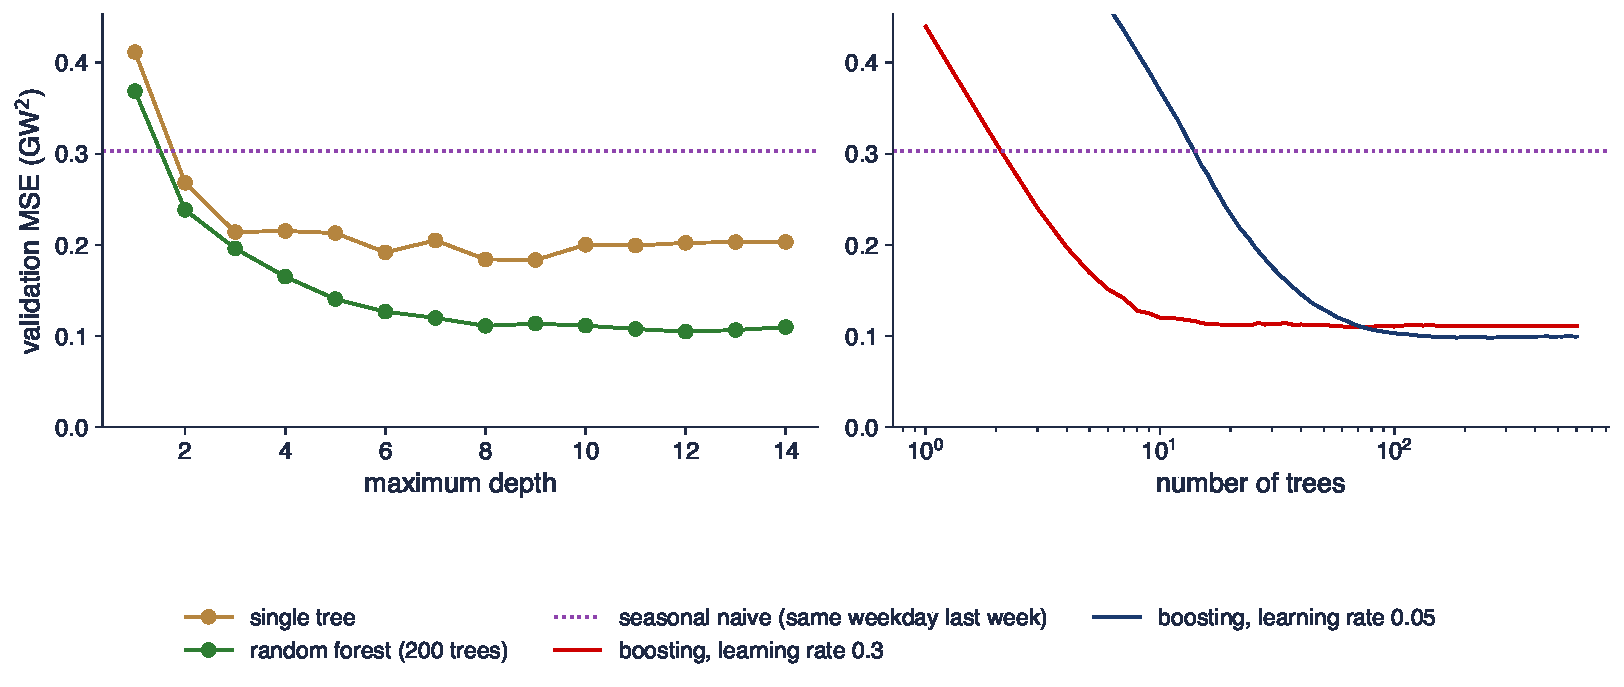
\includegraphics[width=0.97\textwidth,height=0.5\textheight,keepaspectratio]{tsa_ch9_ensembles.pdf}
\end{center}
\vspace{-0.25cm}
\begin{itemize}
    \item Tomorrow's load; training up to 31 December 2024 (1069 days), validation January--June 2025 (180 days); dotted: the seasonal naive forecast
\end{itemize}
\quantlet{TSA\_ch9\_regularisation\_trees}{\qlurl{TSA_ch9_regularisation_trees}}
\end{frame}

\begin{frame}{Interpreting the ensembles}
\itemsize{\small}
\begin{itemize}
    \item Single tree: best validation MSE (mean squared error) 0.183 at depth 9; random forest: 0.105 at depth 12
    \begin{itemize}
        \item averaging removes most of the variance; the seasonal naive forecast has 0.303
    \end{itemize}
    \item Boosting with $\nu = 0.3$: minimum 0.110 after 72 trees; with $\nu = 0.05$: 0.098 after 256 trees
    \begin{itemize}
        \item a small learning rate needs more trees and usually ends slightly lower; early stopping picks the number of trees
    \end{itemize}
\end{itemize}
\end{frame}

\begin{frame}{Trees cannot extrapolate: the Romanian price level}
\itemsize{\footnotesize}
\begin{center}
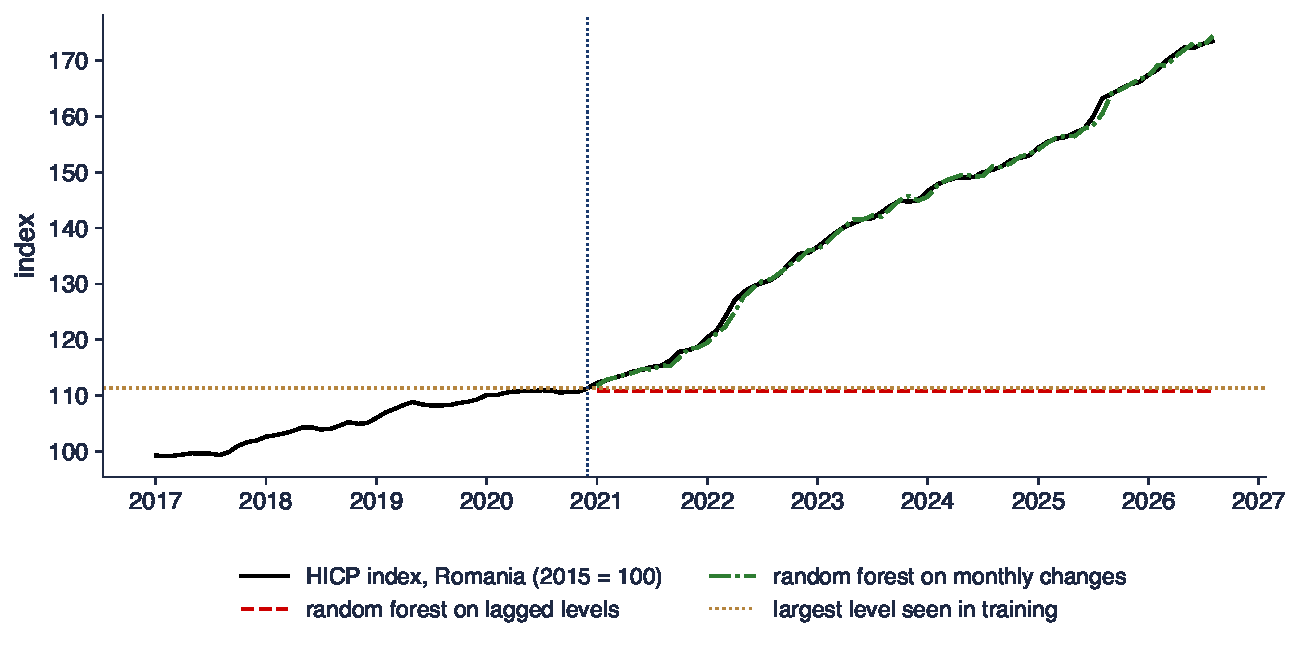
\includegraphics[width=0.97\textwidth,height=0.5\textheight,keepaspectratio]{tsa_ch9_extrapolation.pdf}
\end{center}
\vspace{-0.25cm}
\begin{itemize}
    \item HICP (harmonised index of consumer prices) of Romania, Eurostat, 2015 = 100; one-month-ahead forecasts from random forests trained up to December 2020, on lagged levels or on monthly log changes
\end{itemize}
\quantlet{TSA\_ch9\_regularisation\_trees}{\qlurl{TSA_ch9_regularisation_trees}}
\end{frame}

\begin{frame}{Interpreting the extrapolation failure}
\itemsize{\small}
\begin{itemize}
    \item The highest index in training was 111.3; by August 2026 the index reached 173.4
    \begin{itemize}
        \item the forest on levels stays near 110.8 for five years: RMSE 36.9 index points
    \end{itemize}
    \item The same forest on monthly changes, then cumulated, follows the index: RMSE 0.71
    \item \tsachlink{https://danpele.github.io/Time-Series-Analysis/EN/Courses/chapter3_unit_roots_arima_models.pdf}{Chapter 3} again: difference or transform non-stationary series before a tree sees them
\end{itemize}
\end{frame}

\begin{frame}{The features a model uses}
\itemsize{\small}
\begin{itemize}
    \item \textbf{Permutation importance}: shuffle one feature in the test data and measure how much the error grows
    \begin{itemize}
        \item model-agnostic; measured out of sample; correlated features share (and hide) their importance
    \end{itemize}
    \item Impurity-based importance of trees (MDI, mean decrease impurity) is computed in training and favours continuous features: prefer permutation
    \item Importance is not causality: it describes the model, not the electricity system
\end{itemize}
\end{frame}

\begin{frame}{Permutation importance of gradient boosting}
\itemsize{\footnotesize}
\begin{center}
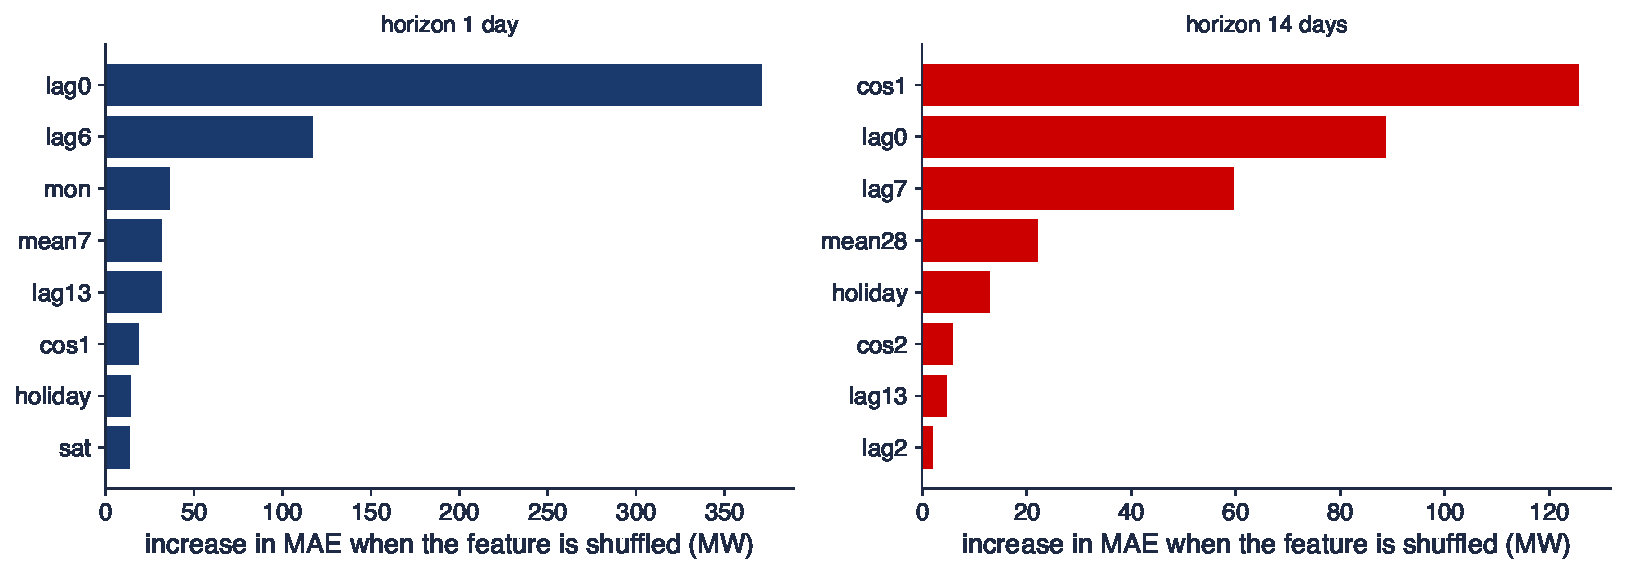
\includegraphics[width=0.97\textwidth,height=0.5\textheight,keepaspectratio]{tsa_ch9_importance.pdf}
\end{center}
\vspace{-0.25cm}
\begin{itemize}
    \item Direct GB models for horizons 1 and 14 days; trained up to 31 December 2024, evaluated on January--June 2025; 20 random permutations per feature
\end{itemize}
\quantlet{TSA\_ch9\_load\_forecasting}{\qlurl{TSA_ch9_load_forecasting}}
\end{frame}

\begin{frame}{Interpreting the importances}
\itemsize{\small}
\begin{itemize}
    \item One day ahead: lag0 (+371 MW of MAE when shuffled) and lag6 (+117 MW) dominate
    \begin{itemize}
        \item yesterday and the same weekday last week: the persistence and the weekly cycle
    \end{itemize}
    \item Fourteen days ahead: cos1 (+126 MW) and lag0 (+89 MW)
    \begin{itemize}
        \item the annual cycle (cos1, the Fourier term) gains weight as the recent values become less informative
    \end{itemize}
\end{itemize}
\end{frame}

\begin{frame}{Recap: Trees and ensembles}
\itemsize{\small}
\begin{itemize}
    \item A tree is a piecewise-constant function found by greedy splits; it cannot extrapolate
    \item Random forest averages decorrelated deep trees (less variance); boosting adds small trees on residuals (less bias)
    \item GB (gradient boosting, LightGBM, XGBoost, \texttt{HistGradientBoosting}): learning rate, number of trees, early stopping
    \item Permutation importance measures what the model uses, out of sample
\end{itemize}
\end{frame}


%=============================================================================
\section{Neural networks}
%=============================================================================

\begin{frame}{The multilayer perceptron}
\itemsize{\footnotesize}
\begin{columns}[T]
\begin{column}{0.36\textwidth}
\centering
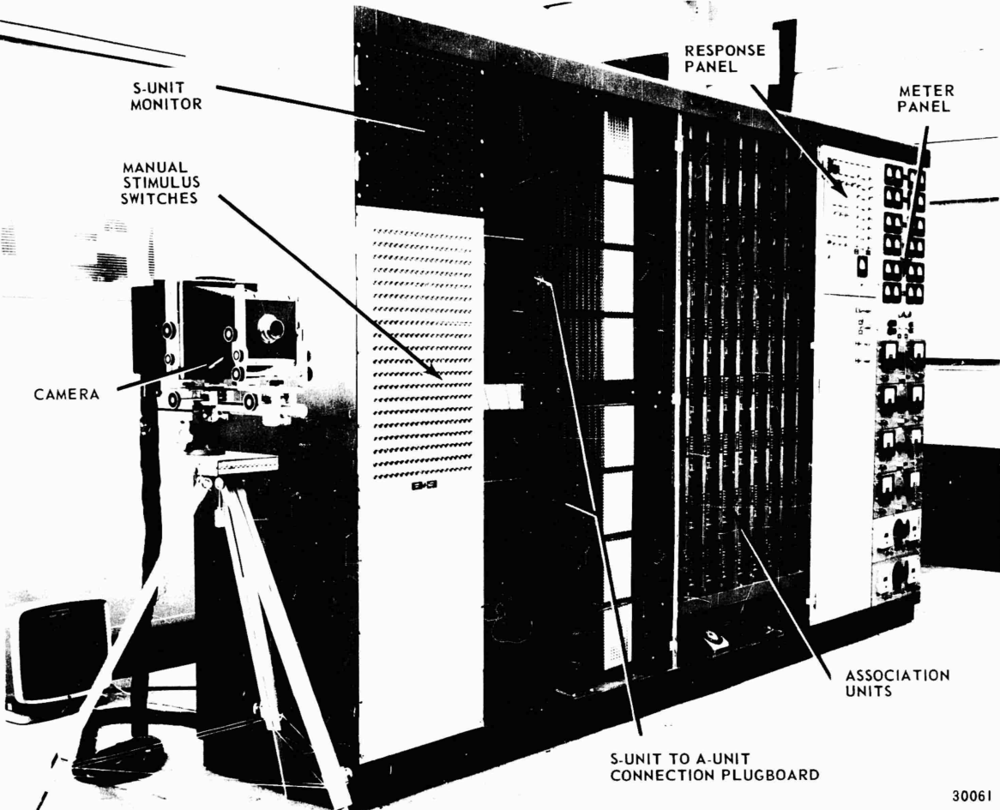
\includegraphics[height=0.5\textheight]{ch9_mark1_perceptron_1960.png}\\[1mm]
\imgcap{Mark I Perceptron, Cornell (1960): the first trainable neural network, built in hardware}
\imgcredit{https://commons.wikimedia.org/wiki/File:Mark_I_Perceptron,_Figure_2_of_operator\%27s_manual.png}{Image: J. C. Hay, A. E. Murray (1960), Mark I Perceptron operator's manual; public domain; Wikimedia Commons}
\end{column}
\begin{column}{0.62\textwidth}
\begin{itemize}
    \item \textbf{MLP} (multilayer perceptron), one hidden layer with $q$ neurons:
    \begin{itemize}
        \item $h_j = g(b_j + \mathbf{w}_j'\mathbf{x})$, $j = 1, \dots, q$; \quad $\hat y = c + \sum_j v_jh_j$
        \item $\mathbf{x}$: the inputs; $\mathbf{w}_j$, $b_j$: the weights and the bias of neuron $j$; $h_j$: its output; $v_j$, $c$: the output weights and constant
        \item $g$: activation function (ReLU $\max(0, z)$, tanh, logistic); with $g(z) = z$ the network is linear again
    \end{itemize}
    \item Universal approximation \refHornik: enough hidden neurons approximate any continuous function
    \begin{itemize}
        \item parameters: 3 inputs and 5 neurons already give $3 \cdot 5 + 5 + 5 + 1 = 26$ weights
    \end{itemize}
\end{itemize}
\end{column}
\end{columns}
\end{frame}

\begin{frame}{A small network and its activation functions}
\itemsize{\footnotesize}
\begin{center}
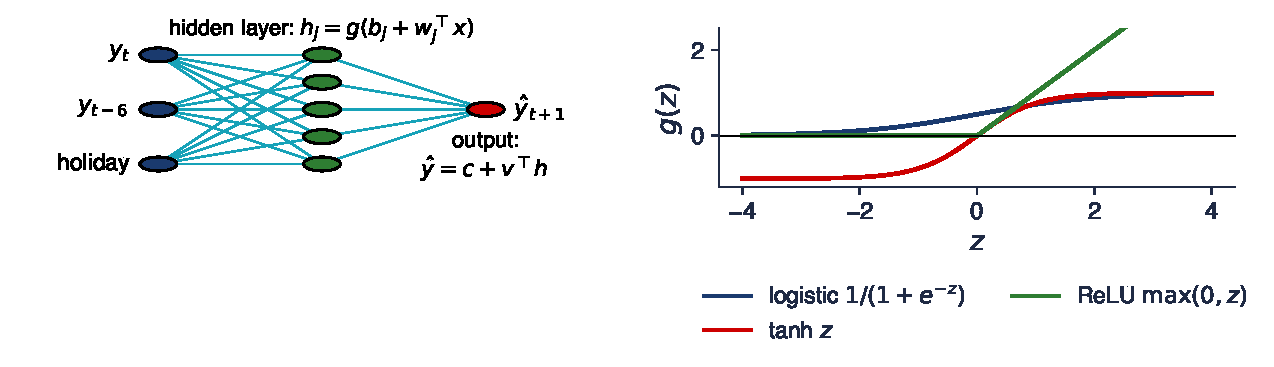
\includegraphics[width=0.97\textwidth,height=0.48\textheight,keepaspectratio]{tsa_ch9_mlp.pdf}
\end{center}
\vspace{-0.25cm}
\begin{itemize}
    \item Left: 3 inputs (yesterday, the same weekday last week, a holiday flag), 5 hidden neurons, one output; right: three activation functions
\end{itemize}
\quantlet{TSA\_ch9\_neural\_networks}{\qlurl{TSA_ch9_neural_networks}}
\end{frame}

\begin{frame}{Training a network}
\itemsize{\small}
\begin{itemize}
    \item Minimise the training loss by \textbf{gradient descent}; the gradients come from back-propagation \refRumelhart
    \begin{itemize}
        \item SGD (stochastic gradient descent) and Adam use small random batches; one pass through the data is an epoch
    \end{itemize}
    \item The loss surface has many local minima: results depend on the random starting weights
    \begin{itemize}
        \item fix the seed, and average a few networks with different seeds (an ensemble)
    \end{itemize}
    \item Regularisation: an L2 penalty on the weights, early stopping, dropout (randomly switching off neurons)
    \begin{itemize}
        \item inputs and targets must be standardised with training-window statistics
    \end{itemize}
    \item Small data (a few thousand rows) favour small networks; deep networks need many series or long high-frequency data
\end{itemize}
\end{frame}

\begin{frame}{Recurrent networks and the LSTM (1/2): the recurrent network}
\itemsize{\footnotesize}
\begin{itemize}
    \item \textbf{RNN} (recurrent neural network): a hidden state carries the past forward, with the same weights at every step
    \begin{itemize}
        \item $h_t = \tanh(Wh_{t-1} + Ux_t + b)$: the new state mixes the previous state and the new input
        \item $x_t$: the input at $t$; $h_t$: the hidden state; $W$, $U$, $b$: weights and bias, shared by all steps; $\tanh$ keeps each component in $(-1, 1)$
        \item the forecast is read from the last state, for example $\hat y_{t+1} = v'h_t + c$
    \end{itemize}
    \item The difficulty: training through many steps multiplies many derivatives
    \begin{itemize}
        \item the gradients vanish or explode: a plain RNN forgets what happened more than a few steps back
    \end{itemize}
    \item Honest summary \refHBB
    \begin{itemize}
        \item on single, short series, recurrent networks rarely beat ETS or ARIMA
        \item they shine with many related series and enough data (global models, \refDeepAR)
    \end{itemize}
\end{itemize}
\end{frame}

\begin{frame}{Recurrent networks and the LSTM (2/2): the LSTM cell}
\itemsize{\footnotesize}
\begin{itemize}
    \item \textbf{LSTM} (long short-term memory) \refLSTM: a cell state $c_t$ updated additively, controlled by three gates
    \begin{itemize}
        \item the gates: $f_t = \sigma(W_f[h_{t-1}, x_t] + b_f)$ (forget), $i_t = \sigma(W_i[h_{t-1}, x_t] + b_i)$ (input), $o_t = \sigma(W_o[h_{t-1}, x_t] + b_o)$ (output)
        \item the candidate new content: $\tilde c_t = \tanh(W_c[h_{t-1}, x_t] + b_c)$
        \item $\sigma(z) = 1/(1 + e^{-z}) \in (0, 1)$: the logistic function; $[h_{t-1}, x_t]$: the two vectors stacked; $W_f, W_i, W_o, W_c$ and $b_f, b_i, b_o, b_c$: weights and biases
    \end{itemize}
    \item The updates of the cell and of the output
    \begin{itemize}
        \item $c_t = f_t \odot c_{t-1} + i_t \odot \tilde c_t$: with $f_t$ close to 1 the old memory survives many steps; $i_t$ sets how much new content enters
        \item $h_t = o_t \odot \tanh(c_t)$: the output gate decides which part of the memory is passed on; $\odot$: element-wise product
    \end{itemize}
    \item Each gate is a small logistic layer: an LSTM with 32 units and 8 inputs has about 5\,400 weights
\end{itemize}
\end{frame}

\begin{frame}{A recurrent network and the LSTM cell}
\itemsize{\footnotesize}
\begin{center}
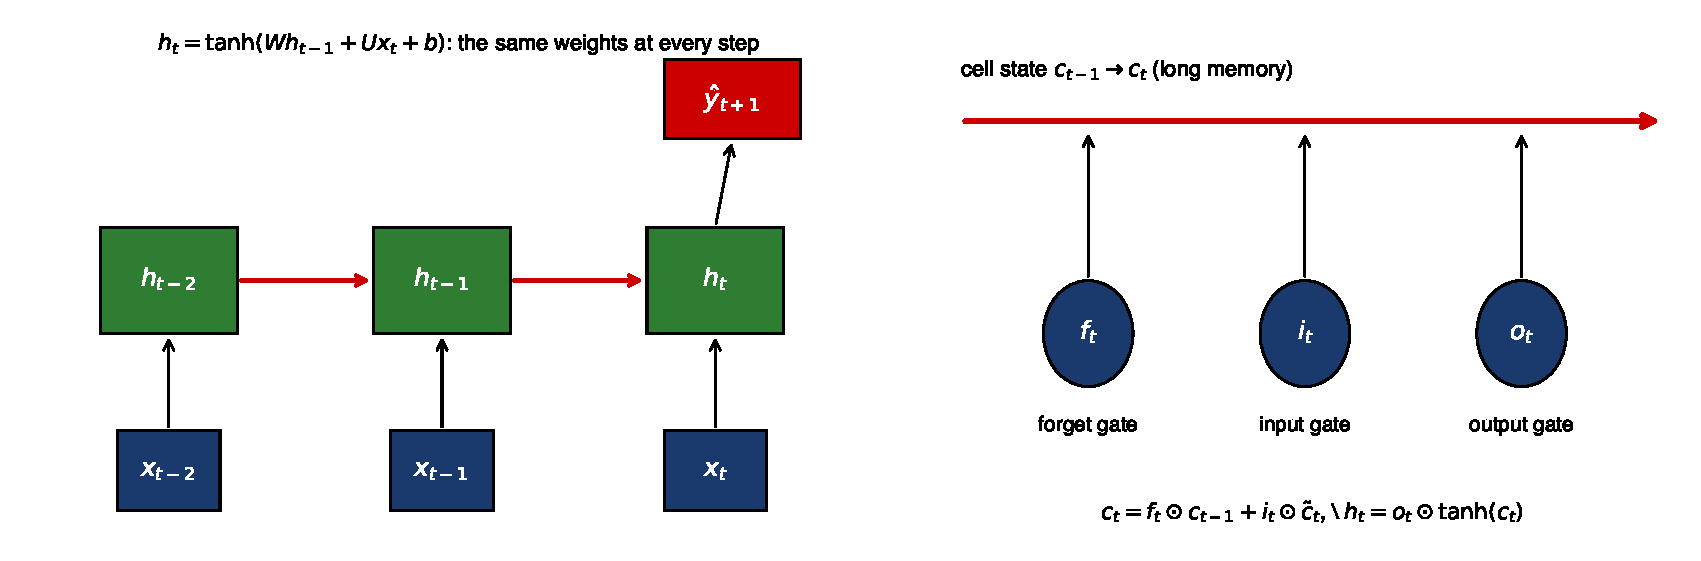
\includegraphics[width=0.97\textwidth,height=0.48\textheight,keepaspectratio]{tsa_ch9_rnn.pdf}
\end{center}
\vspace{-0.25cm}
\begin{itemize}
    \item Left: the RNN unrolled over three steps; right: the LSTM cell state (red) and its three gates; $\odot$: element-wise product
\end{itemize}
\quantlet{TSA\_ch9\_neural\_networks}{\qlurl{TSA_ch9_neural_networks}}
\end{frame}

\begin{frame}{Sepp Hochreiter and the LSTM}
\itemsize{\small}
\begin{columns}[T]
\begin{column}{0.38\textwidth}
\centering

\includegraphics[height=0.55\textheight]{ch9_sepp_hochreiter_2015.jpg}\\[1mm]
\imgcap{Sepp Hochreiter (2015), Johannes Kepler University Linz}
\imgcredit{https://commons.wikimedia.org/wiki/File:Sepp_Hochreiter.JPG}{Photo: Eulenreich (2015); CC BY-SA 4.0; Wikimedia Commons}
\end{column}
\begin{column}{0.6\textwidth}
\begin{itemize}
    \item In his 1991 diploma thesis in Munich, Hochreiter analysed why gradients vanish in recurrent networks
    \item With Jürgen Schmidhuber he proposed the LSTM \refLSTM
    \begin{itemize}
        \item one of the most cited papers in neural computing
    \end{itemize}
    \item LSTMs powered speech recognition and machine translation before transformers (\tsachlink{https://danpele.github.io/Time-Series-Analysis/EN/Courses/chapter11_foundation_models_time_series.pdf}{Chapter 11})
\end{itemize}
\end{column}
\end{columns}
\end{frame}

\begin{frame}{Recap: Neural networks}
\itemsize{\small}
\begin{itemize}
    \item MLP: layers of $g(b + \mathbf{w}'\mathbf{x})$; trained by gradient descent; seed, scaling, L2 penalty, early stopping
    \item RNN and LSTM process sequences; the LSTM cell state avoids vanishing gradients
    \item Small data favour small models; neural networks need many series or long data
\end{itemize}
\end{frame}


%=============================================================================
\section{Application: electricity load against Chapter 4}
%=============================================================================

\begin{frame}{The forecasting exercise}
\itemsize{\footnotesize}
\begin{columns}[T]
\begin{column}{0.34\textwidth}
\centering
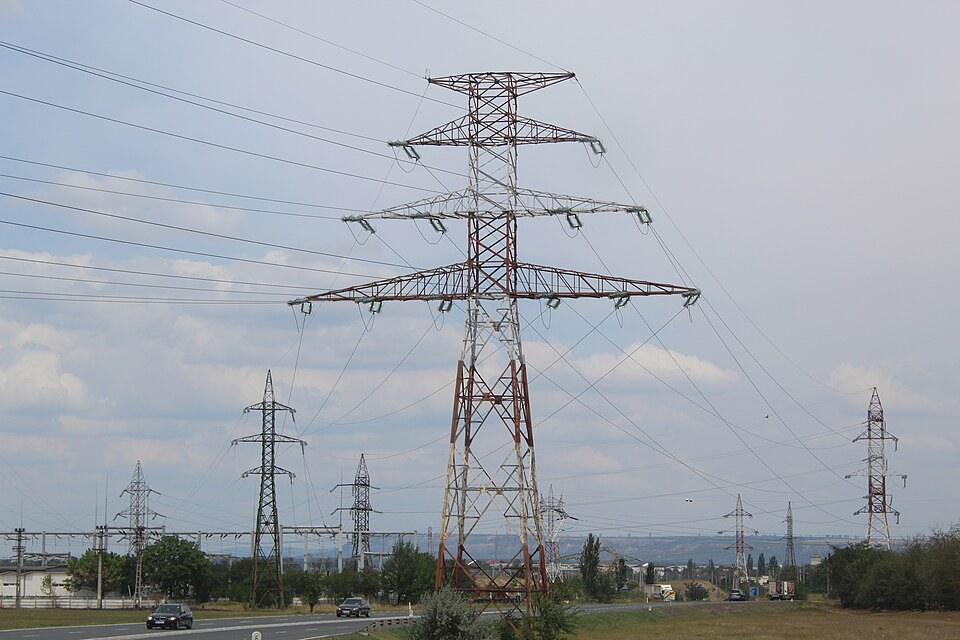
\includegraphics[height=0.45\textheight]{ch9_marasesti_750kv_2022.jpg}\\[1mm]
\imgcap{750 kV line at Mărășești: the Romanian transmission grid}
\imgcredit{https://commons.wikimedia.org/wiki/File:750_kV_electricity_tower_at_M\%C4\%83r\%C4\%83\%C8\%99e\%C8\%99ti,_Romania.jpg}{Photo: TrainSimFan (2022); CC BY-SA 4.0; Wikimedia Commons}
\end{column}
\begin{column}{0.64\textwidth}
\begin{itemize}
    \item The evaluation design of \tsachlink{https://danpele.github.io/Time-Series-Analysis/EN/Courses/chapter4_seasonality_forecasting.pdf}{Chapter 4}: 26 forecast origins every 14 days, 30 June 2025 to 15 June 2026
    \begin{itemize}
        \item horizon 1--14 days; expanding window from 1 January 2022
        \item statistical models (\tsachlink{https://danpele.github.io/Time-Series-Analysis/EN/Courses/chapter4_seasonality_forecasting.pdf}{Chapter 4}): seasonal naive, ETS, SARIMA, DHR (dynamic harmonic regression), their combination
    \end{itemize}
    \item ML models, refitted at each origin:
    \begin{itemize}
        \item direct: ridge, random forest (200 trees), GB (300 trees, $\nu = 0.05$), one model per horizon
        \item recursive: GB on the one-step table; MIMO: an MLP (3 networks, 32 neurons) and an LSTM (56 days in, 14 out)
    \end{itemize}
    \item MASE scale: in-sample MAE of the weekly seasonal naive method, 309 MW
\end{itemize}
\end{column}
\end{columns}
\end{frame}

\begin{frame}{Results: 26 origins, 14 horizons}
\itemsize{\footnotesize}
\begin{center}
\scriptsize
\begin{tabular}{lrrrr}
\toprule
\textbf{Model} & MAE (GW) & RMSE (GW) & MASE & DM p, against DHR \\
\midrule
Seasonal naive & 0.396 & 0.529 & 1.28 & $<$\,0.001 \\
ETS & 0.381 & 0.492 & 1.23 & 0.015 \\
SARIMA & 0.384 & 0.477 & 1.24 & 0.003 \\
DHR & 0.276 & 0.350 & 0.89 & -- \\
Combination & 0.305 & 0.380 & 0.99 & 0.065 \\
Ridge & 0.277 & 0.337 & 0.90 & 0.942 \\
RF & 0.308 & 0.388 & 1.00 & 0.068 \\
GB direct & 0.298 & 0.369 & 0.97 & 0.163 \\
GB recursive & 0.307 & 0.388 & 0.99 & 0.113 \\
MLP & 0.294 & 0.362 & 0.95 & 0.546 \\
LSTM & 0.357 & 0.447 & 1.16 & 0.016 \\
\bottomrule
\end{tabular}
\end{center}
\begin{itemize}
    \item DM: Diebold--Mariano test on the origin-average absolute errors (26 values), with the Harvey--Leybourne--Newbold correction \refHLN
\end{itemize}
\end{frame}

\begin{frame}{MASE and accuracy by horizon}
\itemsize{\footnotesize}
\begin{center}
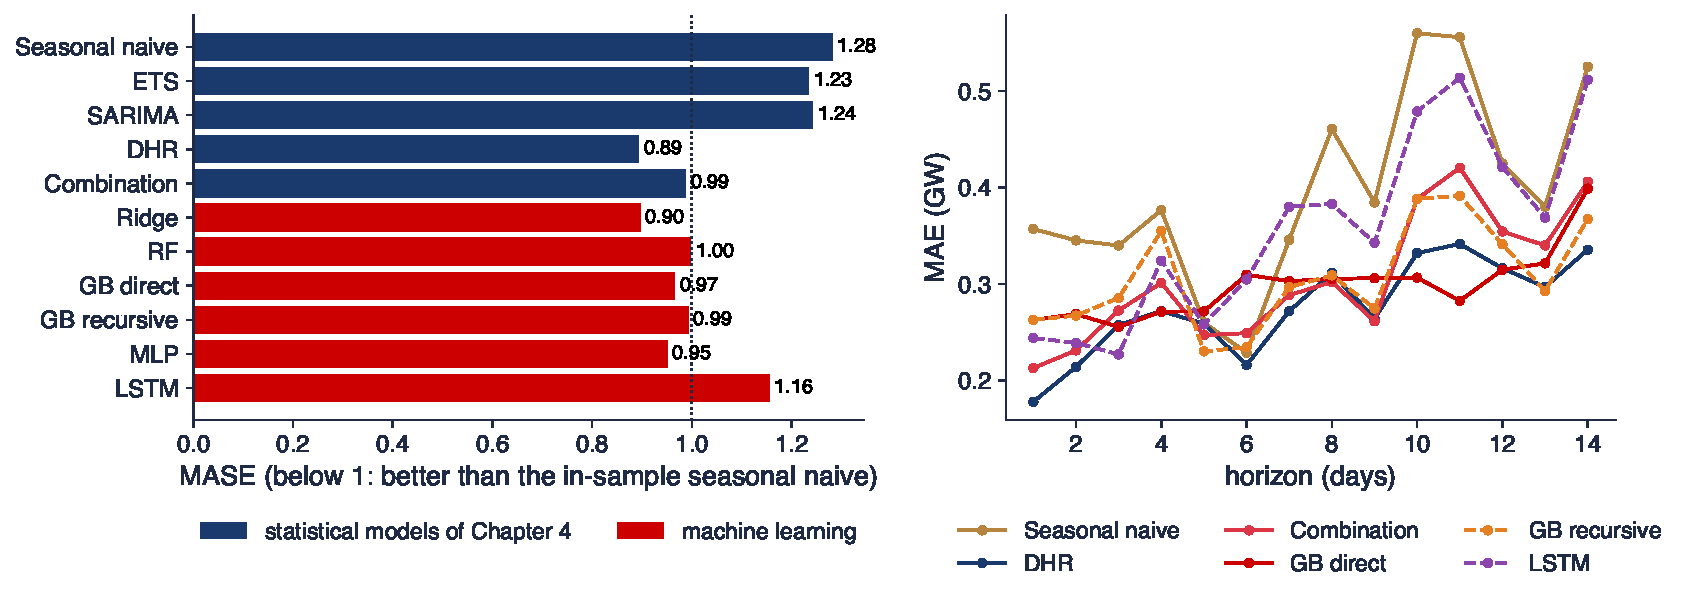
\includegraphics[width=0.97\textwidth,height=0.5\textheight,keepaspectratio]{tsa_ch9_load_results.pdf}
\end{center}
\vspace{-0.25cm}
\begin{itemize}
    \item Left: MASE of the eleven models (blue: \tsachlink{https://danpele.github.io/Time-Series-Analysis/EN/Courses/chapter4_seasonality_forecasting.pdf}{Chapter 4}; red: ML); right: MAE by horizon for six models
\end{itemize}
\quantlet{TSA\_ch9\_load\_forecasting}{\qlurl{TSA_ch9_load_forecasting}}
\end{frame}

\begin{frame}{Interpreting the load results}
\itemsize{\small}
\begin{itemize}
    \item DHR (MASE 0.89) and ridge (0.90) are the most accurate; the difference is not significant (p = 0.942)
    \begin{itemize}
        \item both are linear models with the right calendar features; the trees and networks do not beat them
    \end{itemize}
    \item GB direct (0.97), MLP (0.95), random forest (1.00) beat the seasonal naive method clearly (p = 0.001) and SARIMA, ETS
    \begin{itemize}
        \item direct and recursive GB are close (0.97 and 0.99); the LSTM (1.16) is worse than every model except the naive, SARIMA and ETS
    \end{itemize}
    \item Lesson: features matter more than the algorithm; with four years of daily data, a well-specified linear model is hard to beat
\end{itemize}
\end{frame}

\begin{frame}{Forecasts around Orthodox Easter 2026}
\itemsize{\footnotesize}
\begin{center}
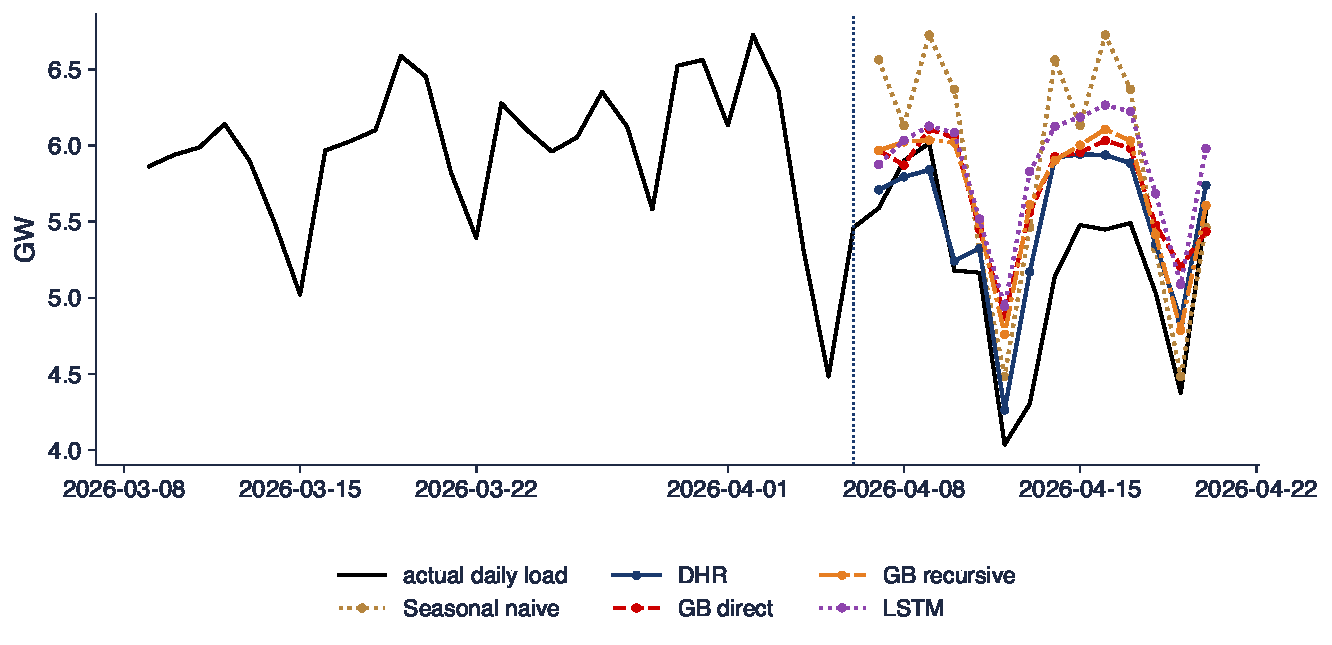
\includegraphics[width=0.97\textwidth,height=0.5\textheight,keepaspectratio]{tsa_ch9_load_forecasts.pdf}
\end{center}
\vspace{-0.25cm}
\begin{itemize}
    \item Origin 6 April 2026; 14-day forecasts; MAE in this window: DHR 344 MW, GB direct 536 MW, GB recursive 503 MW, LSTM 661 MW
\end{itemize}
\quantlet{TSA\_ch9\_load\_forecasting}{\qlurl{TSA_ch9_load_forecasting}}
\end{frame}

\begin{frame}{Interpreting the Easter window}
\itemsize{\small}
\begin{itemize}
    \item All models see the Easter flag, but the trees have only four Easters in training: they predict a dip that is too shallow
    \begin{itemize}
        \item DHR estimates one Easter coefficient from the same four episodes and pools the information more efficiently
    \end{itemize}
    \item The LSTM sees no holiday flag: it repeats the weekly pattern and misses the holiday entirely
    \item Rare events need either structure (a regression coefficient) or many series that share the event (a global model)
\end{itemize}
\end{frame}

\begin{frame}{Recap: Electricity load}
\itemsize{\small}
\begin{itemize}
    \item Same origins, same horizon, same errors: ML models enter the comparison of \tsachlink{https://danpele.github.io/Time-Series-Analysis/EN/Courses/chapter4_seasonality_forecasting.pdf}{Chapter 4}
    \item Ridge equals DHR; GB, random forest and the MLP beat SARIMA and ETS; the LSTM does not
    \item Calendar features and holidays decide the ranking
\end{itemize}
\end{frame}


%=============================================================================
\section{Prediction intervals}
%=============================================================================

\begin{frame}{Quantile regression and the pinball loss}
\itemsize{\footnotesize}
\begin{itemize}
    \item A point forecast is not enough: a grid operator needs the load it will not exceed with 95\% probability
    \begin{itemize}
        \item the $\tau$-quantile $q_\tau$ of $y_{t+h}$: $P(y_{t+h} \le q_\tau) = \tau$; a 90\% interval: $[q_{0.05}, q_{0.95}]$
    \end{itemize}
    \item \textbf{Pinball loss}: $L_\tau(y, q) = \tau(y - q)$ if $y \ge q$, and $(1 - \tau)(q - y)$ if $y < q$ \refKB
    \begin{itemize}
        \item its expected value is minimised by the true quantile; with $\tau = 0.5$ it is half the absolute error
        \item example, $\tau = 0.95$, $q = 7.0$ GW: $y = 7.4$ costs $0.95 \cdot 0.4 = 0.380$; $y = 6.5$ costs $0.05 \cdot 0.5 = 0.025$
    \end{itemize}
    \item Any learner can minimise the pinball loss: linear quantile regression, quantile GB (\texttt{loss='quantile'}), networks
\end{itemize}
\end{frame}

\begin{frame}{Split conformal prediction}
\itemsize{\footnotesize}
\begin{itemize}
    \item \textbf{Idea} \refLei: use the errors of the model on data it has not seen to set the width of the interval
    \begin{itemize}
        \item 1. fit the model on the training data except the last $n$ points (the calibration set)
        \item 2. compute the absolute errors $|e_i|$ on the calibration set and sort them
        \item 3. $\hat q$ = the $\lceil (n+1)(1 - \alpha) \rceil$-th smallest; interval $\hat y \pm \hat q$
        \item $\alpha$: the target miscoverage ($\alpha = 0.1$ for a 90\% interval); $\lceil\cdot\rceil$: rounding up
    \end{itemize}
    \item Guarantee: coverage at least $1 - \alpha$ if the errors are exchangeable (their order does not matter)
    \begin{itemize}
        \item time series are not exchangeable: the guarantee is approximate; use recent calibration data and recheck the coverage walk-forward
    \end{itemize}
    \item Here: $n = 182$ days, $\alpha = 0.1$, $\hat q$ = the 165-th smallest absolute error, one calibration set per horizon and origin
\end{itemize}
\end{frame}

\begin{frame}{90\% intervals for the load}
\itemsize{\footnotesize}
\begin{center}
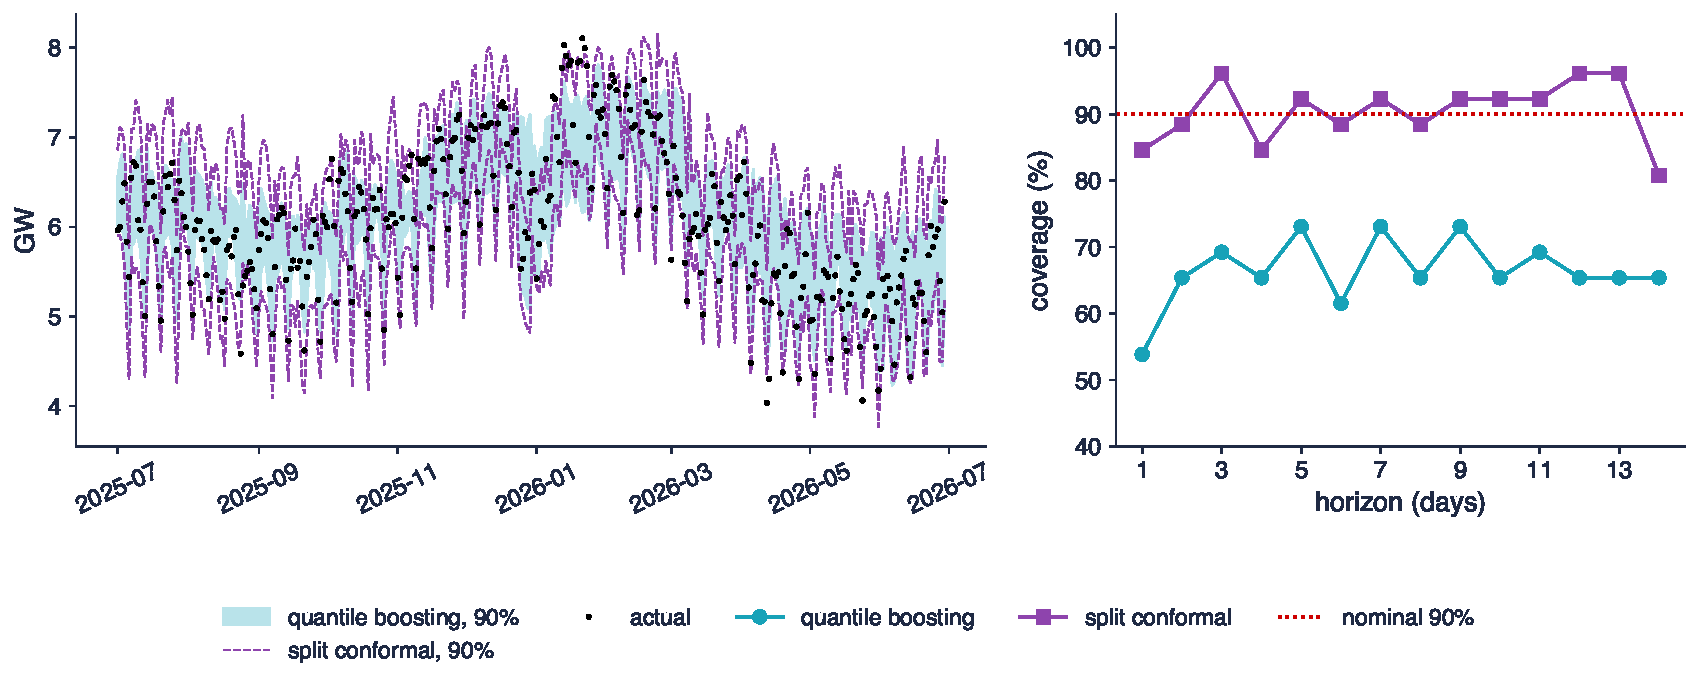
\includegraphics[width=0.97\textwidth,height=0.5\textheight,keepaspectratio]{tsa_ch9_intervals.pdf}
\end{center}
\vspace{-0.25cm}
\begin{itemize}
    \item Direct GB, the 364 forecasts of Section 6 (all origins and horizons); left: intervals and outcomes; right: coverage by horizon
\end{itemize}
\quantlet{TSA\_ch9\_load\_forecasting}{\qlurl{TSA_ch9_load_forecasting}}
\end{frame}

\begin{frame}{Interpreting the intervals}
\itemsize{\small}
\begin{itemize}
    \item Quantile GB covers 66.5\% with mean width 884 MW; split conformal covers 90.4\% with width 1310 MW
    \begin{itemize}
        \item quantile GB: 19.0\% of outcomes below and 14.6\% above the interval (nominal 5\% and 5\%)
    \end{itemize}
    \item Quantiles estimated by trees are noisy in the tails and too narrow; conformal calibration corrects the width with real out-of-sample errors
    \item Always report the empirical coverage next to an interval
\end{itemize}
\end{frame}

\begin{frame}{Recap: Prediction intervals}
\itemsize{\small}
\begin{itemize}
    \item Quantile forecasts minimise the pinball loss; an interval is a pair of quantiles
    \item Split conformal: $\hat y \pm$ an empirical quantile of calibration errors
    \item Check the coverage walk-forward
\end{itemize}
\end{frame}


%=============================================================================
\section{Local and global models: Romanian inflation}
%=============================================================================

\begin{frame}{Local and global models}
\itemsize{\small}
\begin{itemize}
    \item \textbf{Local} model: one model per series, estimated on that series only (ARIMA, ETS, the models so far)
    \begin{itemize}
        \item few observations per series limit the complexity a local model can afford
    \end{itemize}
    \item \textbf{Global} model: one model estimated on the pooled rows of many related series \refMMH, \refJanus
    \begin{itemize}
        \item the same features for every series (scaled lags, calendar); optionally a series identifier
        \item more data per parameter: complex learners (GB, networks) become usable; the winners of M4 and M5 were global
    \end{itemize}
    \item Risk: the series must share dynamics; a global model may average away what is special about one series
\end{itemize}
\end{frame}

\begin{frame}{The inflation exercise}
\itemsize{\footnotesize}
\begin{itemize}
    \item Target: 12-month HICP inflation of Romania (Eurostat), $\pi_t = 100(P_t/P_{t-12} - 1)$, $P_t$: the HICP index, at horizons $h = 1, 3, 6, 12$ months
    \begin{itemize}
        \item direct strategy; the models forecast the change $\pi_{t+h} - \pi_t$, so trees never extrapolate the level
    \end{itemize}
    \item Features at $t$: $\pi_t, \pi_{t-1}, \pi_{t-2}, \pi_{t-3}, \pi_{t-6}, \pi_{t-12}$, the last three monthly log changes and their 3- and 6-month sums, the calendar month
    \begin{itemize}
        \item models: random walk (RW, $\hat\pi_{t+h} = \pi_t$), AR (OLS on the same features), lasso, random forest, GB local (Romania only), GB global (27 EU countries pooled)
    \end{itemize}
    \item Walk-forward: refit every January on all rows whose target month is already observed (from 2006); test origins January 2016--July 2026
    \item Related evidence: \refMedeiros\ find that random forests beat the benchmarks for US inflation with more than 100 predictors
\end{itemize}
\end{frame}

\begin{frame}{Romanian inflation: forecasts and relative RMSE}
\itemsize{\footnotesize}
\begin{center}
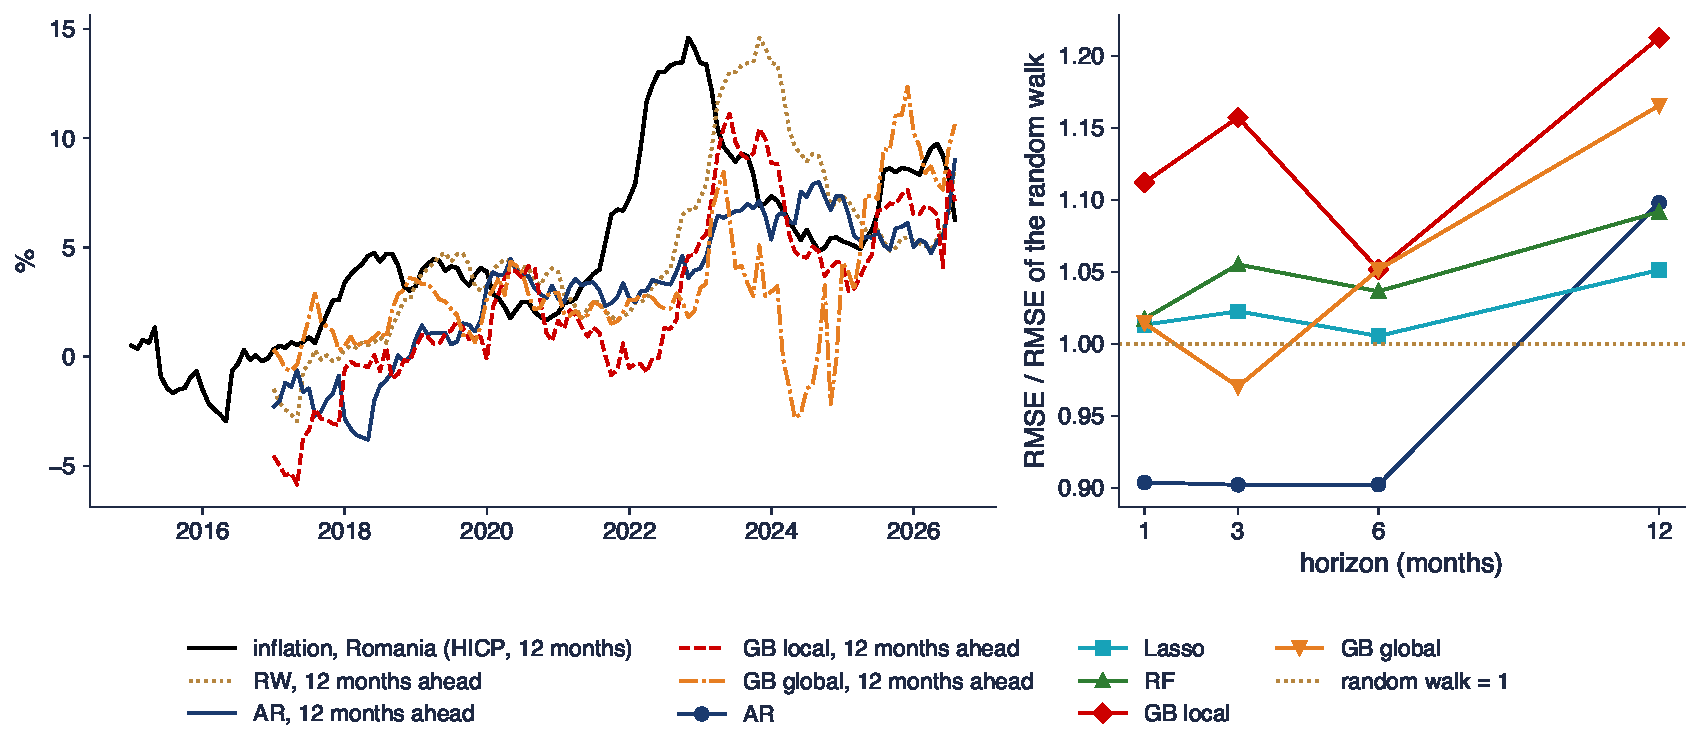
\includegraphics[width=0.97\textwidth,height=0.52\textheight,keepaspectratio]{tsa_ch9_inflation.pdf}
\end{center}
\vspace{-0.25cm}
\begin{itemize}
    \item Left: inflation and the 12-month-ahead forecasts plotted at the target month; right: RMSE relative to the random walk
\end{itemize}
\quantlet{TSA\_ch9\_inflation\_global}{\qlurl{TSA_ch9_inflation_global}}
\end{frame}

\begin{frame}{Inflation results}
\itemsize{\footnotesize}
\begin{center}
\scriptsize
\begin{tabular}{lrrrr}
\toprule
\textbf{RMSE (pp), relative to RW} & $h = 1$ & $h = 3$ & $h = 6$ & $h = 12$ \\
\midrule
RW & 0.63 (1.00) & 1.41 (1.00) & 2.25 (1.00) & 3.90 (1.00) \\
AR & 0.57 (0.90) & 1.28 (0.90) & 2.03 (0.90) & 4.28 (1.10) \\
Lasso & 0.64 (1.01) & 1.45 (1.02) & 2.26 (1.01) & 4.10 (1.05) \\
RF & 0.64 (1.02) & 1.49 (1.06) & 2.33 (1.04) & 4.25 (1.09) \\
GB local & 0.70 (1.11) & 1.64 (1.16) & 2.37 (1.05) & 4.72 (1.21) \\
GB global & 0.64 (1.01) & 1.37 (0.97) & 2.37 (1.05) & 4.54 (1.17) \\
\bottomrule
\end{tabular}
\end{center}
\begin{itemize}
    \item DM p against RW, AR: 0.019 ($h = 1$), 0.186 ($h = 3$), 0.388 ($h = 6$); GB global against GB local: 0.117, 0.113, 0.999, 0.828
    \item Test origins: 127 ($h = 1$) to 116 ($h = 12$) months; DM with squared errors and $h - 1$ autocovariances
\end{itemize}
\end{frame}

\begin{frame}{Interpreting the inflation results}
\itemsize{\small}
\begin{itemize}
    \item The linear AR is the best model up to 6 months (about 10\% below the random walk); no ML model beats the random walk significantly
    \begin{itemize}
        \item at 12 months nothing beats the random walk: the 2022 peak (14.6\% in November 2022) came from energy prices, not from the past of inflation
    \end{itemize}
    \item The global GB is better than the local one at short horizons (RMSE 1.37 against 1.64 at $h = 3$), but not significantly (p = 0.113)
    \begin{itemize}
        \item pooling 27 countries gives the trees enough rows; the local GB, with 120--240 rows per refit, overfits
    \end{itemize}
    \item About 120 monthly test errors cannot separate models whose RMSEs differ by 5\%: the honest conclusion is ``no evidence''
\end{itemize}
\end{frame}

\begin{frame}{Recap: Local and global models}
\itemsize{\small}
\begin{itemize}
    \item A global model pools many related series and lets flexible learners use more data
    \item Romanian inflation: AR is best; global GB beats local GB; nothing beats the random walk at 12 months
    \item Small samples: report DM p-values, not only RMSE rankings
\end{itemize}
\end{frame}


%=============================================================================
\section{Applications in finance: volatility and the sign of returns}
%=============================================================================

\begin{frame}{Realised volatility: HAR against ML (1/2)}
\itemsize{\footnotesize}
\begin{itemize}
    \item Target: the log of the mean daily variance over the next 5 days; daily variance proxy from open, high, low and close prices \refGK
    \begin{itemize}
        \item $\hat\sigma_t^2 = [\ln(O_t/C_{t-1})]^2 + \frac12[\ln(H_t/L_t)]^2 - (2\ln 2 - 1)[\ln(C_t/O_t)]^2$: the overnight return squared plus the Garman--Klass term
        \item $O_t$, $H_t$, $L_t$, $C_t$: the open, high, low and close of day $t$
        \item volatility is persistent and predictable (\tsachlink{https://danpele.github.io/Time-Series-Analysis/EN/Courses/chapter5_conditional_volatility_garch.pdf}{Chapter 5}): the right ground for ML
    \end{itemize}
    \item \textbf{HAR} (heterogeneous autoregressive) model \refCorsi: OLS on the log variance of the last day, week and month
    \begin{itemize}
        \item $\ln \bar\sigma^2_{t+1:t+5} = c + \beta_d \ln\hat\sigma_t^2 + \beta_w \ln\bar\sigma^2_{t-4:t} + \beta_m \ln\bar\sigma^2_{t-21:t} + u_t$; $\bar\sigma^2_{a:b}$: the mean of $\hat\sigma^2$ over days $a$ to $b$; $u_t$: the error
        \item ML models add 8 features: lags of the daily variance, the quarterly mean, the return, its negative part and its absolute value
    \end{itemize}
\end{itemize}
\end{frame}

\begin{frame}{Realised volatility: HAR against ML (2/2)}
\itemsize{\footnotesize}
\begin{itemize}
    \item Yearly walk-forward from 2013 with a 5-day gap between training and test
    \item Out-of-sample $R^2$ against HAR: $R^2_{\text{HAR}} = 1 - \sum_t (y_t - \hat y_t)^2 / \sum_t (y_t - \hat y_t^{\text{HAR}})^2$
    \begin{itemize}
        \item $y_t$: the realised log variance; $\hat y_t$, $\hat y_t^{\text{HAR}}$: the forecasts of the model and of HAR; positive: better than HAR
    \end{itemize}
    \item QLIKE \refPatton: $L(\sigma^2, h) = \sigma^2/h + \ln h$, the quasi-likelihood loss for variances (\tsachlink{https://danpele.github.io/Time-Series-Analysis/EN/Courses/chapter5_conditional_volatility_garch.pdf}{Chapter 5}); lower is better
    \begin{itemize}
        \item $\sigma^2$: the realised variance; $h$: the variance forecast; for a given $\sigma^2$ the loss is smallest at $h = \sigma^2$ and penalises forecasts that are too low more
        \item robust to the noise of the variance proxy: it ranks forecasts as the true variance would
    \end{itemize}
    \item Diebold--Mariano test (\tsachlink{https://danpele.github.io/Time-Series-Analysis/EN/Courses/chapter4_seasonality_forecasting.pdf}{Chapter 4}) on the daily QLIKE differences
\end{itemize}
\end{frame}

\begin{frame}{Results: S\&P 500 and DAX, 2013--2026}
\itemsize{\footnotesize}
\begin{center}
\scriptsize
\begin{tabular}{lrrrrrr}
\toprule
\textbf{Model} & S\&P: $R^2$ vs HAR (\%) & QLIKE & DM $t$ & DAX: $R^2$ vs HAR (\%) & QLIKE & DM $t$ \\
\midrule
HAR & +0.0 & 0.414 & -- & +0.0 & 1.023 & -- \\
Lasso & +7.1 & 0.400 & $-$5.12 & +7.9 & 1.015 & $-$2.42 \\
RF & +1.0 & 0.416 & 0.32 & +3.5 & 1.024 & 0.03 \\
GB & $-$0.5 & 0.416 & 0.35 & +1.1 & 1.028 & 0.75 \\
MLP & +8.3 & 0.398 & $-$3.96 & +8.6 & 1.015 & $-$1.69 \\
\bottomrule
\end{tabular}
\end{center}
\begin{itemize}
    \item 3\,444 and 3\,473 test days; DM $t < -1.96$: the model has a significantly lower QLIKE than HAR
    \item The lasso and the MLP gain 7--9\% of $R^2$ over HAR and lower QLIKE significantly on the S\&P 500; the random forest and GB do not beat HAR
    \item The gain comes from the extra features (the negative return: the leverage effect of \tsachlink{https://danpele.github.io/Time-Series-Analysis/EN/Courses/chapter5_conditional_volatility_garch.pdf}{Chapter 5}), used smoothly; trees cut a smooth relation into steps
\end{itemize}
\end{frame}

\begin{frame}{Volatility forecasts in two storms}
\itemsize{\footnotesize}
\begin{center}
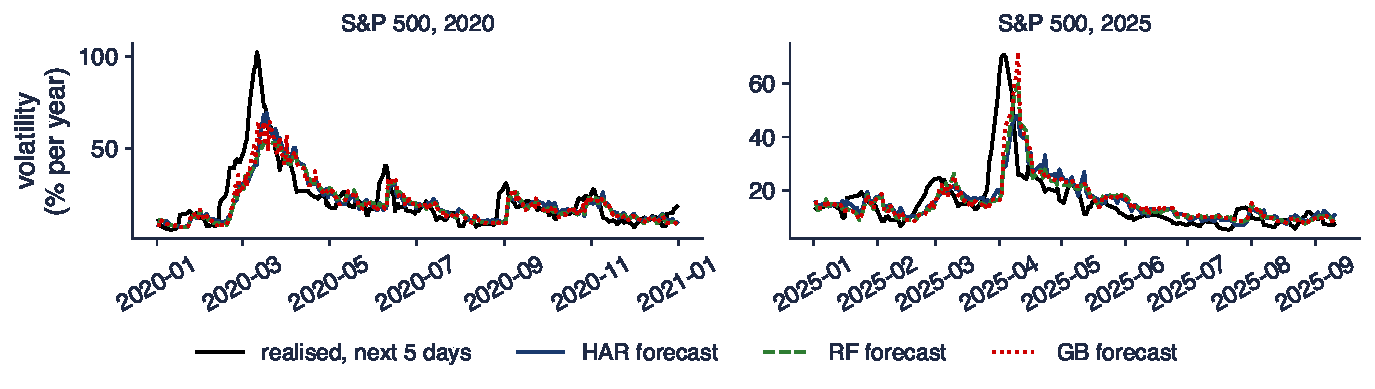
\includegraphics[width=0.97\textwidth,height=0.52\textheight,keepaspectratio]{tsa_ch9_rv.pdf}
\end{center}
\vspace{-0.25cm}
\begin{itemize}
    \item S\&P 500: annualised realised volatility of the next 5 days and the HAR, random forest and GB forecasts, 2020 and 2025
\end{itemize}
\quantlet{TSA\_ch9\_finance}{\qlurl{TSA_ch9_finance}}
\end{frame}

\begin{frame}{The sign of tomorrow's return: the right baseline}
\itemsize{\footnotesize}
\begin{itemize}
    \item Classification: target $1\{r_{t+1} > 0\}$ (1 if tomorrow's return is positive, 0 otherwise); features: the last five returns, sums over 5, 21, 63 days, volatility over 21 and 63 days
    \begin{itemize}
        \item models: logistic regression (logit), random forest, GB; yearly walk-forward from 2008
    \end{itemize}
    \item \textbf{The right baseline} is not 50\%: markets rise on more days than they fall
    \begin{itemize}
        \item ``always up'' (the majority class of the training data) is right on 54.4\% of S\&P 500 days and 53.8\% of BET days
    \end{itemize}
    \item Accuracy, S\&P 500: logit 53.8\%, random forest 53.1\%, GB 52.5\%; BET: 53.7\%, 53.6\%, 52.2\%
    \item No model beats the baseline; AUC (area under the ROC curve) 0.511--0.533, close to 0.5: no ranking skill either
    \begin{itemize}
        \item AUC: the probability that a randomly chosen up day gets a higher model score than a randomly chosen down day; 0.5: no skill, 1: perfect ranking
    \end{itemize}
\end{itemize}
\end{frame}

\begin{frame}{Accuracy against the baseline}
\itemsize{\footnotesize}
\begin{center}
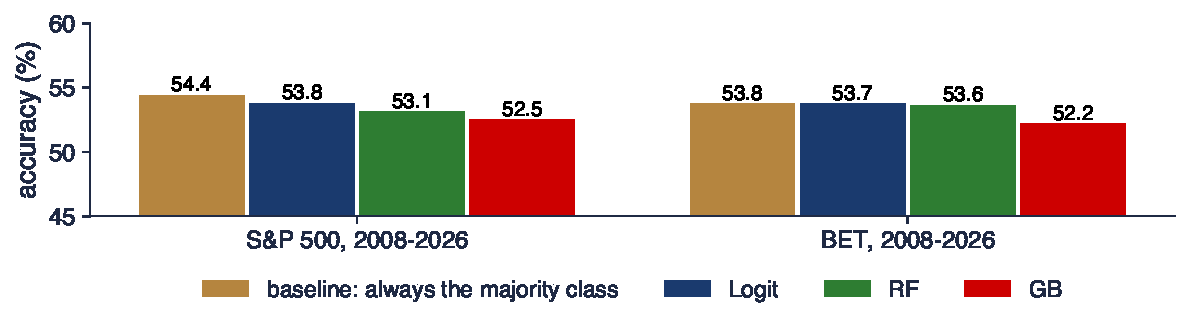
\includegraphics[width=0.97\textwidth,height=0.48\textheight,keepaspectratio]{tsa_ch9_sign.pdf}
\end{center}
\vspace{-0.25cm}
\begin{itemize}
    \item Out-of-sample accuracy 2008--2026: 4\,705 S\&P 500 days and 4\,686 BET days
\end{itemize}
\quantlet{TSA\_ch9\_finance}{\qlurl{TSA_ch9_finance}}
\end{frame}

\begin{frame}{Interpreting the sign experiment}
\itemsize{\small}
\begin{itemize}
    \item A model with ``53\% accuracy'' sounds skilful; against the 54.4\% of ``always up'' it is worse than doing nothing
    \begin{itemize}
        \item GB on the S\&P 500 is significantly worse than the baseline (p = 0.008): flexible models fit noise
    \end{itemize}
    \item Weak-form efficiency (\tsachlink{https://danpele.github.io/Time-Series-Analysis/EN/Courses/chapter1_stochastic_processes_stationarity.pdf}{Chapter 1}): past returns contain almost no information about the sign of the next one
    \item Volatility is predictable, the direction is not: ML confirms what the statistical models of \tsachlink{https://danpele.github.io/Time-Series-Analysis/EN/Courses/chapter1_stochastic_processes_stationarity.pdf}{Chapters 1} and \tsachlink{https://danpele.github.io/Time-Series-Analysis/EN/Courses/chapter5_conditional_volatility_garch.pdf}{5} showed
\end{itemize}
\end{frame}

\begin{frame}{Recap: Volatility and the sign of returns}
\itemsize{\small}
\begin{itemize}
    \item Realised volatility: lasso and MLP with extra features beat HAR; trees do not
    \item Sign of returns: compare with the majority class, not with 50\%; no model beats it
\end{itemize}
\end{frame}


%=============================================================================
\section{Landmark case studies: M4, M5 and Gu, Kelly and Xiu}
%=============================================================================

\begin{frame}{The M competitions}
\itemsize{\footnotesize}
\begin{itemize}
    \item Since 1982 Spyros Makridakis has organised open forecasting competitions: all methods forecast the same series, evaluated by the organisers on hidden data
    \begin{itemize}
        \item the honest version of the walk-forward test: no participant can tune on the test data
    \end{itemize}
    \item \refMSAplos: on 1\,045 monthly series of M3, popular ML methods were less accurate than eight statistical methods at every horizon, and much slower
    \item M4 (2018), \refMfour: 100\,000 series of six frequencies, 61 methods, ranked by OWA (overall weighted average)
    \begin{itemize}
        \item $\text{OWA} = \frac12\bigl(\text{sMAPE}/\text{sMAPE}_{N2} + \text{MASE}/\text{MASE}_{N2}\bigr)$; $N2$: Naive2, the naive forecast of the seasonally adjusted series; below 1: better than Naive2
        \item sMAPE (symmetric mean absolute percentage error) $= \frac{200}{H}\sum_{h=1}^{H} |y_{T+h} - \hat y_{T+h}| / (|y_{T+h}| + |\hat y_{T+h}|)$, in \%
    \end{itemize}
    \item M5 (2020), \refMfive: 42\,840 hierarchical daily series of Walmart unit sales, 28-day horizon
\end{itemize}
\end{frame}

\begin{frame}{M4: the accuracy of all methods}
\itemsize{\footnotesize}
\begin{center}
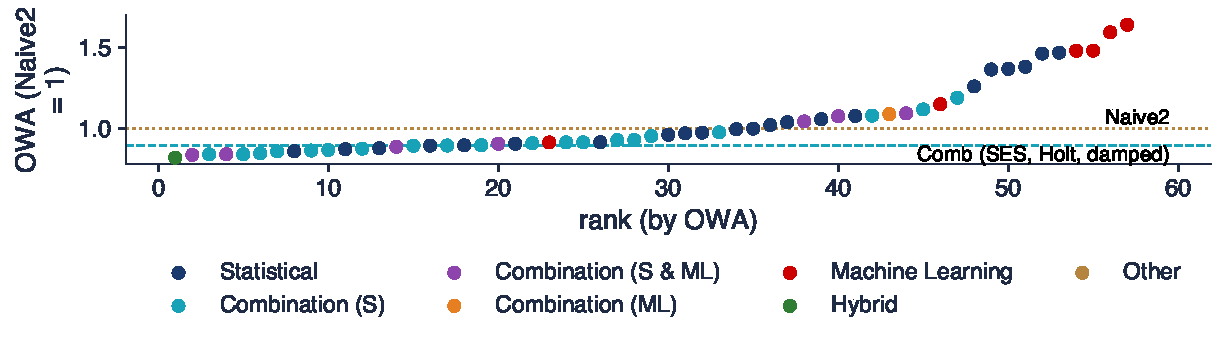
\includegraphics[width=0.97\textwidth,height=0.5\textheight,keepaspectratio]{tsa_ch9_m4.pdf}
\end{center}
\vspace{-0.25cm}
\begin{itemize}
    \item Official evaluation file of M4 (github.com/Mcompetitions/M4-methods): OWA of the 59 ranked methods, submissions and benchmarks, coloured by type; 2 methods with OWA above 1.7 are off the chart
\end{itemize}
\quantlet{TSA\_ch9\_case\_studies}{\qlurl{TSA_ch9_case_studies}}
\end{frame}

\begin{frame}{Interpreting M4}
\itemsize{\small}
\begin{itemize}
    \item Winner: the hybrid ES-RNN of \refSmyl, exponential smoothing inside an LSTM trained on all series (a global model): OWA 0.821, sMAPE 11.37\%
    \begin{itemize}
        \item Comb, the average of SES, Holt and damped trend: OWA 0.898, sMAPE 12.55\%; Naive2: sMAPE 13.56\%
    \end{itemize}
    \item The 6 pure ML methods: the best ranked 23 (OWA 0.915); none beat Comb, only one beat Naive2 \refMfourA
    \begin{itemize}
        \item 12 of the 17 best methods were combinations
    \end{itemize}
    \item Lesson: on short, heterogeneous series, combine statistical models, or let ML learn across series; pure local ML loses
\end{itemize}
\end{frame}

\begin{frame}{M5: gradient boosting wins on retail data}
\itemsize{\footnotesize}
\begin{columns}[T]
\begin{column}{0.36\textwidth}
\centering

\includegraphics[height=0.42\textheight]{ch9_walmart_store.jpg}\\[1mm]
\imgcap{A Walmart store: the M5 data are the daily unit sales of 3\,049 products in 10 stores}
\imgcredit{https://commons.wikimedia.org/wiki/File:Walmart_store_exterior_5266815680.jpg}{Photo: Walmart Corporate; CC BY 2.0; Wikimedia Commons}
\end{column}
\begin{column}{0.62\textwidth}
\begin{itemize}
    \item 5\,507 teams from 101 countries; error measure WRMSSE (weighted root mean squared scaled error)
    \begin{itemize}
        \item RMSSE: the RMSE of the forecasts over the in-sample RMSE of the one-step naive forecast
        \item WRMSSE: the average RMSSE, weighted by sales value
        \item the winner (WRMSSE 0.520) was 22.4\% more accurate than the best benchmark, bottom-up exponential smoothing (0.671)
    \end{itemize}
    \item Most top methods used LightGBM \refLGBM
    \begin{itemize}
        \item the winner averaged LightGBM models pooled by store, category and department, recursive and direct
        \item global models, rich calendar and price features, many related series: the conditions where ML wins
    \end{itemize}
\end{itemize}
\end{column}
\end{columns}
\end{frame}

\begin{frame}{Gu, Kelly and Xiu (2020): machine learning for stock returns}
\itemsize{\footnotesize}
\begin{columns}[T]
\begin{column}{0.34\textwidth}
\centering
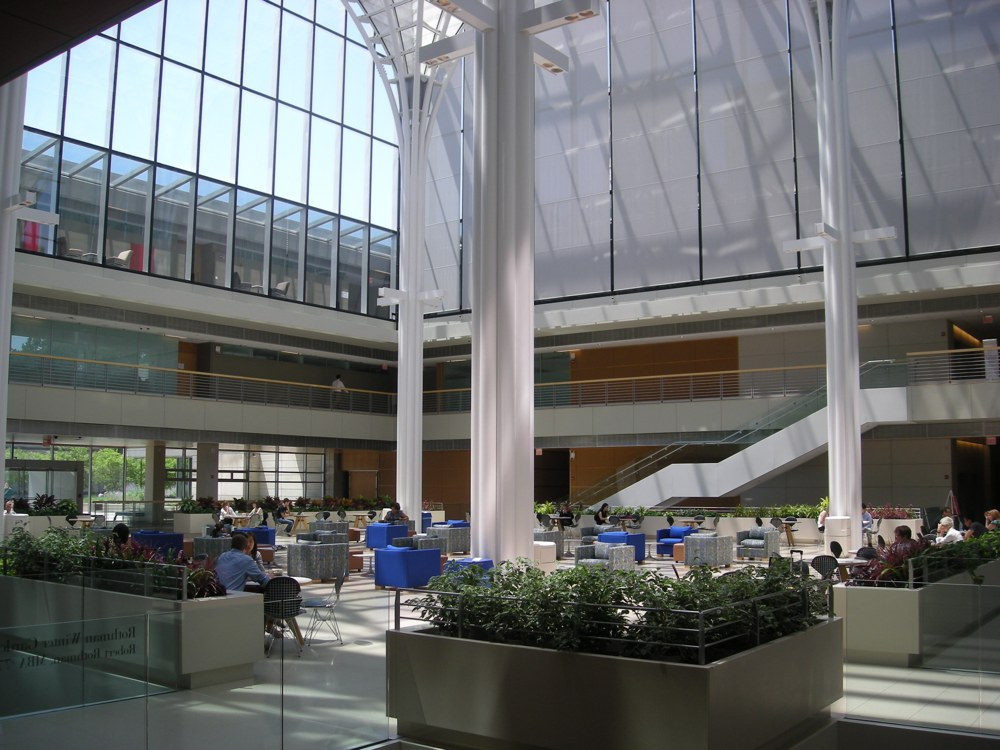
\includegraphics[height=0.36\textheight]{ch9_harper_center_2013.jpg}\\[1mm]
\imgcap{Charles M. Harper Center, University of Chicago Booth School of Business}
\imgcredit{https://commons.wikimedia.org/wiki/File:University_of_Chicago_July_2013_01_(Charles_M._Harper_Center).jpg}{Photo: Michael Barera (2013); CC BY-SA 4.0; Wikimedia Commons}
\end{column}
\begin{column}{0.64\textwidth}
\begin{itemize}
    \item \refGKX: monthly returns of about 30\,000 US stocks, 1957--2016, 920 predictors
    \begin{itemize}
        \item 12 methods, from OLS to neural networks with five layers
        \item walk-forward: 18 years of training, 12 of validation, 30 years of test, refitted yearly
    \end{itemize}
    \item Out-of-sample monthly $R^2$: at most 0.40\% (three-layer network); OLS with all predictors: $-3.46$\%
    \item Small $R^2$, large value: a long-short portfolio sorted on the forecasts reaches an annual Sharpe ratio of 1.35 (four layers), against 0.61 for OLS-3
    \begin{itemize}
        \item long-short: buy the decile with the highest forecasts, sell the decile with the lowest
        \item Sharpe ratio: the mean annual return divided by its annual standard deviation
    \end{itemize}
\end{itemize}
\end{column}
\end{columns}
\end{frame}

\begin{frame}{Gu, Kelly and Xiu (2020): small $R^2$, large economic value}
\itemsize{\footnotesize}
\begin{center}
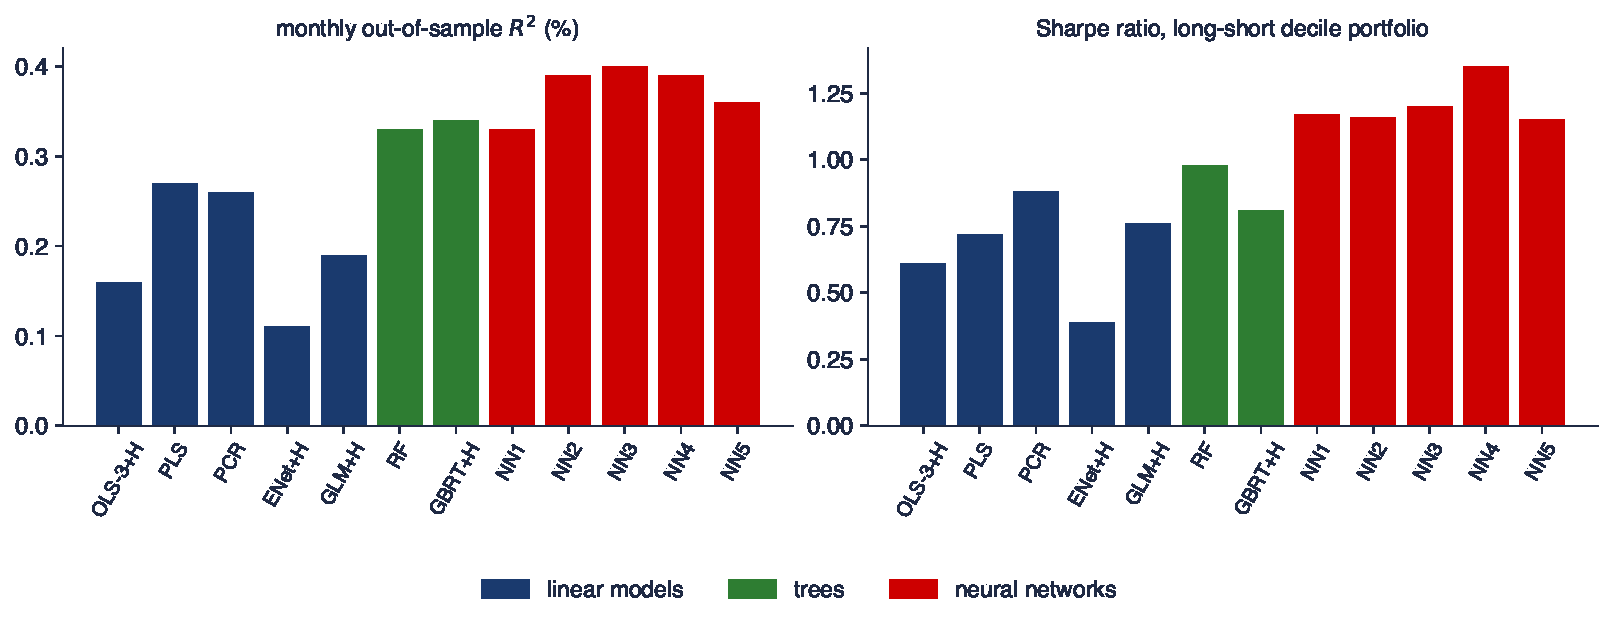
\includegraphics[width=0.97\textwidth,height=0.4\textheight,keepaspectratio]{tsa_ch9_gkx.pdf}
\end{center}
\vspace{-0.25cm}
\begin{itemize}
    \item Published numbers: Table 1 (monthly out-of-sample $R^2$, all stocks) and Table 7 (annualised Sharpe ratio of the value-weighted long-short decile portfolio); +H: Huber loss
    \item OLS-3: OLS on size, book-to-market and momentum; PLS, PCR: partial least squares, principal component regression; ENet: elastic net
    \item GLM: generalised linear model with splines; RF: random forest; GBRT: gradient-boosted regression trees; NN1--NN5: networks with 1--5 hidden layers
\end{itemize}
\quantlet{TSA\_ch9\_case\_studies}{\qlurl{TSA_ch9_case_studies}}
\end{frame}

\begin{frame}{Recap: Case studies}
\itemsize{\small}
\begin{itemize}
    \item M4: combinations and a hybrid global model win; pure local ML loses to simple benchmarks
    \item M5: global LightGBM models with calendar and price features win clearly
    \item Gu, Kelly and Xiu: tiny but real predictability in the cross-section of stocks; nonlinear models add value
\end{itemize}
\end{frame}


%=============================================================================
\section{Possible contribution of AI}
%=============================================================================

\begin{frame}{Foundation models: a pointer to \tsachlinkt{https://danpele.github.io/Time-Series-Analysis/EN/Courses/chapter11_foundation_models_time_series.pdf}{Chapter 11}}
\itemsize{\small}
\begin{itemize}
    \item A \textbf{foundation model} for time series is a large network (a transformer) pre-trained on millions of series and used without retraining (zero-shot)
    \begin{itemize}
        \item the extreme global model: Chronos, TimesFM, Moirai, Lag-Llama (self-study, \tsachlink{https://danpele.github.io/Time-Series-Analysis/EN/Courses/chapter11_foundation_models_time_series.pdf}{Chapter 11})
    \end{itemize}
    \item The same rules apply: walk-forward on data the model has not seen in pre-training, the same benchmarks, MASE and DM
\end{itemize}
\end{frame}

\begin{frame}{Possible contribution of AI}
\itemsize{\small}
\begin{itemize}
    \item \textbf{Code}: a first draft of the feature table, the walk-forward loop and the evaluation table
    \item \textbf{Explanation}: a second explanation of boosting, of the LSTM gates or of conformal prediction
    \item \textbf{Exploration}: many feature sets and hyperparameters at once (on validation data only)
    \item Example prompt
    \begin{itemize}
        \item \aiprompt{Write Python code that builds lag, rolling-mean and calendar features for daily electricity load, trains HistGradientBoostingRegressor with the direct strategy for horizons 1-14, evaluates it walk-forward against the seasonal naive forecast with MASE and the Diebold-Mariano test, and refits every preprocessing step inside each training window.}
    \end{itemize}
\end{itemize}
\end{frame}

\begin{frame}{Checks you must run}
\itemsize{\small}
\begin{itemize}
    \item Every feature uses data up to the origin only: check the shifts of lags and rolling windows on a printed table
    \item No \texttt{KFold(shuffle=True)}, no scaler or feature selection fitted on the full sample
    \item The benchmarks are there: naive or seasonal naive, ETS or ARIMA, on the same origins
    \item The comparison has a DM test; the classification has the majority-class baseline
    \item Seeds are fixed and the result survives another seed
    \item Every cited reference exists: check the DOI
\end{itemize}
\end{frame}


%=============================================================================
\section{Summary}
%=============================================================================

\begin{frame}{Key takeaways}
\itemsize{\small}
\begin{itemize}
    \item ML forecasting = supervised learning on a table of lags, rolling statistics and calendar features known at the origin
    \item Walk-forward validation only; leakage produces spectacular and false scores
    \item Ridge and lasso, random forest, GB, MLP, LSTM: each has a complexity knob set by validation
    \item Trees cannot extrapolate: model changes, not levels
    \item Our data: linear models with good features match or beat ML on load and inflation; ML helps for volatility; nothing predicts the sign of returns
    \item ML wins with many related series (global models, M4 hybrid, M5 LightGBM); always compare with benchmarks, MASE and DM
\end{itemize}
\end{frame}

\begin{frame}{Key formulas}
\itemsize{\small}
{\renewcommand{\arraystretch}{1.35}\begin{center}
\footnotesize
\begin{tabular}{ll}
\toprule
\textbf{Quantity} & \textbf{Formula} \\
\midrule
Direct forecast & $\hat y_{T+h} = \hat f_h(y_T, \dots, y_{T-p+1}, \mathbf{z}_{T+h})$, $\mathbf{z}_{T+h}$: calendar features \\
Ridge, lasso & $\min \sum_t (y_t - \mathbf{x}_t'\beta)^2 + \lambda\sum_j\beta_j^2$; \quad $+ \lambda\sum_j|\beta_j|$ \\
Bias--variance & $E[(y_0 - \hat f(x_0))^2] = \text{bias}^2 + \Var(\hat f(x_0)) + \sigma^2$ \\
Boosting & $F_m(\mathbf{x}) = F_{m-1}(\mathbf{x}) + \nu\,g_m(\mathbf{x})$ \\
MLP & $\hat y = c + \sum_j v_j\,g(b_j + \mathbf{w}_j'\mathbf{x})$ \\
LSTM & $c_t = f_t \odot c_{t-1} + i_t \odot \tilde c_t$, \quad $h_t = o_t \odot \tanh(c_t)$ \\
Pinball loss & $L_\tau(y, q) = \max(\tau(y - q), (\tau - 1)(y - q))$ \\
Split conformal & $\hat y \pm \hat q$, \quad $\hat q = |e|_{(\lceil (n+1)(1-\alpha) \rceil)}$ \\
MASE & $\text{MAE} / \frac{1}{n-m}\sum_{t>m}|y_t - y_{t-m}|$ \\
\bottomrule
\end{tabular}
\end{center}
}
\end{frame}

\begin{frame}{Self-assessment}
\itemsize{\small}
\begin{itemize}
    \item \textbf{Question}: a 7-day moving average centred on $t$ is used as a feature for $y_{t+1}$. Is that allowed?
    \begin{itemize}
        \item \textbf{Answer}: no: it contains $y_{t+1}, y_{t+2}, y_{t+3}$; use the trailing mean of $y_{t-6}, \dots, y_t$
    \end{itemize}
    \item \textbf{Question}: a random forest trained on GDP levels up to 2019 forecasts 2024. What goes wrong?
    \begin{itemize}
        \item \textbf{Answer}: its forecast cannot exceed the largest level seen in training; model growth rates
    \end{itemize}
    \item \textbf{Question}: a classifier predicts the sign of daily returns with 53\% accuracy. Is it useful?
    \begin{itemize}
        \item \textbf{Answer}: only if it beats the share of up days in the test period (about 54\% for the S\&P 500), significantly
    \end{itemize}
    \item Next: \tsachlink{https://danpele.github.io/Time-Series-Analysis/EN/Courses/chapter10_state_space_kalman_markov_switching.pdf}{Chapter 10}, state space models, the Kalman filter and Markov switching
\end{itemize}
\end{frame}


%=============================================================================
\section{References}
%=============================================================================

\begin{frame}{References (1/3)}
\itemsize{\tiny}
\begin{itemize}
    \item Ben Taieb, S., Bontempi, G., Atiya, A. F., \& Sorjamaa, A. (2012). A review and comparison of strategies for multi-step ahead time series forecasting based on the NN5 forecasting competition. \textit{Expert Systems with Applications}, 39(8), 7067--7083. \href{https://doi.org/10.1016/j.eswa.2012.01.039}{doi:10.1016/j.eswa.2012.01.039}
    \item Bergmeir, C., Hyndman, R. J., \& Koo, B. (2018). A note on the validity of cross-validation for evaluating autoregressive time series prediction. \textit{Computational Statistics \& Data Analysis}, 120, 70--83. \href{https://doi.org/10.1016/j.csda.2017.11.003}{doi:10.1016/j.csda.2017.11.003}
    \item Breiman, L. (2001). Random forests. \textit{Machine Learning}, 45(1), 5--32. \href{https://doi.org/10.1023/A:1010933404324}{doi:10.1023/A:1010933404324}
    \item Chen, T., \& Guestrin, C. (2016). XGBoost: A scalable tree boosting system. \textit{Proceedings of the 22nd ACM SIGKDD International Conference on Knowledge Discovery and Data Mining}, 785--794. \href{https://doi.org/10.1145/2939672.2939785}{doi:10.1145/2939672.2939785}
    \item Corsi, F. (2009). A simple approximate long-memory model of realized volatility. \textit{Journal of Financial Econometrics}, 7(2), 174--196. \href{https://doi.org/10.1093/jjfinec/nbp001}{doi:10.1093/jjfinec/nbp001}
    \item Diebold, F. X., \& Mariano, R. S. (1995). Comparing predictive accuracy. \textit{Journal of Business \& Economic Statistics}, 13(3), 253--263. \href{https://doi.org/10.1080/07350015.1995.10524599}{doi:10.1080/07350015.1995.10524599}
    \item Friedman, J. H. (2001). Greedy function approximation: A gradient boosting machine. \textit{The Annals of Statistics}, 29(5), 1189--1232. \href{https://doi.org/10.1214/aos/1013203451}{doi:10.1214/aos/1013203451}
    \item Garman, M. B., \& Klass, M. J. (1980). On the estimation of security price volatilities from historical data. \textit{The Journal of Business}, 53(1), 67--78. \href{https://doi.org/10.1086/296072}{doi:10.1086/296072}
    \item Gu, S., Kelly, B., \& Xiu, D. (2020). Empirical asset pricing via machine learning. \textit{The Review of Financial Studies}, 33(5), 2223--2273. \href{https://doi.org/10.1093/rfs/hhaa009}{doi:10.1093/rfs/hhaa009}
    \item Harvey, D., Leybourne, S., \& Newbold, P. (1997). Testing the equality of prediction mean squared errors. \textit{International Journal of Forecasting}, 13(2), 281--291. \href{https://doi.org/10.1016/S0169-2070(96)00719-4}{doi:10.1016/S0169-2070(96)00719-4}
    \item Hastie, T., Tibshirani, R., \& Friedman, J. (2009). \textit{The Elements of Statistical Learning} (2nd ed.). Springer. \href{https://doi.org/10.1007/978-0-387-84858-7}{doi:10.1007/978-0-387-84858-7}
    \item Hewamalage, H., Bergmeir, C., \& Bandara, K. (2021). Recurrent neural networks for time series forecasting: Current status and future directions. \textit{International Journal of Forecasting}, 37(1), 388--427. \href{https://doi.org/10.1016/j.ijforecast.2020.06.008}{doi:10.1016/j.ijforecast.2020.06.008}
\end{itemize}
\end{frame}

\begin{frame}{References (2/3)}
\itemsize{\tiny}
\begin{itemize}
    \item Hochreiter, S., \& Schmidhuber, J. (1997). Long short-term memory. \textit{Neural Computation}, 9(8), 1735--1780. \href{https://doi.org/10.1162/neco.1997.9.8.1735}{doi:10.1162/neco.1997.9.8.1735}
    \item Hoerl, A. E., \& Kennard, R. W. (1970). Ridge regression: Biased estimation for nonorthogonal problems. \textit{Technometrics}, 12(1), 55--67. \href{https://doi.org/10.1080/00401706.1970.10488634}{doi:10.1080/00401706.1970.10488634}
    \item Hornik, K., Stinchcombe, M., \& White, H. (1989). Multilayer feedforward networks are universal approximators. \textit{Neural Networks}, 2(5), 359--366. \href{https://doi.org/10.1016/0893-6080(89)90020-8}{doi:10.1016/0893-6080(89)90020-8}
    \item Huang, C., \& Petukhina, A. (2022). \textit{Applied Time Series Analysis and Forecasting with Python}. Springer. \href{https://doi.org/10.1007/978-3-031-13584-2}{doi:10.1007/978-3-031-13584-2}
    \item Hyndman, R. J., \& Athanasopoulos, G. (2021). \textit{Forecasting: Principles and Practice} (3rd ed.), Section 12.4, Neural network models. OTexts. \href{https://otexts.com/fpp3/nnetar.html}{otexts.com/fpp3/nnetar.html}
    \item Hyndman, R. J., \& Koehler, A. B. (2006). Another look at measures of forecast accuracy. \textit{International Journal of Forecasting}, 22(4), 679--688. \href{https://doi.org/10.1016/j.ijforecast.2006.03.001}{doi:10.1016/j.ijforecast.2006.03.001}
    \item Januschowski, T., Gasthaus, J., Wang, Y., Salinas, D., Flunkert, V., Bohlke-Schneider, M., \& Callot, L. (2020). Criteria for classifying forecasting methods. \textit{International Journal of Forecasting}, 36(1), 167--177. \href{https://doi.org/10.1016/j.ijforecast.2019.05.008}{doi:10.1016/j.ijforecast.2019.05.008}
    \item Kaufman, S., Rosset, S., Perlich, C., \& Stitelman, O. (2012). Leakage in data mining: Formulation, detection, and avoidance. \textit{ACM Transactions on Knowledge Discovery from Data}, 6(4), 1--21. \href{https://doi.org/10.1145/2382577.2382579}{doi:10.1145/2382577.2382579}
    \item Ke, G., Meng, Q., Finley, T., Wang, T., Chen, W., Ma, W., Ye, Q., \& Liu, T.-Y. (2017). LightGBM: A highly efficient gradient boosting decision tree. \textit{Advances in Neural Information Processing Systems}, 30. \href{https://proceedings.neurips.cc/paper/2017/hash/6449f44a102fde848669bdd9eb6b76fa-Abstract.html}{proceedings.neurips.cc}
    \item Koenker, R., \& Bassett, G. (1978). Regression quantiles. \textit{Econometrica}, 46(1), 33--50. \href{https://doi.org/10.2307/1913643}{doi:10.2307/1913643}
    \item Lei, J., G'Sell, M., Rinaldo, A., Tibshirani, R. J., \& Wasserman, L. (2018). Distribution-free predictive inference for regression. \textit{Journal of the American Statistical Association}, 113(523), 1094--1111. \href{https://doi.org/10.1080/01621459.2017.1307116}{doi:10.1080/01621459.2017.1307116}
    \item Lim, B., \& Zohren, S. (2021). Time-series forecasting with deep learning: A survey. \textit{Philosophical Transactions of the Royal Society A}, 379(2194), 20200209. \href{https://doi.org/10.1098/rsta.2020.0209}{doi:10.1098/rsta.2020.0209}
\end{itemize}
\end{frame}

\begin{frame}{References (3/3)}
\itemsize{\tiny}
\begin{itemize}
    \item Makridakis, S., Spiliotis, E., \& Assimakopoulos, V. (2018a). Statistical and machine learning forecasting methods: Concerns and ways forward. \textit{PLOS ONE}, 13(3), e0194889. \href{https://doi.org/10.1371/journal.pone.0194889}{doi:10.1371/journal.pone.0194889}
    \item Makridakis, S., Spiliotis, E., \& Assimakopoulos, V. (2018b). The M4 Competition: Results, findings, conclusion and way forward. \textit{International Journal of Forecasting}, 34(4), 802--808. \href{https://doi.org/10.1016/j.ijforecast.2018.06.001}{doi:10.1016/j.ijforecast.2018.06.001}
    \item Makridakis, S., Spiliotis, E., \& Assimakopoulos, V. (2020). The M4 Competition: 100,000 time series and 61 forecasting methods. \textit{International Journal of Forecasting}, 36(1), 54--74. \href{https://doi.org/10.1016/j.ijforecast.2019.04.014}{doi:10.1016/j.ijforecast.2019.04.014}
    \item Makridakis, S., Spiliotis, E., \& Assimakopoulos, V. (2022). M5 accuracy competition: Results, findings, and conclusions. \textit{International Journal of Forecasting}, 38(4), 1346--1364. \href{https://doi.org/10.1016/j.ijforecast.2021.11.013}{doi:10.1016/j.ijforecast.2021.11.013}
    \item Medeiros, M. C., Vasconcelos, G. F. R., Veiga, \'A., \& Zilberman, E. (2021). Forecasting inflation in a data-rich environment: The benefits of machine learning methods. \textit{Journal of Business \& Economic Statistics}, 39(1), 98--119. \href{https://doi.org/10.1080/07350015.2019.1637745}{doi:10.1080/07350015.2019.1637745}
    \item Montero-Manso, P., \& Hyndman, R. J. (2021). Principles and algorithms for forecasting groups of time series: Locality and globality. \textit{International Journal of Forecasting}, 37(4), 1632--1653. \href{https://doi.org/10.1016/j.ijforecast.2021.03.004}{doi:10.1016/j.ijforecast.2021.03.004}
    \item Patton, A. J. (2011). Volatility forecast comparison using imperfect volatility proxies. \textit{Journal of Econometrics}, 160(1), 246--256. \href{https://doi.org/10.1016/j.jeconom.2010.03.034}{doi:10.1016/j.jeconom.2010.03.034}
    \item Rumelhart, D. E., Hinton, G. E., \& Williams, R. J. (1986). Learning representations by back-propagating errors. \textit{Nature}, 323(6088), 533--536. \href{https://doi.org/10.1038/323533a0}{doi:10.1038/323533a0}
    \item Salinas, D., Flunkert, V., Gasthaus, J., \& Januschowski, T. (2020). DeepAR: Probabilistic forecasting with autoregressive recurrent networks. \textit{International Journal of Forecasting}, 36(3), 1181--1191. \href{https://doi.org/10.1016/j.ijforecast.2019.07.001}{doi:10.1016/j.ijforecast.2019.07.001}
    \item Smyl, S. (2020). A hybrid method of exponential smoothing and recurrent neural networks for time series forecasting. \textit{International Journal of Forecasting}, 36(1), 75--85. \href{https://doi.org/10.1016/j.ijforecast.2019.03.017}{doi:10.1016/j.ijforecast.2019.03.017}
    \item Tibshirani, R. (1996). Regression shrinkage and selection via the lasso. \textit{Journal of the Royal Statistical Society: Series B}, 58(1), 267--288. \href{https://doi.org/10.1111/j.2517-6161.1996.tb02080.x}{doi:10.1111/j.2517-6161.1996.tb02080.x}
\end{itemize}
\end{frame}

\end{document}
